% =========================================================================
% Higher Scores, Not A Better Model — arXiv v1
% Source of truth for all numbers: docs/superpowers/specs/2026-06-25-axis-paper-draft-v2.md
% (content frozen; this build is the presentation pass — no number may move).
% Build: pdflatex main && bibtex main && pdflatex main && pdflatex main
% =========================================================================
\documentclass[11pt]{article}

\usepackage[margin=1in]{geometry}
\usepackage[T1]{fontenc}
\usepackage[utf8]{inputenc}
\usepackage{amsmath}
\usepackage{newtxtext,newtxmath}
\usepackage{microtype}
\usepackage{graphicx}
\usepackage{booktabs}
\usepackage{array}
\usepackage{tabularx}
\usepackage{threeparttable}
\usepackage{enumitem}
\usepackage{xcolor}
\usepackage[normalem]{ulem}
\usepackage[numbers,sort&compress]{natbib}
\usepackage[colorlinks=true,allcolors=MidnightBlue]{hyperref}
\usepackage[capitalize,noabbrev]{cleveref}

\definecolor{MidnightBlue}{RGB}{25,60,120}

% ---- layout niceties -----------------------------------------------------
\setlength{\parskip}{2pt}
\setlength{\tabcolsep}{4.5pt}
\emergencystretch=1.5em
\usepackage{caption}
\captionsetup{font=small,labelfont=bf,width=.96\textwidth}
\newcolumntype{L}[1]{>{\raggedright\arraybackslash}p{#1}}

% ---- notation macros (fixed terms; never cycle synonyms) ----------------
\newcommand{\thetamc}{\theta_{\mathrm{mc}}}
\newcommand{\vinf}{v_{\mathrm{inf}}}
\newcommand{\vret}{v_{\mathrm{ret}}}
\newcommand{\Wknow}{W_{\mathrm{know}}}
\newcommand{\offpar}{\mathrm{off}_{\parallel}}
\newcommand{\offperp}{\mathrm{off}_{\perp}}
\newcommand{\pp}{\,\mathrm{pp}}
\newcommand{\coswh}{\cos_{\mathrm{w}}}
\newcommand{\code}[1]{\texttt{\small #1}}

\title{\LARGE\bfseries Higher Scores, Not A Better Model:\\
A Large Multiple-Choice Lift That Is Mostly Inducible,\\ Off-Axis, and Does Not Transfer}

\author{%
  Sebasti\'an Cascardo\\
  Independent Researcher\\
  \texttt{sebacascardo@gmail.com}\\
}
\date{}

\begin{document}
\maketitle

\begin{abstract}
Contrastive-correctness parameter-efficient fine-tuning (the LoFiT/ITI family) is
widely used to sharpen a model's multiple-choice judgment cheaply. On a frontier 31B
instruction model (Gemma~4 31B IT) it buys a large cold multiple-choice lift:
ARC-Challenge $+35.0$, HellaSwag $+17.0$, Winogrande $+19.0$ (scoring-face, no
chain-of-thought), plus TruthfulQA-mc1 $+37.25$, which we cite separately throughout
as an answer-prior selection lift and exclude from the mechanism. We ask what that
lift \emph{is}, and answer with a quantified causal attribution rather than a new
method.

Much of the lift is \emph{inducible without the contrastive objective}, and how much
depends on capacity and on the task. A \emph{same-parameterization} control --- the
identical 48 head-pairs and $12{,}336$ trainable parameters, same corpus and steps,
ordinary cross-entropy with no term against the incorrect option, three seeds ---
recovers $36.2\% \pm 5.0$ of the ARC lift, while a non-contrastive LoRA with
$1{,}800\times$--$58{,}000\times$ more parameters recovers ${\sim}62\%$
(paired-bootstrap fraction-CI $[51\%, 73\%]$, flat across rank r8--256; a larger
r512 flank at ${\sim}117{,}000\times$ does not improve on it and can fall below base).
Inducibility is also strongly
task-dependent: the same-parameterization control recovers $79.5\%$ of Winogrande's
lift and $69.5\%$ of HellaSwag's but $0.9\%$ of TruthfulQA-mc1's, i.e.\ nothing (on
each task's headline metric; the four \emph{lifts} are robust to that choice, the
recovered \emph{fractions} are not --- under raw accuracy HellaSwag's $69.5\%$ reads
$8.9\%$ and ARC's $36.2\%$ reads $26.9\%$ --- so we cite every fraction as an
acc\_norm statement and rest no mechanistic claim on them or on their cross-task
ordering) ---
raising the correct option's probability suffices where the task scores continuation
plausibility, but not where a plausible distractor must be beaten. That places the
lift on a matched-control spectrum --- random ${\approx}0\%$ $\rightarrow$
same-parameterization ${\sim}37\%$ $\rightarrow$ higher-capacity SFT ${\sim}62\%$
$\rightarrow$ contrastive $100\%$ --- with an on-axis reference ($\Wknow$) at $6.4\%$,
\emph{statistically indistinguishable from zero} (exact McNemar $p=0.136$), counted
with the floor rather than as a rung. To our knowledge no prior work runs matched
controls and reports these \emph{fractions}; that attribution is the load-bearing
novelty.

The recovery is \emph{causally off-axis of degree} --- off the measured linear
correctness axis at each intervened head, the strongest such 1-D discriminant we can
build, not the whole correctness manifold --- and the identifying evidence is
the negative arms: a push \emph{parallel} to the correctness direction recovers
$0\%$ of the lift, and a norm-matched \emph{random} perpendicular push recovers
${\sim}0\%$ across three seeds --- so the learned perpendicular direction is
privileged, not any perturbation of the right size. (A perpendicular push recovers
${\sim}100\%$, but the offset is already almost entirely perpendicular ---
$\cos(\thetamc, \vinf) \approx -0.003$ --- so that arm is near-tautological and we
do not lean on it.) The lift is also \emph{undeployable as a generator}: it does not
transfer (gsm8k $-24.2 \pm 7.3\pp$ across three independently trained seeds --- the
sign is invariant, the magnitude is not --- a mechanistic multi-step-reasoning loss;
MMLU $-4.2\pp$ spillover; out-of-task, GPQA cold-MC ${\sim}0$ while the base reasons
GPQA out at CoT $0.70$ --- single-run and directional, with $31/198$ traces unparsed; a
re-run that persists token counts shows the unparsed traces are ones that ran out of
budget rather than answers, and bounds the accuracy in $[0.60, 0.91]$). A per-item arbiter bounds it: the base
already solves $124/124$ of the fixed ARC items under chain-of-thought, against
$41/47$ on the items the adapter fails to fix ($p=1.4\times10^{-4}$) --- the arbiter
discriminates rather than restating a ceiling. Re-run on the \emph{entire}
ARC-Challenge test split, outside the $n{=}400$ draw the other diagnostics share, it
replicates with far more power: the adapter fixes $444$ items and the base already
answers $442/444 = 0.9955$ of them under chain-of-thought, against $134/150 = 0.8933$
on the items neither arm fixes (Fisher $\mathrm{OR}\,26.4$,
$p=1.4\times10^{-8}$).

A \emph{read-only} linear selector recovers the lift (ARC selector $0.943$ across
the full $n{=}400$ evaluation set, not only base-wrong items) without touching
generation, improving on the adapter read-only at the same measured cost --- the read
leg of a read${\neq}$write
dissociation (the selector capability itself is prior work, NoVo/CORAL, used here as
evidence, not claimed as new). We likewise build on, rather than lead on, the
established fact that cold-MC scoring under a chat template is a lossy readout of
what the model knows (Confidence-Manifold, Inside-Out, KAPPA). The effect, its off-axis
geometry and the causal decomposition all replicate cross-family (Qwen 14B:
same-sign lift on all four tasks, three clearly and Winogrande marginal at
$n{=}400$; whitened $\cos(\thetamc, \vinf)$ $-0.002$, and the lift again carried by
the perpendicular component, not by the parallel one). Nor is the effect an artifact
of saturated four-option benchmarks: on MMLU-Pro --- ten options, base cold
$0.2610$ --- the same adapter lifts scoring $+12.20\pp$ and again fails to
transfer. So what tracks whether the exploit fires is not benchmark difficulty: both
benchmarks are hard and unsaturated, and they differ in whether the adapter's training
distribution covers them --- only the covered one lifts. Practically, this
is a caution for the contrastive-PEFT-for-multiple-choice program: a cold-MC lift of
this size can be an off-axis, non-transferring readout edit, beaten on accuracy
\emph{and} on measured latency by the most trivial baseline
there is, simply asking the base to emit the answer letter. That last comparison puts
the base in a lettered-MCQ format, a \emph{different readout} from the cold-MC
option-continuation scoring the adapter operates on, so it is not a like-for-like
scoring comparison: it contrasts two readouts of the \emph{same} base, which is the
point rather than a confound. On measured cost (median
per-item latency, batch~1) that baseline is $0.970$ on base-wrong items against the
adapter's $0.758$ --- $0.980$ against $0.855$ across all $400$ items --- at about
half the adapter's measured latency as we implement the two ($181$\,ms vs
$354$\,ms; our scoring harness runs the ${\sim}4$ option continuations as separate
batch-1 forwards, and we did not time a variant that batches them), and it ties a
self-consistency reasoning baseline that costs ${\sim}150\times$ more. A benchmark gain of this kind
should not be read as a capability gain. This is a mechanistic study of one
observable, not an architecture.

\end{abstract}

\section{Introduction}\label{sec:intro}

Contrastive-correctness parameter-efficient fine-tuning --- the family that learns
per-head additive offsets from contrastive pairs of correct and incorrect answers,
of which LoFiT \citep{LoFiT} and inference-time intervention (ITI) \citep{ITI} are
representative --- is an attractive way to raise a model's multiple-choice score at
near-zero parameter cost. Applied to a multiple-choice discrimination objective on a
frontier 31B instruction model (Gemma~4 31B IT), it does exactly that: cold
multiple-choice scoring on ARC-Challenge rises by $+35.0$ accuracy points and on
TruthfulQA mc1 by $+37.25$, with gains on HellaSwag ($+17.0$) and Winogrande
($+19.0$).

A benchmark movement of this size invites the conclusion that the model has become
better --- that the adapter has \emph{sharpened the model's judgment}. It has not.
The lift does not transfer to generation (gsm8k $-24.2 \pm 7.3\pp$ over three
independently trained seeds). On the items it fixes, the base model already reaches
the right answer by reasoning ($124/124$ under chain-of-thought). A read-only linear
selector on the same activations recovers the lift without touching the weights or the
decoder. And the most trivial baseline imaginable beats it for \emph{less} money:
asked to emit the answer letter in a single forward, no chain of thought, the base
recovers $0.970$ of the base-wrong items against the adapter's $0.757$, at half the
adapter's measured cost --- while tying a reasoning baseline that costs some
$150\times$ more. The score moved; measurable capability did not.

This paper asks what that lift \emph{is}, and answers with a quantified causal
attribution rather than a new method: most of it is what ordinary fine-tuning
already buys, it lives in a learned direction that is off-axis to the model's own
correctness geometry, and it re-ranks a lossy readout rather than adding capability.

\paragraph{Much of the lift is inducible without the contrastive objective.}
If the lift were a specific property of \emph{contrastive-correctness} training, an
ordinary, non-contrastive supervised fine-tune should not reproduce it. It largely
does --- and how much it reproduces turns out to depend on two things, capacity and
task, which is why we run the control at both ends of the capacity range.

At \emph{identical} capacity --- the same 48 head-pairs and the same $12{,}336$
trainable parameters as the adapter, the same corpus and steps, ordinary
cross-entropy on the correct answer with no term against the incorrect one, three
seeds --- the control recovers $\mathbf{36.2\% \pm 5.0}$ of the ARC lift. With
$1{,}800\times$ to $58{,}000\times$ more parameters, a non-contrastive Align-LoRA
recovers about \textbf{62\%}, flat across a rank sweep (r8/32/64/256: 59/63/60/65;
the slope's confidence interval includes zero, so within that grid the residual is
not a gap more rank closes). A best-effort r512 flank at ${\sim}117{,}000\times$ does
not extend the plateau --- it recovers $0.22$ at lr1e-4 and falls below base at
lr2e-4 --- so more capacity past r256 buys nothing here.

Read correctly, these matched controls \emph{are} an attribution method, and the
fractions are the result, not a deflation. They span a series --- a norm-matched
random direction ${\approx}0\%$ $\rightarrow$ same-parameterization control
${\sim}37\%$ $\rightarrow$ higher-capacity generic SFT ${\sim}62\%$
(paired-bootstrap fraction-CI $[51\%, 73\%]$) $\rightarrow$ the contrastive adapter $100\%$ --- that places much of
the lift on fine-tuning \emph{in general} rather than on the contrastive objective,
without letting us name one number as ``the'' generic fraction: it moves with
capacity. The task dependence is sharper still. The same three same-parameterization
seeds recover $79.5\%$ of the Winogrande lift and $69.5\%$ of HellaSwag's but
$0.9\%$ --- nothing --- of TruthfulQA-mc1's, even though TruthfulQA is in the
control's own training corpus: raising the correct option's log-probability is enough
where the task scores the plausibility of a continuation, and not enough where a
plausible distractor has to be beaten. The strongest on-axis reference we can build
(a Fisher-LDA direction $\Wknow$) sits at $6.4\%$,
but its interval includes zero (exact McNemar $p=0.136$), so we count it with the
floor rather than as a distinct rung. We report these as the best recovery observed
under the generic-SFT family we tested rather than as a bound on generic fine-tuning:
within each rank/LR/epoch grid the fraction is flat (the r512 flank recovers
\emph{less}, $0.22$, or breaks below base, so it does not raise the ${\sim}62\%$), yet
across capacity the fraction plainly moves, from ${\sim}37\%$ to ${\sim}62\%$. What a
different architecture, placement or search budget would recover, we do not know.

The clean test for the higher-capacity arm is ARC; TruthfulQA is excluded there
because its matched corpus leaks into the evaluation (held-out, that control collapses
from 98\% to 30\% recovery --- the signature of memorizing train-on-eval --- while the
contrastive adapter still generalizes held-out at $0.83$).

Neighboring work establishes the recognition--production gap qualitatively
(\cref{sec:related}); to our knowledge no prior work runs a \emph{matched} control
and reports the recovered \emph{fraction}, which is the load-bearing novelty.

\paragraph{The recovery direction is off-axis to correctness --- off-axis of
degree, and established causally.}
Where the recovered lift lives relative to the model's own correctness geometry is
not a matter of inference from weights but of a direct causal test. Pushing an
offset \emph{perpendicular} to the functional correctness direction recovers
${\sim}$\textbf{100\%} of the lift; pushing it \emph{parallel} recovers
\textbf{0\%}; and a norm-matched random direction inside the same perpendicular
complement recovers ${\sim}$\textbf{0\%} across three seeds. Of these three arms,
the perpendicular one is the least informative: because the offset's cosine with the
correctness direction is already ${\approx}-0.003$, the perpendicular component
\emph{is} essentially the whole offset, so its ${\sim}100\%$ is close to a
restatement (\cref{disc:geometry}). The weight falls on the other two --- an on-axis
push at the same scale does nothing, and an equal-norm random direction in the same
subspace does nothing either.

Two facts follow at once. The lift is genuinely off the measured linear correctness
axes --- an on-axis push does nothing, and we mean by this the strongest 1-D linear
correctness direction we can build \emph{at each intervened head}, not the whole
correctness manifold (\cref{method:directions}) --- yet the \emph{learned} perpendicular direction is
privileged, since an equal-norm random perpendicular direction does not reproduce
it. This closes the standard objection that an off-axis direction is unidentifiable
because \emph{any} norm-matched perturbation would work: it is closed on the harness
side (the same machinery that yields 100\% for the perpendicular push yields only
$6.4\%$ for the on-axis reference, so the on-axis failure is real, not an injection
artifact) and on the write side (the learned perpendicular push vs the shuffle
control).

Comparing the net activation effect of each method, the geometry is a
\emph{method-dependent spectrum}, not a single fact: both the contrastive adapter
and generic SFT are mostly off-axis (cosines $0.088$ and $0.199$ with the
correctness direction), but generic SFT is $2.3\times$ more on-axis.

We apply a caution to ourselves here --- a zero-cost weight-space preview reported
``off-axis'' (ratio ${\sim}1.05$) and the clean activation experiment refuted it
(ratio $3.93$); we report only the clean experiment.

\paragraph{Cold-MC scoring under a chat template under-expresses what the model
knows --- established setup we build on.}
That cold multiple-choice scoring under a chat template is a lossy readout of a
model's knowledge is, by now, documented across model families with causal
validation: internal probes recover correctness at 0.80--0.97 AUC where output-based
methods reach only 0.44--0.64 \citep{ConfidenceManifold}, the internal-vs-external
knowledge gap averages 40\% \citep{InsideOut}, and the residual stream carries
distinct knowledge and prediction subspaces \citep{KAPPA}. We take this as setup,
not as our contribution, and confirm it holds in our channel with a per-item
arbiter.

When we take the 124 ARC items that \emph{only} the adapter fixes in cold scoring
and ask the base model to answer them by generating a chain of thought, the base
solves $124/124$ ($1.000$) --- indistinguishable from its CoT accuracy on items it
already scores correctly cold ($200/202 = 0.990$). What makes that informative
rather than circular is the other side of the same run: on the items the adapter
\emph{fails} to fix, the base solves only $41/47$ ($0.872$, $p=1.4\times10^{-4}$).
The arbiter is therefore tracking which items the adapter moves, not restating that
ARC is easy under chain-of-thought. The lift is not new capability; it is a
re-ranking of cold scores toward answers the base can reason its way to but that
no-reasoning scoring misranks.

This is why the lift does not transfer to generation (gsm8k loss in every
condition), and the no-transfer is not an artifact of ARC being easy: on GPQA, where
the base must genuinely reason and does (CoT accuracy $0.7071$, well above chance),
the cold-MC lift is itself ${\sim}0$ (base $0.4747 \rightarrow$ adapter $0.4697$,
CI crossing zero), so a scoring shortcut has no generative headroom to add even
out-of-task.

(How the readout misranks on ARC --- confident burial of the gold under fluent
surface forms --- and how far the present-but-swamped signal survives, we
characterize in \cref{disc:arbiter}; here it is the established backdrop against
which the \emph{attribution} is the result.)

\paragraph{A read-only selector recovers the lift without the pathologies --- the
read leg of read${\neq}$write, on established setup.}
Because the correctness signal is present in the activations and merely
under-expressed in the cold output scores, it can be read off directly, with no
weight edit at all. That a read-only probe or readout can \emph{select} MC answers
and recover an accuracy lift is itself established --- NoVo selects answers by
voting over truth-correlated attention-head norms ($+19$ points on TruthfulQA-MC1)
\citep{NoVo}, and CORAL re-scores per-option probabilities with a frozen correctness
probe ($+14\%$ on ARC-Challenge/HellaSwag) \citep{CORAL} --- so we treat the
read-only selector as setup, not as a new method.

Our use of it is as the \emph{read leg} of a read${\neq}$write dissociation: a
read-only linear selector on the same per-head activations the adapter writes to
recovers the ARC lift (selector accuracy \textbf{0.943}, three seeds; fixes 181
base-wrong, breaks 5 base-right, exact McNemar $p=3.7\times10^{-47}$)
\emph{without touching generation}, so it carries none of the adapter's deployment
costs (no generation loss, no retrieval spillover) and Pareto-dominates the
\emph{adapter} on the (cost, MC-accuracy) plane. Unlike NoVo/CORAL --- which present
such a selector as a calibration/accuracy \emph{fix} --- we use it as causal
evidence that the lift the adapter writes off-axis is read-recoverable on-axis
without the write's damage.

We are precise: $0.943$ exceeding the adapter's $0.853$ is \emph{not} ``the probe
beats the adapter as capability'' (different information sets --- 12288 activation
dimensions vs collapsed output logits); it is a read-side statement that the cold-MC
channel discards recoverable signal. Its feature set is held out by item but not by
feature (the 48 cells are selected on the training split), so cross-benchmark
generalization is the natural strengthening.

\paragraph{Two failure modes, reported separately.}
The two headline tasks do not fail the readout the same way, and we do not blend
them. ARC, HellaSwag, and Winogrande carry the question-conditional readout story
(the ARC lift retains 78\% under a PMI / decision-conditional control; the
choices-only lift is only $+0.0375$, CI crossing zero).

TruthfulQA is a second, \emph{answer-prior / surface-form Goodhart} mode: the
choices-only lift is $+0.2225$ and the adapter selects the correct option $0.5725$
of the time with no question at all. The TruthfulQA gain does generalize held-out
($\Delta_{\mathrm{UNSEEN}}$ mc1 $+37.8 \approx \Delta_{\mathrm{SEEN}}$ $+36.9$, so
it is not memorization --- and a generic Align control collapses held-out to $+7.9$,
confirming the contrastive lift is genuine), but we read it strictly as
\emph{answer-prior selection on the mc1 metric}, never as a truthfulness gain and
never as evidence for the off-axis mechanism, which is anchored on ARC.

\paragraph{This is a mechanistic study of an observable effect, not an
architecture.}
We make no claim about routing as a contribution and no claim about a redesigned
model. The object of study is one measurable phenomenon: what a frontier model's
cold-MC scoring misses, and what contrastive-correctness PEFT actually does when it
recovers part of it. Where we describe a routed system at all, it is strictly a
mitigation vehicle that sends generation-face traffic to the unmodified base; it is
not advanced as a result.

\paragraph{Scope, discipline, and what is not yet validated.}
We characterize this on Gemma~4 31B IT and corroborate the discrimination signature
cross-family and cross-scale where artifacts exist. We hold ourselves to a
verify-before-claim discipline: every number traces to its source run or is marked,
and we freeze no prose on un-executed evaluations.

Concretely, the headline scoring/gen magnitudes are pre-registered with kill-rules.
The anti-floor 5-shot rule has executed and the lift survived. The gen-face
canonical gsm8k sweep (R6) has now run: $-25\pp$, flat across the generation budget,
so the loss is mechanistic, not a clipped chain of thought; two further independently
trained seeds put the loss at $-24.2 \pm 7.3\pp$, so the sign replicates while the
magnitude is seed-dependent and we cite it with that spread. The
contrastive-specific residual is bounded by the controls we ran, not by a proof: the
Align-LoRA fairness flank does not raise the ${\sim}62\%$ within its grid (r512
recovers $0.22$ / breaks below base), while at matched capacity the generic fraction
is lower (${\sim}37\%$) --- so the residual is grid-relative, and we say so.
The earlier V7-mc end-of-turn figure ($60{\rightarrow}4\%$) is \textbf{retracted}:
it and the analogous D.1 numbers came from a tokenizer bug that scored termination
on the wrong turn-stop token, and the one clean re-measure shows no collapse
(\cref{disc:pathologies}). The D.1 open-gen degradation is real but modest (social
$96{\rightarrow}76\%$, creative $68{\rightarrow}12\%$), adapter-dependent, and off
the V7-mc headline. A temperature/null-space account of the offset is reported
refuted (\cref{disc:negatives}), now confirmed by causal patching, not merely
direct-logit attribution. We mark each in place rather than leaning on it.

\paragraph{Contributions.}
The object of this paper is a dissociation --- a large multiple-choice score gain
that is not a capability gain --- and the contribution is the causal attribution
that explains it, together with the deployment pathologies the recovery introduces.
\begin{itemize}[leftmargin=1.4em,itemsep=3pt]
\item \textbf{Inducibility-as-attribution.} Two non-contrastive controls bracket
  the objective's contribution. A \emph{same-parameterization} control (identical
  48 head-pairs and $12{,}336$ parameters, CE-plain, three seeds) recovers
  $\mathbf{36.2\% \pm 5.0}$ of the ARC lift; a \emph{higher-capacity} Align-LoRA
  ($1{,}800\times$--$58{,}000\times$ more parameters) recovers ${\sim}62\%$ ---
  paired-bootstrap fraction-CI $\boldsymbol{[51\%, 73\%]}$, flat across rank r8--256, and a
  larger r512 flank (${\sim}117{,}000\times$) does not raise it. Recovery is also strongly task-dependent
  (Winogrande $79.5\%$ / HellaSwag $69.5\%$ / ARC $36.2\%$ / TruthfulQA
  $\mathbf{0.9\%}$ at matched capacity). Read as an \emph{attribution spectrum} ---
  random ${\approx}0\%$ $\rightarrow$ same-parameterization ${\sim}37\%$
  $\rightarrow$ higher-capacity SFT ${\sim}62\%$ $\rightarrow$ contrastive $100\%$,
  with the on-axis reference ($\Wknow$) at $6.4\%$ indistinguishable from zero
  ($p=0.136$) and therefore counted with the floor --- much of the lift is what
  ordinary fine-tuning buys back, and how much depends on capacity and task rather
  than being one constant. To our knowledge no prior work runs matched
  non-contrastive controls to \emph{attribute} an MC lift this way and report the
  fractions. The interval is
  wide, and we read the claim at its resolution: most, not a specific percentage.
\item \textbf{A causal off-axis-of-degree geometry, non-identifiability closed both
  sides.} A parallel push recovers $0\%$ of the lift and a norm-matched random
  perpendicular push ${\sim}0\%$ (three seeds) --- so the off-axis direction is
  learned and privileged, not any perturbation of the right size. The perpendicular
  push recovers ${\sim}100\%$, but since the offset is already nearly
  all-perpendicular that arm is close to tautological (\cref{disc:geometry}); the
  parallel and shuffle arms carry the identification. The net-effect comparison is
  a method-dependent spectrum (contrastive cosine $0.088$ vs generic SFT $0.199$),
  and the lift has no layer locus (it scales with offset magnitude, correlation
  $0.985$); a training-time on-axis penalty does not rescue transfer (see
  \cref{sec:open}), adding \emph{necessity} to this sufficiency.
\item \textbf{No transfer, on an established lossy-readout setup.} Cold-MC scoring
  under a chat template under-expresses knowledge the model holds --- established
  \citep{ConfidenceManifold,InsideOut,KAPPA} --- and we confirm it (the fixed items
  are CoT-accessible, $124/124$ on ARC, against $41/47$ on the items the adapter
  does \emph{not} fix, $p=1.4\times10^{-4}$) and show the no-transfer holds
  \emph{out-of-task} (GPQA cold-MC ${\sim}0$ at base CoT $0.70$, single-run) and on
  generation (gsm8k $-25\pp$). That generation cost is coupled to \emph{how} the
  offset is injected, not to the lift (a generic SFT recovers the lift but
  preserves gsm8k $0.96{\rightarrow}0.95$); a previously-claimed end-of-turn
  collapse is \textbf{retracted} as an eos-token artifact.
\item \textbf{The read leg of read${\neq}$write (built on established setup, not a
  new method).} A read-only linear selector on the same per-head activations
  recovers the ARC lift (accuracy $0.943$; McNemar $p=3.7\times10^{-47}$) without
  touching generation --- Pareto-dominating the \emph{adapter}, though a reasoning
  test-time-compute baseline dominates both (\cref{disc:selector}). That a
  read-only probe-selector recovers an MC lift is established
  \citep{NoVo,CORAL}; our contribution is its \emph{use} as the read leg of a
  read${\neq}$write dissociation auditing an off-axis write neither studies.
\item \textbf{Two clean negatives, briefly.} The offset is \emph{not} a
  temperature/null-space mechanism (refuted causally) and \emph{not} a
  token-frequency edit (frequency control closed); and the lift is
  task-heterogeneous --- ARC carries the question-conditional mechanism while
  \emph{TruthfulQA is a second, answer-prior failure mode} (choices-only
  $+0.2225$), generalizing held-out but reported separately, never as the off-axis
  mechanism.
\end{itemize}

\paragraph{Scope at a glance.}
So the reader carries the boundaries once rather than re-encountering them
piecewise: the causal spine (arbiter, inducibility control, recovery spectrum) is
single-model (Gemma~4 31B IT) and single-adapter (one training run, no re-train
replicates), with the \emph{effect} and its off-axis \emph{geometry} replicated on
Qwen 14B; the mechanism claims are anchored on ARC (TruthfulQA is a separate
answer-prior mode; HellaSwag/Winogrande corroborate); every claim is protocol-bound
to cold-MC scoring under a chat template (without the template there is no lift to
study, \cref{results:headline}); $n{=}400$ denotes the first 400 items of each
lm-eval split, with a full-split run confirming every headline delta
(\cref{results:headline}); the headline anchors are low-CoT-headroom benchmarks by
design (\cref{sec:limitations}); and the routed system is a mitigation vehicle, not
a contribution.

\paragraph{Notation.}
Full definitions in \cref{sec:definitions}. \textbf{V7-mc} --- the
contrastive-correctness adapter under study (48 attention heads, additive per-head
offsets). $\boldsymbol{\thetamc}$ --- its learned offset (aggregate write).
$\boldsymbol{\vinf}$ --- the per-head functional correctness direction (mass-mean
estimate); $\boldsymbol{\Wknow}$ --- the whitened Fisher-LDA on-axis reference.
$\boldsymbol{\offpar}$\,/\,$\boldsymbol{\offperp}$ --- the offset's components
parallel / perpendicular to $\vinf$. \textbf{Cold-MC scoring} (= \emph{scoring-face})
--- log-likelihood ranking of options under the chat template, no generation;
\textbf{generation-face} --- evaluation of produced text. \textbf{Recovery
fraction} --- $(\mathrm{arm} - \mathrm{base})/(\mathrm{adapter} - \mathrm{base})$ on
the task's headline metric (\cref{sec:definitions}).

\section{Related work}\label{sec:related}

\subsection{The recognition--production gap}\label{related:gap}

A robust body of work establishes that what a model can \emph{recognize} (rank
correctly among options, or encode in its hidden states) outruns what it can
\emph{produce} (generate correctly), and that this gap is real rather than an
evaluation artifact. Probing work
shows models often encode the correct answer in their representations while
generating an incorrect one \citep{LLMsKnowMore}; the original
inference-time-intervention work reports a large gap between a truthfulness probe's
accuracy and the model's generation accuracy \citep{ITI}; and recent evaluation work
argues that answer-matching on free generation is a stricter, more faithful test
than multiple-choice scoring \citep{AnswerMatching}. Two recent results establish
the specific, causal-and-geometric form of the gap that we take as setup: a correctness
probe reaches 0.80--0.97 AUC across eleven models, and on the subset where
output-based readouts are measured against it those readouts (P(True), token entropy,
semantic entropy) reach only 0.44--0.64, with the direction validated causally by
activation steering --- it shifts hallucination rates by $9.1\pp$ on Qwen2-7B, while
norm-matched random and orthogonal directions move them by $0.8$ and $0.3$ points and
neither reaches significance \citep{ConfidenceManifold}; and a formal
internal-vs-external knowledge measure finds an average 40\% hidden-knowledge gap
across open-weight models \citep{InsideOut}. Two scope conditions travel with the
first of these and we state them because our own setup inherits them: its probes are
teacher-forced rather than read off cold multiple-choice scoring, and its authors
report the internal advantage as regime-specific --- large on adversarial
misconceptions, closing on standard QA --- so what it establishes for us is that
correctness is linearly decodable where an output-level readout is not, not a general
ranking of internal over external estimators. We take this lossy-readout fact as \emph{established setup and
claim no priority on it} --- it is the backdrop, not our contribution. Our per-item
arbiter (the base solves under chain-of-thought $124/124$ of the items the adapter
fixes in cold scoring) confirms the gap in our channel. It also shows that between
\emph{faces} the asymmetry runs the other way --- generation succeeds precisely where
the cold discriminative readout fails --- which is the direction the generative-AI
paradox reports: generative capability is not contingent upon, and can therefore
exceed, the ability to understand the same kind of output, with models outperforming
humans at generation while falling short of them on measures of understanding
\citep{GenerativeAIParadox}. Which capacity outruns which is thus a question about the
pair of channels being compared, not a fact about models in general. Our contribution is the
\emph{converse} direction and a \emph{quantified causal attribution}: we show that a
cheap fine-tune recovers most of the cold-scoring deficit along a learned, off-axis
direction, and that the recovery does not transfer back to generation --- a property
of what the adapter does, not only of the gap's existence. Closer to our read-only
selector specifically, the gap has already been \emph{operationalized} as an
answer-selection method: an activation-derived readout selects the multiple-choice
answer and recovers an accuracy lift with no weight edit --- by attention-head-norm
voting \citep{NoVo} or a frozen correctness probe re-scoring per-option
probabilities \citep{CORAL}. We claim no priority on that capability either; we use
it only as the read leg of a read${\neq}$write dissociation (\cref{disc:selector}),
where the novelty is the contrast with an off-axis \emph{write} these works do not
study. A complementary line \emph{does} study a causal write, but in the generation
face rather than our cold-scoring channel: instruction-tuned models often fix their
answer before reasoning, and a linear probe on the pre-CoT last-token activation
decodes that answer at ${\sim}0.9$ AUC while steering along the probe direction
flips the produced answer in over 50\% of cases, exceeding orthogonal baselines
\citep{PreCoTAnswer}. This sharpens rather than blurs our claim: in that
decision/generation face an answer direction is genuinely writable, whereas in our
cold-MC scoring channel the correctness direction is decodable ($0.955$,
\cref{disc:selector}) yet the on-axis write fails ($\Wknow$ $6.4\%$,
\cref{disc:geometry}) and the off-axis write that does lift never transfers back to
generation (\cref{disc:arbiter}) --- so our read${\neq}$write dissociation is
\emph{channel-specific}, not a claim that answer directions are never writable. Its
two steering failure modes when a wrong answer is induced --- non-entailment and
confabulation, i.e.\ reasoning from a false belief --- also parallel the
reasoning-chain breakage our contrastive injection produces on gsm8k
(\cref{disc:pathologies}).

\subsection{Multiple-choice scoring of instruction-tuned models is an unreliable
readout}\label{related:mcunreliable}

That cold multiple-choice scoring is a poor proxy for an instruction-tuned model's
behavior is established, and we claim no priority on it. First-token /
log-likelihood option scores are severely misaligned with the model's actual text
answer --- mismatch rates exceeding 60\%, worst on models heavily fine-tuned on
conversational or safety data \citep{MyAnswerIsC} --- and the text answer is the
more robust quantity when the two disagree \citep{LookAtTheText}. Cold MC scoring is
further sensitive to option ordering and symbol identity
\citep{PriDe,OrderSensitivity}, is poorly calibrated without correction
\citep{CalibrateBeforeUse}, and instruction tuning polarizes the answer distribution
\citep{folktexts}. One recent result is especially close to our framing: the chat
template itself inflates a model's confidence in ``its own'' answer in a way
removable by a parameter-free reframing \citep{OwnershipBias}. A second is close in
mechanism but sits on the opposite population, and we flag the mismatch rather than
borrow the conclusion: on \emph{intermediate pretraining checkpoints} --- small,
\emph{not} instruction-tuned models --- emitting the option symbol is a skill
separable from knowing the answer, and fine-tuning on multiple-choice format first
disentangles the evaluation of knowledge from the emerging ability to follow the
format \citep{FormatFirst}. Our model is instruction-tuned, i.e.\ the population that
work treats as already past the difficulty, so it does not license the claim that our
base cannot emit the symbol --- and indeed ours can, which is why the one-forward
letter-emission baseline is so strong (\cref{disc:selector}). What transfers is the
weaker and still useful point: symbol emission and knowledge are separable enough
that a protocol can score one while intending the other. Selection bias is moreover introduced by supervised
fine-tuning itself, tracing to weak multiple-choice symbol binding --- the A/B/C/D
symbol--content association --- which strengthening during SFT both reduces and turns
into an accuracy gain \citep{SymbolBinding}; this bears directly on our matched-SFT
control and on the trivial letter-emission baseline we find outscores the adapter
(\cref{disc:selector}). We build directly on this literature --- the
protocol (cold MC under a chat template) is a lossy readout, which we treat as
\emph{established setup rather than as our thesis} --- and our contribution is past
the diagnosis: we quantify how much of the deficit a generic fine-tune recovers
(${\sim}62\%$ on ARC, a matched-control attribution), locate that recovery
geometrically (off-axis of degree, established causally), and show it does not
transfer. Critically, and unlike a ``the lift is a formatting artifact'' reading,
the recovered lift is \emph{real} signal: it survives a same-scaffold PMI
decomposition (ARC retains 78\%), so the readout is genuinely leaving knowledge on
the table, not merely mis-normalizing it.

\subsection{The mirror in compression: the benchmark illusion}
\label{related:benchillusion}

The closest single neighbor in the same channel (log-likelihood scoring vs greedy
generation) comes from model compression. Pruned models can pass multiple-choice
evaluation while failing to answer the same question in open generation; the correct
answer is usually not erased but \emph{demoted} in rank, reappearing under beam
search, sampling, or one in-context example \citep{BenchmarkIllusion}. That is our
phenomenon's mirror: there, MC scoring \emph{overstates} usable capability (the
answer is demoted but MC-recoverable); here, cold MC scoring \emph{understates} it
(the answer is CoT-accessible but cold-misranked) and a fine-tune \emph{promotes} it
in the MC channel without helping generation. The shared lesson --- multiple-choice
scores are not generation capability --- is established; the constructive,
opposite-signed instance, and its off-axis mechanism, are ours.

\subsection{The knowledge--prediction gap and KAPPA (our foil, not our
competitor)}\label{related:kappa}

Most directly adjacent is work on the knowledge--prediction gap in multiple-choice
questions: models fail MCQs whose answers they encode internally, and KAPPA
identifies distinct knowledge and prediction subspaces in the residual stream and
aligns them with a closed-form, inference-time intervention \citep{KAPPA}. We
position KAPPA as a foil rather than a competitor, and explicitly \emph{not} as a
head-to-head baseline we beat. KAPPA operates where the correct option is present
and decodable in the residual (options-present MCQ); our effect lives in cold
options-absent text-continuation scoring, where we find no evidence that the
precondition holds --- a
faithful $k$-class knowledge probe in our channel decodes the gold option at
$0.317$ against chance $0.25$, while the same probe for the greedy option
decodes at $0.542$. We state this as a \emph{limit on power rather than a
demonstration of absence}, because the design cannot separate the two: the gold
figure rests on a $120$-item dev split, whose Wilson $95\%$ interval
$[0.240, 0.404]$ contains chance \emph{and} contains improvements larger than
$10$\,pp, so an equivalence test at that margin does not pass; and the point itself
is a maximum over a $40$-cell (layer $\times$ regularization) grid, which biases it
upward exactly where it is being read as a null. What we can say is that KAPPA's
mechanism is not \emph{detectably} instantiated in our channel at this resolution;
the relationship is a channel mismatch, and we make no claim of out-performing it.
One apparent tension deserves a sentence here, because a reader who reaches
\cref{disc:selector} will otherwise trip on it: our read-only selector decodes the
gold at \textbf{0.943}, far above this $0.317$. The two probes read \emph{different
channels}. The $0.317$ is a $k$-class probe on the \emph{prompt-final residual} ---
a single vector with the options in context, which is precisely the channel KAPPA
operates on --- whereas the $0.943$ selector reads the \emph{per-head activations of
each option continuation} (four separate forwards, arg-max over the per-option
score). KAPPA's precondition fails in our channel, and the selector does not restore
it; it succeeds by reading somewhere else. We further reconcile KAPPA's reported
free-form \emph{generalization} with our no-transfer result
(\cref{disc:pathologies}), since the two superficially conflict: KAPPA's own
free-form evaluation carries its gain almost entirely on a single
answer-prior-shaped task (TruthfulQA $+2.5$) while it \emph{regresses} on reasoning
generation (GSM8K $91.6{\rightarrow}90.7$) and is flat on BBQ-Age ($+0.2$) --- so
KAPPA, like our lift, does not transfer to reasoning generation, which corroborates
rather than contradicts our finding.

\subsection{Answer priors and surface-form competition}\label{related:answerpriors}

Our task-heterogeneity finding --- that the TruthfulQA half of the lift is largely
an answer-prior / surface-form effect --- rests on a well-developed line.
Surface-form competition shows that highest-probability scoring is biased by how
answers are phrased, motivating PMI-style domain-conditional normalization
\citep{SurfaceFormCompetition}; choices-only probing shows models answer MCQs above
chance with the question removed \citep{ArtifactsOrAbduction,ChoicesOnlyCheater};
and choice-sensitivity admits parameter-free fixes \citep{NPSQ}. We use the same
PMI/decision-conditional and choices-only controls to separate the two tasks: ARC is
question-conditional and carries the mechanism, whereas TruthfulQA is largely
answer-prior, which is why we report it held-out as evidence the lift is real and
never as evidence for the off-axis mechanism.

\subsection{The capability tax of interventions, and the specificity question}
\label{related:tax}

Adjacent work shows that adapting a model along one axis taxes others: knowledge
injection under PEFT erodes reasoning, with the reasoning-critical information
distributed across the singular spectrum rather than localized \citep{PALoRA}, and
supervised fine-tuning degrades pretrained capabilities because its targets diverge
from the model's autoregressive distribution \citep{MixSD}. Inference-time steering
can be applied selectively, choosing when and how much to intervene \citep{MERA}; and steering vectors that cleanly control a target property in
multiple-choice or toy settings degrade in free-form generation, inducing degenerate
repetition and factual hallucination at the strengths control requires
\citep{BeyondMultipleChoiceSteering} --- a control--quality trade-off that mirrors the
creative degeneration our contrastive write produces (\cref{disc:pathologies}).
These motivate our deployment-pathology results, but they also raise the sharpest
reviewer objection to an off-axis claim: that \emph{any} norm-matched perturbation
works, so an off-axis direction is not identifiable \citep{NonIdentifiability}, and
even random directions can move behavior \citep{RogueScalpel}. We answer this
directly, and with the same pair of controls that work runs on its own steering
result --- the learned direction against a norm-matched random one and against an
orthogonal one, neither of which reaches significance there
\citep{ConfidenceManifold}: a norm-matched random offset
recovers ${\approx}0\%$ of our lift (so the direction is learned, not arbitrary),
the strongest on-axis reference recovers $6.4\%$, and the trained offset has an
optimal magnitude (an inverted-U strength sweep), which a generic perturbation would
not. We also note that reported specificity failures of activation directions are
cross-model; within-model --- our setting --- directions remain specific
\citep{SyedActivationDirections}, so that result does not subsume our control. A
related limit on the \emph{write} side sharpens what an off-axis control claim must
contend with: a dual-stance evaluation of a sycophancy-reduction direction finds
that although sycophantic and factual agreement occupy geometrically \emph{distinct}
subspaces, a single steering direction projects equally onto both and cannot
differentially target either --- a case where representations readable from
activations are not separately writable through them \citep{DualStanceSycophancy}.
That is the writability gap our read${\neq}$write dissociation
(\cref{disc:selector,disc:geometry}) makes explicit from the opposite side: there a
writable direction fails to \emph{separate} two readable targets, whereas here the
on-axis correctness direction is readable yet fails to \emph{drive} the lift
($\Wknow$ $6.4\%$) while an off-axis one does. A distinct mechanistic hypothesis for
any logit-level intervention is temperature regulation --- confidence-regulation /
entropy neurons write into the unembedding null space to rescale the logit
temperature without re-ordering the argmax \citep{ConfidenceRegulationNeurons} ---
which we test and rule out for our offset in \cref{disc:negatives}.

\subsection{PEFT, representation editing, and the fine-tuning baseline}
\label{related:peft}

Our adapter is from the localized-fine-tuning / representation-intervention family:
LoFiT learns additive per-head offset vectors on a sparse set of attention heads
\citep{LoFiT}, a descendant of inference-time intervention \citep{ITI}, and related
to representation fine-tuning \citep{ReFT}; concept- and feature-level steering
benchmarks find that fine-tuning and prompting often outperform sparse-feature
methods \citep{AxBench}. A recent principled account establishes a first-order
equivalence between activation-space interventions and weight-space updates and finds
the two play distinct, complementary functional roles
\citep{WeightUpdatesActivationShifts}; this is why we compare methods by their
\emph{net effect on activations} rather than by the weight-space offset, which we show
is a misleading proxy (\cref{disc:geometry}). The decisive baseline our inducibility
result requires is
ordinary supervised fine-tuning: prior domain-adaptation work establishes SFT as a
strong, cost-effective default for multiple-choice accuracy while degrading
open-ended generation \citep{FrenchQASFT}. Our matched Align-LoRA control
instantiates exactly this baseline, and our finding --- that it recovers
${\sim}62\%$ of the contrastive lift --- places most of the effect on fine-tuning in
general rather than on the contrastive objective.

\section{Method}\label{sec:method}

\subsection{Model and contrastive-correctness adapter}\label{method:model}

All results are on Gemma~4 31B IT, run in bf16 --- the Hugging Face checkpoint
\code{google/\allowbreak gemma-\allowbreak 4-\allowbreak 31B-\allowbreak it}, a
\code{Gemma4ForConditionalGeneration} with 60 decoder layers, $d_{\mathrm{model}}$
5376, 32 query heads and head dimension 256, evaluated under
\code{transformers}~5.8.0 and \code{lm-eval}~0.4.12~\citep{LMEvalHarness}.

\paragraph{Which snapshot, and why it is two.} Our harness resolves the model by
\code{revision=main} and lm-eval leaves \code{model\_sha} empty, so no result file
carries an explicit pin. The snapshot is nonetheless recoverable for most runs,
because the harness records the model path verbatim and on our machines that path is a
Hugging Face cache directory containing the snapshot hash; we extract it from every
artifact and release the resulting map (\code{scripts/\allowbreak model\_\allowbreak provenance.\allowbreak py},
\code{runs/\allowbreak provenance/}). The exception is the rented-GPU campaigns, which
read a pre-staged copy under a flat path (\code{/workspace/\allowbreak models/}) that
carries no hash --- the canonical June trio among them. Those we date rather than
resolve, which is weaker evidence and we mark it as such. Upstream published a revised
checkpoint on 2026-07-20, so \code{main} moved mid-project and our runs straddle it.
The June and early-July campaigns --- the arbiter, the inducibility control, the
recovery spectrum, the on-axis reference, and, by date rather than by hash, the
headline trio (run 2026-06-10, four weeks before the newer template existed) --- ran on
\code{3548789868c5356dbf307c98e6f609007b82b3eb}; the late-July campaigns --- the
full-split scoring replication of \cref{disc:status}, the anti-axis arms and the
dense scale sweep --- ran on \code{842da3794eaa0b77d5f08bae87a17459d91ff475}, which
is \code{main} at the time of writing. We diffed the two snapshots file by file:
\code{config.json} and \code{tokenizer.json} are byte-identical, so the architecture
and the vocabulary did not change, while \code{chat\_template.jinja} and
\code{tokenizer\_config.json} differ --- the newer template is dated 2026-07-09 and
its own header describes fixes to tool-calling loops and turn closures. Because every
protocol here is template-bound (\cref{results:headline}), we flag this rather than
bury it. It cuts in the reassuring direction: the headline scoring lift is observed
under \emph{both} templates --- the $n{=}400$ campaign under the older one and the
$n{=}1172$ full-split replication ($+36.26\pp$) under the newer --- so the central
effect survives the change rather than depending on it. The remaining arms were each
run under one snapshot only, and we do not claim more than that. We accordingly treat
snapshot-level reproducibility as a limitation of these runs, and the released
harness now stamps the resolved snapshot and a hash of the applied chat template into
every result file.

The cross-family replication
(\cref{sec:limitations}) uses \code{Qwen/\allowbreak Qwen2.5-\allowbreak 14B-\allowbreak Instruct}
at revision \code{cf98f3b3\allowbreak bbb457ad\allowbreak 9e2bb7ba\allowbreak f9a0125b\allowbreak 6b88caa8}
(\code{Qwen2ForCausalLM}, 48 layers, $d_{\mathrm{model}}$ 5120); that repository has
been unmodified since September 2024, well before these runs, so \code{main} and the
pinned revision coincide. The discrimination
adapter (referred to as V7-mc) is a contrastive-correctness PEFT in the LoFiT/ITI
family: it learns
additive per-head offset vectors on a sparse set of attention heads from contrastive
pairs of correct and incorrect answers under a multiple-choice discrimination
objective. Concretely, each pair is (question, correct option, first-listed
incorrect option), built from the TruthfulQA mc1 validation split (seed-0
permutation, 80\% train side) and the native ARC-Challenge train split; training
minimizes a margin loss on the summed continuation log-probability under the chat
template, $-\log p(\mathrm{correct}) + \gamma\cdot\log p(\mathrm{wrong})$ with
$\gamma = 0.5$, for 800 steps, with the deployed checkpoint selected by a
validation-accuracy monitor. Two construction details a reader of the code will
find, stated here rather than left to be discovered. First, because the HF
TruthfulQA mc1 release lists the gold answer at index 0, ``first-listed incorrect
option'' means every TQA pair contrasts the dataset's first two options --- a fixed
positional split rather than a sample over distractors; this touches no mechanism
claim (those are anchored on ARC, where option order carries no gold information)
and is consistent with --- plausibly contributes to --- TruthfulQA's answer-prior
character (\cref{disc:heterogeneity}). Second, the checkpoint-selection monitor was,
due to dataset ordering in the validation slice, computed on TruthfulQA items only:
checkpoint selection never saw ARC signal, so the ARC lift is not
checkpoint-selected. The causal analyses use the 48 heads carrying the adapter's
offset (selection criterion in \cref{sec:definitions}). Those 48 (layer, head)
targets are unique (no aliasing) and the offset modulates a sparse,
\emph{non-contiguous} set of 12 layers --- [30, 31, 32, 33, 34, 36, 37, 38, 39, 40,
49, 55] (deterministic across runs; note the gap at layer 35) --- so references
below to a ``layer ${\sim}$30--55 span'' denote this discrete set's bracket, not a
contiguous band.

\subsection{Evaluation protocol: scoring-face vs generation-face}
\label{method:protocol}

We distinguish two protocols and report absolutes only with their protocol attached.
\textbf{Scoring-face} is cold multiple-choice scoring: log-likelihood ranking of
options with the chat template applied and no generation (lm-eval canonical,
\code{-\allowbreak -\allowbreak apply-\allowbreak chat-\allowbreak template}, $n{=}400$, acc\_norm), with identical flags across
arms (one documented exception, the random-offset control, in
\cref{method:controls}). The $n{=}400$ sample is the first 400 items of each task's evaluation split in
native order (lm-eval \code{-\allowbreak -\allowbreak limit 400}), not a random draw --- identical across
arms by construction, and not doing selection work: the R4 full-split run confirms
every headline delta within the $n{=}400$ confidence interval
(\cref{results:headline}, \cref{sec:limitations}). This is deliberate --- it yields
apples-to-apples deltas against the adapter --- and it is why our base absolutes
(e.g.\ ARC ${\approx}0.50$) are scoring-face floors and must not be compared to a
third-party-reported ${\sim}91\%$ chain-of-thought~\citep{ChainOfThought} figure (the protocol caveat in
the \cref{tab:headline} caption). The same scoring-face protocol --- identical
log-likelihood option ranking, chat template, and lm-eval canonical flags --- is
also applied out-of-task to GPQA~\citep{GPQA}, where the cold-MC lift is itself ${\sim}0$ (base
$0.4747 \rightarrow$ adapter $0.4697$, $-0.5\pp$); this cold-MC GPQA measurement is
distinct from the generation-face GPQA evaluation described below.
\textbf{Generation-face} evaluates the produced text: gsm8k~\citep{GSM8K} under
\code{generate\_\allowbreak until} with exact-match; a per-item arbiter that runs base
generative chain-of-thought (thinking-on, greedy, $k{=}1$) aligned to the cold-MC
\code{doc\_\allowbreak id}s, on the items the adapter fixes; and GPQA under thinking-on greedy
decoding with the generation budget raised to 8192 tokens (at 2048 the base
truncated 96\% of generations, producing a spurious 0.15). The per-item arbiter is
run across multiple anchors --- ARC, GPQA, HellaSwag, and Winogrande --- to test
whether the fixed items are already CoT-reachable. One caveat is load-bearing here:
HellaSwag and Winogrande are not native letter-MCQ tasks, so to run the generative
arbiter on them we reformulate each item as a lettered MCQ (HellaSwag: the four
continuations $\rightarrow$ A/B/C/D; Winogrande: the two options $\rightarrow$ A/B).
That reformulation puts the arbiter in a \emph{different} format from the cold-MC
scorer (which scores option continuations without letters), so on
HellaSwag/Winogrande the arbiter anchors \emph{knowledge} in a letter-MCQ format
rather than replicating the cold-MC channel --- the same format gap that ARC and
GPQA already carry (where the arbiter is nonetheless informative). We therefore read
the arbiter as a knowledge-accessibility probe, not as a channel-faithful readout.

\subsection{Functional correctness direction and on-axis references}
\label{method:directions}

Per attention head we estimate a functional correctness direction $\vinf$ (the
mass-mean difference between correct and incorrect inference-form activations). The
estimation corpus is the inference-family contrastive pairs (ARC-Challenge native
train split plus HellaSwag), so on ARC --- where every on-axis recovery fraction is
anchored --- the items that estimate the direction and the test items that measure
recovery are disjoint by construction, the same train/test boundary the adapter
itself respects (\cref{sec:limitations}). To make the on-axis causal test as strong
as possible, we also construct $\Wknow$, a whitened Fisher-LDA correctness direction
--- the strongest on-axis reference we can build locally, and genuinely distinct
from the mass-mean estimate (cos with $\vinf$ 0.379). ``Strongest'' is a
construction criterion, not an outcome criterion: the whitened Fisher-LDA direction
is the optimal linear correctness discriminant under the class covariance, which the
raw mass-mean ignores --- it is not chosen for recovering the least lift, and
\cref{disc:geometry} reports both references' recovery side by side. Because
optimality under the class covariance is a population statement and the covariance
here is estimated, we also check the two references \emph{as readers} rather than
arguing from construction alone: on the base-wrong cold-MC population both separate
gold from distractors at or above the level of a probe fitted on that same space
($\Wknow$ $0.9613$, $\vinf$ $0.9646$, fitted probe $0.9545$), and paired over the
same items the gap between them is $-0.0034$ with a CI95 of $[-0.0135, +0.0067]$ ---
so ``strongest'' is not contradicted by outcome, and neither is it established by
it (\cref{disc:geometry}).

\textbf{Scope of ``off-axis''.} Both references are \emph{one direction per head}, not
a single global axis: the geometry is a family of per-head linear correctness axes, one
at each intervened head. Everything we call off-axis is therefore off the measured
linear correctness axis at each intervened head, which is the strongest such direction
we can build there but not the whole geometry of correctness: correctness information has been reported to occupy a
low-dimensional subspace of two to eight directions rather than one, with a causal
rank bounded at five under distributed alignment search
\citep{ConfidenceManifold}. Our negative arms show that the learned offset is not
carried by the best 1-D discriminant; they do not show that it lies outside every
correctness-bearing subspace. Testing $k$-dimensional subspaces with norm-matched
parallel and residual re-injection is the natural follow-up and we do not claim its
result here. The on-axis
causal control substitutes an offset built along $\vinf$ (and along $\Wknow$), unit
direction scaled to the per-head norm of the trained offset across all 48 heads, so
that \emph{direction} is the only variable, gated by a sign-safe three-zone control
gate with a null-task check (the gate, and the Gate-A reproduction check it
presupposes, are defined in \cref{sec:definitions}).

\subsection{Net-effect geometry and the inducibility control}\label{method:neteffect}

To compare methods fairly in activation space (rather than via the weight-space
offset, which we show is a misleading proxy), we measure each method's \emph{net
effect on activations} and decompose it against $\vinf$, reporting the
off-axis/on-axis split as a ratio relative to a random direction.

The inducibility question --- what fraction of the contrastive lift a
\emph{non-contrastive} objective recovers --- is asked with two controls, because the
answer depends on how much capacity the control is given.

\textbf{(i) Same-parameterization control (the objective, isolated).} The identical
LoFiT apparatus as the adapter: the same 48 head-pairs from the same selection file,
the same $12{,}336$ trainable parameters ($\alpha_h \in \mathbb{R}$,
$\theta_h \in \mathbb{R}^{256}$ per head), the same corpus, optimizer steps, batch
size, learning rate, sequence length, train/validation split and best-checkpoint
rule. The \emph{only} change is the loss: ordinary cross-entropy on the correct
continuation, $-\log p(\text{correct})$, with no term pushing down the incorrect
option. Three seeds vary the batch-visit order with the data split held fixed, so the
three runs see the same examples. Because the intervention space is held exactly
fixed, this control attributes the difference to the \emph{objective} and nothing
else. That equality is recorded inside the released checkpoints rather than inferred:
each offset file carries the training \code{config}, whose \code{loss\_type} reads
\code{direct} for the adapter and \code{plain\_ce} for the three control seeds, with
the same head-selection file, the same $48$ (layer, head) pairs in the same order, and
the same \code{top\_k}, step count, learning rate and corpus; the $12{,}336$ is counted
on the tensors themselves ($\theta \in \mathbb{R}^{48 \times 256}$ plus
$\alpha \in \mathbb{R}^{48}$), not inferred from file size, and the released training
log states it independently. One scope note: the adapter's \code{config} predates the
field that records the training seed, so the equality is verified over the fields both
sides record --- which are all of those that fix the parameterization --- and not over
that one.

One asymmetry in that control deserves stating, since it touches the arm the
attribution rests on. The \emph{objective} is genuinely non-contrastive --- the
gradient carries no term against the incorrect option --- but the
\emph{checkpoint-selection rule}, which we held identical to the adapter's precisely
to keep the apparatus fixed, is not: validation tracks whether the correct option
outscores the incorrect one, so the distractor enters the choice of which step to
keep even though it never enters the loss. So ``only the loss changed'' is exact for
the training signal and not for model selection. Two things bound the consequence.
The rule only bit in one of the three seeds --- in seeds 1 and 2 the selected
checkpoint \emph{is} the final one, and only in seed 0 does the best-by-validation
step (600) differ from the last (800). And in that seed the rule selects the
\emph{worse} ARC checkpoint, which is why the fixed-final variant, which consults no
validation signal at all, reports a \emph{higher} recovered fraction
($39.7\% \pm 3.1$) than the best-checkpoint figure we quote ($36.2\% \pm 5.0$). The
contamination therefore deflates this control rather than inflating it, and the
residual we attribute to the contrastive objective is, if anything, conservative. We
quote the best-checkpoint number as the headline and carry the ${\sim}36$--$40\%$
range throughout.

\textbf{(ii) Higher-capacity control (ordinary SFT at scale).} A non-contrastive
Align-LoRA: ordinary supervised fine-tuning on a data- and step-matched corpus,
swept over LoRA rank (r8/32/64/256) and scored through the same three-zone control
gate. This arm is \emph{not} capacity-matched --- LoRA on the text decoder's
q/k/v/o projections across 60 layers carries ${\sim}22$M trainable parameters at r8
and ${\sim}1.44$B at r512, i.e.\ $1{,}800\times$ to $117{,}000\times$ the adapter's
$12{,}336$ --- and we report it as such. The recovery fraction we quote
(${\sim}62\%$) is the r8--r256 plateau, i.e.\ $1{,}800\times$--$58{,}000\times$; the
r512 point is a separate best-effort flank and is always reported as one. The mismatch is conservative for the
inducibility claim (a control with far more capacity that still recovers only part of
the lift), but it is the reason the same-parameterization arm exists: only (i)
licenses reading the residual as contrastive-specific \emph{at equal capacity}.

Both recovery fractions, the matched corpus, and the gate are defined in
\cref{sec:definitions}.

\subsection{Additional controls}\label{method:controls}

We further run: a norm-matched random offset (three seeds) to test whether any
perturbation of the right size reproduces the lift --- this arm is the one exception
to the identical-flags statement of \cref{method:protocol}, having been scored with a
2048-token context window against 4096 for the canonical trio and the other spectrum
arms; task and \code{-\allowbreak -\allowbreak limit} match, and no truncation is
reachable at either setting because the longest prompt in this protocol is
${\approx}228$ tokens (\cref{sec:limitations}), but we state it rather than let
``identical flags'' cover it; a same-scaffold PMI /
decision-conditional decomposition and a choices-only (question-removed) control to
separate question-conditional gains from answer priors
\citep{SurfaceFormCompetition}; layer-band patching (restricting the offset to layer
windows) to test for a layer locus; and a within-format difficulty stratification on
ARC --- ARC-Easy vs ARC-Challenge under the identical cold-MC scoring protocol
(acc\_norm), stratified by base-wrong items --- which holds format and distribution
fixed and varies only difficulty, isolating the contribution of difficulty from that
of distribution distance.

\subsection{Formal definitions}\label{sec:definitions}

This subsection makes the operational terms used throughout precise --- each
grounded in the analysis code. The maps from every headline number to the run and
the artifact that produced it, so no two item populations are silently conflated,
are in \cref{app:provenance}.

\paragraph{Capability.}
Throughout, \emph{capability} is used in a readout-independent sense: accuracy the
base attains under \emph{any} readout we measured, at comparable or lower cost. A
reader who reserves the term for a fixed readout will read our claim as being about
the cold-MC channel specifically --- and on that reading the adapter does improve it,
which is the dissociation this paper is about rather than an objection to it.

\paragraph{The trained offset $\thetamc$.}
$\thetamc$ denotes the adapter's learned per-head additive offset --- the aggregate
write direction across the 48 heads (\cref{method:model}). The geometric and causal
decompositions of \cref{disc:geometry} ($\offpar$/$\offperp$, whitened cosines)
operate on it.

\paragraph{Recovery fraction.}
For each anchor task the recovery fraction of an arm is
$\mathrm{frac} = (\mathrm{arm} - \mathrm{base}) / (\mathrm{v7mc} - \mathrm{base})$,
the fraction of the contrastive lift the arm reproduces
(\code{scripts/\allowbreak analyze\_\allowbreak r1\_\allowbreak align\_\allowbreak frac.\allowbreak py:6,99}; returns NaN when
$|\mathrm{v7mc} - \mathrm{base}| < 10^{-9}$). The per-task headline metric is fixed
in code (\code{TASK\_\allowbreak METRIC}, \code{:36-\allowbreak -\allowbreak 41}): \textbf{acc\_norm} for ARC-Challenge~\citep{ARC}
and HellaSwag~\citep{HellaSwag}, plain \textbf{acc} for Winogrande~\citep{WinoGrande}
and TruthfulQA-mc1~\citep{TruthfulQA} (the latter two
define no length-normalized variant). Every ``fraction of the lift'' in this paper
is this quantity at these metrics.

\paragraph{Gate-A (canonical reproduction).}
Before any causal arm is trusted, \code{scripts/\allowbreak check\_\allowbreak canonical\_\allowbreak repro.\allowbreak py} re-runs
the canonical R1 baselines and aborts unless they reproduce: in \emph{reproduce}
mode $|\mathrm{measured} - \mathrm{expected}| \leq 0.05$ for both the base
(ARC-Challenge acc\_norm 0.505) and the adapter (0.855) (\code{:69,87-\allowbreak -\allowbreak 91}); in
\emph{null} mode the zero-offset wrapper ($\alpha{=}\theta{=}0$) must be
behaviorally identical to the base, $|\mathrm{null} - \mathrm{base}| \leq 0.02$
(\code{:16}), certifying the lift is not a wrapper artifact. A FAIL exits non-zero
and blocks the dependent batch. The Gate-A base values are the exact reference the
on-axis arms are compared against (e.g.\ $\offpar$ recovering to 0.505 = ``0\%'',
\cref{disc:geometry}).

\paragraph{Three-zone control gate.}
The inducibility fraction is read through a sign-safe three-zone gate
(\code{scripts/\allowbreak check\_\allowbreak canonical\_\allowbreak repro.\allowbreak py:70-\allowbreak -\allowbreak 150}) that keeps numerator and
denominator harness-internal (the native HFLM for the control's own effect, the V7
wrapper for the contrastive lift) so no cross-harness bias enters the ratio. Two
sign-safety checks precede any fraction: a \textbf{setup} gate requires the
contrastive lift to be real and positive ($\mathrm{v7mc} - \mathrm{base} >
\mathrm{min\_effect}$, min\_effect 0.01) and a \textbf{convergence} gate requires
the control's own effect to be non-trivial and positive
($\mathrm{arm} - \mathrm{base} \geq 0.01$), so a no-op or harmful control cannot be
scored. The surviving fraction is binned at $\mathrm{frac\_lo} = 1/3$ and
$\mathrm{frac\_hi} = 2/3$ into three zones (\code{:71,73,139-\allowbreak -\allowbreak 150}); the
${\sim}62\%$ ARC recovery lands in the middle zone, which is what we report as
``zone C'' against these thresholds. The thresholds bin the \emph{point} estimate, so
the zone assignment does not depend on which interval accompanies it (paired
bootstrap $[51\%, 73\%]$, delta-method $[45\%, 85\%]$; \cref{disc:inducibility}).
A separate null-task check (MMLU~\citep{MMLU}) guards that a causal arm
does not damage an unrelated task (null MMLU $+0.07\pp$ at PASS,
\cref{tab:onaxis}).

\paragraph{Whitened cosine.}
Geometric alignments (e.g.\ $\cos(\thetamc, \vinf) = -0.003$,
$\cos(\vinf, \vret) = +0.283$) are Mahalanobis cosines under the per-head pooled
class-activation covariance, in the 256-dim per-head activation space. The canonical
headline values come from an eigendecomposition whitening
(\code{scripts/\allowbreak probe\_\allowbreak oq1\_\allowbreak functional\_\allowbreak angle.\allowbreak py::\_\allowbreak whitening\_\allowbreak from\_\allowbreak cov}, reused
verbatim by \code{characterize\_\allowbreak theta\_\allowbreak mc.\allowbreak py}):
$W = V\cdot\mathrm{diag}(\lambda^{-1/2})\cdot V^{\top}$ from the eigh of
$\mathrm{cov\_common} = \tfrac{1}{2}(\mathrm{cov\_inf} + \mathrm{cov\_ret})$,
eigenvalues floor-clamped at $10^{-6}$ --- a floor that never binds in the actual
computation (zero clamped eigenvalues; median condition number ${\sim}894$). Each
per-head covariance is estimated from $N = 2400$ activation samples (1200 correct +
1200 incorrect) against $d = 256$ dimensions, an $N/d$ ratio of ${\sim}9.4$. A
related additive-ridge formulation,
$M = (\mathrm{cov} + 10^{-2}\cdot\mathrm{mean}(\mathrm{diag\,cov})\cdot I)^{-1}$,
appears in a separate probe-direction sanity script and (as a shrinkage on the
covariance) in the $\offpar$/$\offperp$ construction; it is not the source of the
headline cosines. Robustness: sweeping that ridge factor over two orders of
magnitude ($\{10^{-3} \ldots 10^{-1}\}$) moves $\cos(\thetamc, \vinf)$ only within
$[-0.0032, -0.0021]$ (always inside the null band, sign stable --- stronger
regularization pushes it \emph{toward} zero) and $\cos(\vinf, \vret)$ within
$[+0.284, +0.325]$ (sign and magnitude stable), so neither headline geometric fact
is an artifact of the regularization choice
(\code{runs/\allowbreak oq1\_\allowbreak functional\_\allowbreak axis/\allowbreak ridge\_\allowbreak sensitivity.\allowbreak json}).

\paragraph{The 48 heads.}
The causal analyses use the 48 (layer, head) cells carrying the adapter's offset.
These are the \textbf{top-K = 48} heads ranked by per-head probe accuracy
(\code{best\_\allowbreak acc} = the max of the Fisher- and Ridge-CV probes), a pure ranking
slice with \textbf{no accuracy-threshold gate}
(\code{scripts/\allowbreak probe\_\allowbreak v7\_\allowbreak lofit\_\allowbreak head\_\allowbreak selection.\allowbreak py:1029-\allowbreak -\allowbreak 1032}); the 0.60 accuracy
threshold in that script only annotates the report, it does not select heads
($K = 48$ follows the LoFiT recommendation).

\paragraph{Align-LoRA corpus and budget.}
The inducibility control is a non-contrastive LoRA fine-tune under a plain
causal-LM cross-entropy loss (\code{scripts/\allowbreak train\_\allowbreak align\_\allowbreak lora.\allowbreak py}), on a corpus
\textbf{matched to the V7-mc training data}: the matched builder
(\code{scripts/\allowbreak build\_\allowbreak align\_\allowbreak control\_\allowbreak corpus.\allowbreak py}) imports only the TruthfulQA and
ARC splits used to train V7-mc, byte-identically (TQA = the first 80\% of the
validation split under a seed-0 permutation; ARC = the native ARC-Challenge train
split), and the control is swept over LoRA rank $r \in \{8, 32, 64, 256\}$ at 2
epochs, effective batch 8 (batch 1 $\times$ grad-accum 8), max sequence 1024.
\textbf{``Budget-matched'' means the same training examples and the same optimizer
steps as the contrastive adapter --- not the same FLOPs} (the two objectives differ
in per-step cost). ARC is the clean anchor; TruthfulQA is excluded from the fraction
because its matched corpus overlaps its evaluation (\cref{disc:inducibility}).

\section{Results}\label{sec:results}

\subsection{The headline lift and its non-transfer}\label{results:headline}

The adapter lifts cold multiple-choice scoring substantially (\cref{tab:headline}:
ARC $+35.0$, TruthfulQA mc1 $+37.25$; transfer benchmarks HellaSwag $+17.0$,
Winogrande $+19.0$) and loses on generation in every condition (\cref{tab:genface}:
gsm8k loss, canonical magnitude $\mathbf{-25\pp}$ per R6 --- flat across a
generation-budget sweep, so a mechanistic multi-step-reasoning breakage, not
truncation). The generation loss that anchors the trade is gsm8k, which is verified
and canonical (the R6probe/L3 per-run forensic on the v7mc arm: 295/400 correct, 79
clean-wrong with a normal-terminating wrong \code{\#\#\#\#} numeral, 26
non-terminating reasoning loops, 0 empties) and R6-confirmed; lambada ($-32$) was an
\emph{illustrative} custom-token-norm scorer and the lm-eval confirmation (R9,
\code{lambada\_\allowbreak openai} template-off) is \textbf{not yet run}, so we do not count it
among the verified headline losses (\cref{tab:genface}). The scoring lift and the
generation loss are the two halves the rest of the paper reconciles.

The lift is not an artifact of the zero-shot floor, but the anti-floor control
resolves into \emph{two} distinct quantities and we report both rather than let one
stand in for the other. A paired 5-shot control (pre-registered eval R2, same
$n{=}400$) raises the base itself --- ARC $0.505{\rightarrow}0.635$, HellaSwag
$0.540{\rightarrow}0.610$, Winogrande $0.6575{\rightarrow}0.765$ --- closing
\textbf{37\% of the ARC headline, 41\% of HellaSwag's, and 57\% of Winogrande's}.
Against that better-prompted base, the \textbf{anti-floor} quantity (a@0 $-$ b@5:
the zero-shot adapter against a base given every prompting advantage, which is what
the kill-rule asks) is ARC $\mathbf{+22.0\pp}$, HellaSwag $\mathbf{+10.0\pp}$,
Winogrande $\mathbf{+8.25\pp}$. The \textbf{matched-shot} quantity (a@5 $-$ b@5:
whether the adapter still wins when few-shot is granted to both arms) is ARC
$\mathbf{+22.25\pp}$ (acc\_norm, paired McNemar over base-wrong items: 99 fixed vs
10 broken, $p{\approx}10^{-19}$), HellaSwag $\mathbf{+17.5\pp}$, Winogrande
$\mathbf{+13.75\pp}$. On ARC the two nearly coincide ($+22.0$ vs $+22.25$) because
the adapter is already saturated there (v7mc@5 ${\approx}$ v7mc@0); on Winogrande
they diverge sharply ($+8.25$ vs $+13.75$), and the anti-floor figure is the one we
treat as the bound. Per-item on ARC (198 base-wrong at 0-shot), the adapter fixes
151 (76.3\%) against few-shot's 69 (34.8\%) and covers $64/69 = \mathbf{92.8\%}$ of
the few-shot-fixed items (87 only-adapter, 5 only-few-shot); saturation is
task-specific --- v7mc@5 ${\approx}$ v7mc@0 on ARC (0.8575 vs 0.855) and TruthfulQA
(0.81 vs 0.810), while few-shot still stacks on the adapter for HellaSwag
($0.785 > 0.710$) and Winogrande ($0.9025 > 0.8475$). The headline remains the
zero-shot $+35.0$, and the anti-floor bound on it is $\mathbf{+22.0}$.

The lift is also protocol-bound in a second, sharper sense: with the chat template
removed entirely (R1b, same $n{=}400$ harness), \emph{both} arms collapse to
near-chance on ARC (base acc\_norm 0.25, adapter 0.285) --- there is no lift to
exploit outside the chat-template readout. This is direct evidence that the object
of study is the readout protocol itself, and it scopes every claim in this paper to
cold-MC scoring under a chat template.

The TruthfulQA $+37.25$ is reported separately and carries \textbf{no} anti-floor
control (the lm-eval \code{truthfulqa\_\allowbreak mc1} task fixes num\_fewshot=0, so both arms
ran 0-shot in R2); only ARC/HellaSwag/Winogrande have a real 5-shot control. We
further scope the $+37.25$ as a \textbf{selection lift on the mc1 metric}
(paired-significant, Holm-corrected $p_{\mathrm{corr}}$ $6.26\times10^{-38}$),
\textbf{not} a truthfulness gain and never as evidence for the off-axis mechanism
(it is largely answer-prior, \cref{disc:heterogeneity}).

The held-out-plus-mc2 control has now \textbf{run} (full set $n{=}817$): the lift
\textbf{generalizes held-out} ($\Delta_{\mathrm{UNSEEN}}$ mc1
$+37.8 \approx \Delta_{\mathrm{SEEN}}$ $+36.9$; mc2 $\Delta_{\mathrm{UNSEEN}}$
$+26.1$), so it is real beyond the mc1 selection metric and is \textbf{not}
memorization (the matched train covers ${\sim}79.9\%$ of the eval, yet the held-out
gain is undiminished), whereas a generic Align control collapses held-out (mc1
$+7.9$), marking the contrastive lift as the genuine, generalizing one. We therefore
report it as a real, held-out, generalizing \textbf{answer-prior} lift on mc1/mc2
(\cref{disc:heterogeneity}) --- never as truthfulness and never as the off-axis
mechanism.

\subsection{The fixed items are CoT-reachable --- an upper bound on
knowledge-accessibility}\label{results:arbiter}

The non-transfer is not a failure to teach the model anything; it is that the model
already knew. Of the 124 ARC items the adapter fixes in cold scoring (and the
on-axis offset does not), the base solves $124/124$ ($1.000$) under generative
chain-of-thought --- the rate of the items it already scores correctly cold
(base-right control, $200/202 = 0.990$) --- so the fixed items are knowledge the
base reaches by reasoning but that cold scoring misranks (\cref{tab:arbiter}). A
negative control decides whether that number discriminates or merely restates a
ceiling, and it is available from the same run: on the adapter's \textbf{residual}
--- the 47 items that are base-wrong and that the adapter does \emph{not} fix ---
base CoT accuracy falls to $\mathbf{41/47 = 0.872}$ (CI $[0.748, 0.940]$), against
$151/151$ on the base-wrong items it \emph{does} fix (Fisher
$p=1.4\times10^{-4}$) and $392/400 = 0.980$ over all of ARC ($p=0.0015$). The
arbiter therefore carries information about which items the adapter moves. We attach
the magnitude caveat rather than oversell it: ARC sits near its CoT ceiling in every
population, so the contrast is statistically clear but absolutely modest, and the
residual figure landed between the two thresholds we pre-registered for this control
(${\leq}0.85$ ``discriminates'' / ${\approx}0.97$ ``saturated'') --- we read it as
discriminating on the strength of the contrast, not of the point estimate. We read
the 124/124 as an \emph{upper bound} on knowledge-accessibility, not a proof of
perfect recall: it is a greedy $k{=}1$ arbiter, and for HellaSwag/Winogrande it runs
in a letter-MCQ format distinct from the cold-MC channel (\cref{method:protocol}).
Its robustness is corroborated independently: base self-consistency CoT at $k{=}3$
also reaches 124/124 on this set (\cref{sec:open}), so the result is not an artifact
of the single greedy chain. This holds out-of-task too: on GPQA the base solves the
items under chain-of-thought at $0.7071$ (arbiter), well above chance, so there is
no generative headroom a scoring shortcut could supply, and we therefore did not
build a verifier-guided arm (a design choice following from the no-headroom result,
not an independent test). And measured directly, the cold-MC lift on GPQA is itself
${\sim}0$ (base $0.4747 \rightarrow$ adapter $0.4697$, $-0.5\pp$, CI crossing zero):
the no-transfer is confirmed out-of-task (GPQA is out-of-task and
distribution-distant --- it is also the B.2 spillover task at $-6.6\pp$ --- so this
is a no-transfer-out-of-task result, not a no-transfer-to-hard one;
\cref{disc:arbiter} separates difficulty from distribution with within-format and
second-anchor controls). The adapter is not inert there --- it fixes ${\sim}21$ of
104 base-wrong items at a 0.202 fix-rate and breaks ${\sim}22$ base-right ones for a
net of about $-1$ --- but that exchange is churn within noise (no McNemar test), not
compensatory damage. Note the converse implication we do not hide: GPQA leaves
${\sim}23\pp$ of cold-scoring headroom (cold 0.4747 vs CoT 0.7071) that the adapter
fails to recover --- the adapter is not a general repair of the lossy readout but an
in-distribution exploit of it, which is exactly what the off-axis-of-degree geometry
predicts.

\subsection{Much of the lift is inducible without the contrastive objective, and how
much depends on capacity and on the task}\label{results:generic}

Two non-contrastive controls bound how much of the lift the \emph{objective} is
responsible for, and they answer different questions because they sit at opposite
ends of the capacity range (\cref{tab:inducibility}).

\textbf{At identical capacity.} A \emph{same-parameterization} control --- the
identical 48 head-pairs and identical $12{,}336$ trainable parameters as the adapter,
the same corpus, steps, split and checkpoint rule, with ordinary cross-entropy on the
correct answer and \emph{no} term against the incorrect one, three seeds --- recovers
$\mathbf{36.2\% \pm 5.0}$ of the ARC lift (best-checkpoint; $39.7\% \pm 3.1$ at the
fixed final step, so ${\sim}36$--$40\%$ is the honest range). This is the control that
isolates the objective, because the intervention space is held exactly fixed.

\textbf{At much higher capacity.} A non-contrastive Align-LoRA --- data- and
step-matched but with $1{,}800\times$ to $58{,}000\times$ more trainable parameters
(\cref{sec:definitions}) --- recovers ${\sim}62\%$, flat across a rank sweep
(59/63/60/65; slope-CI $[-1.4, +3.4]$ includes zero) and not raised by a best-effort
r512 flank (frac $0.22$ at lr1e-4, converged but overfitting; below-base at lr2e-4).

So the fraction a generic objective recovers is \emph{not} a single constant: it moves
from ${\sim}37\%$ at the adapter's own capacity to ${\sim}62\%$ with three-to-five
orders of magnitude more parameters. We therefore report inducibility as a
capacity-dependent quantity rather than as one number, and we do not claim a ceiling
for generic fine-tuning: within the grids we tested, more capacity buys more recovery.

\textbf{It is also strongly task-dependent} --- the same three same-parameterization
seeds recover $\mathbf{79.5\% \pm 1.4}$ of the Winogrande lift and
$\mathbf{69.5\% \pm 6.4}$ of HellaSwag's, but $\mathbf{0.9\% \pm 3.3}$ of
TruthfulQA-mc1's, i.e.\ nothing, even though TruthfulQA is in the control's own
training corpus (\cref{tab:inducibility}). The pattern is legible: where the task is
scored by the plausibility of a continuation (Winogrande, HellaSwag) simply raising
the log-probability of the correct option induces most of the lift, whereas where the
task requires \emph{beating a plausible distractor} --- which is precisely what
TruthfulQA-mc1 is built to test --- the contrastive term is doing work that ordinary
cross-entropy does not. ARC sits between the two. ``Most of the lift is generic'' is
therefore true of Winogrande and HellaSwag, and of ARC only at high capacity; it is
false at matched capacity on ARC and false throughout on TruthfulQA. TruthfulQA is
in any case excluded from the higher-capacity control as train-on-eval leakage
(held-out, the highest-rank control collapses $92\%{\rightarrow}30\%$).

\textbf{This ordering is a metric statement, and we say so here rather than only in
\cref{lim:metric}.} The inducibility fractions are computed on the same per-task
metric as the headline lifts, which for HellaSwag is acc\_norm. Recomputed on raw
accuracy the ordering does not survive: HellaSwag's $69.5\%$ becomes $8.9\%$ for this
control and $92.6\%$ becomes $19.1\%$ for the higher-capacity arm, while ARC's
same-parameterization $36.2\%$ becomes $26.9\%$ in Gemma and $27.2\%$ becomes
$59.7\%$ in Qwen. The four \emph{lifts} are robust to the choice; the cross-task
\emph{ordering} of inducibility is not, and no mechanistic claim in this paper rests
on it.

% ------------------------------------------------------------------ Table 1
\begin{table}[tbp]
\centering
\begin{threeparttable}
\caption{\textbf{Headline scoring-face MC lift} (V7-mc, Gemma~4 31B IT, $n{=}400$,
chat-template, lm-eval canonical). The cold-scoring lift the whole paper is about.
Same flags both arms; never cited without the gen-face row (\cref{tab:genface}) and
the protocol caveat (base ${\approx}0.50$ is loglik-MC scoring-face, \emph{not} a
third-party-reported ${\sim}91\%$ gen-CoT figure --- a blog, not Google's official
technical report). TruthfulQA-mc1 is reported separately as an answer-prior
selection lift (mechanism-excluded; it generalizes held-out ---
\cref{tab:heterogeneity}), never as a truthfulness gain and never as evidence for
the off-axis mechanism.}
\label{tab:headline}
\small
\begin{tabular}{lcccl}
\toprule
Benchmark & Base & V7-mc & Lift & Source artifact \\
\midrule
ARC-Challenge (acc\_norm) & 0.505 & 0.855 & $\mathbf{+35.0}$ &
  \code{msap-\allowbreak a1-\allowbreak trio-\allowbreak b2-\allowbreak planner-\allowbreak 2026-\allowbreak 06-\allowbreak 10} \\
TruthfulQA-mc1 & 0.4375 & 0.810 & $\mathbf{+37.25}$ & same \\
HellaSwag (acc\_norm) & 0.540 & 0.710 & $\mathbf{+17.0}$ & same \\
Winogrande & 0.6575 & 0.8475 & $\mathbf{+19.0}$ & same \\
\bottomrule
\end{tabular}
\begin{tablenotes}[flushleft]\footnotesize
\item Pre-registered with kill-rules; the anti-floor kill-rule \textbf{R2 has
executed ($n{=}400$) and the lift survived}. The paired 5-shot control, its two
named quantities (\textbf{anti-floor} a@0 $-$ b@5: ARC $\mathbf{+22.0\pp}$ / HSwag
$\mathbf{+10.0\pp}$ / Wino $\mathbf{+8.25\pp}$; \textbf{matched-shot} a@5 $-$ b@5:
ARC $\mathbf{+22.25\pp}$, McNemar b=99/c=10, $p{\approx}10^{-19}$ / HSwag
$\mathbf{+17.5\pp}$ / Wino $\mathbf{+13.75\pp}$; few-shot closes 37/41/57\% of the
respective headlines), the per-item coverage, and the task-specific saturation are
reported in \cref{results:headline}. \textbf{TQA carries no anti-floor control}
(lm-eval \code{truthfulqa\_\allowbreak mc1} fixes num\_fewshot=0; both arms 0-shot)
$\rightarrow$ cite the $+37.25$ separately, with no ``irreducible-to-few-shot''
claim. The artifact-backed replication is verified.
\item \textbf{Paired significance ($n{=}400$).} All four lifts are
\textbf{paired-significant} by an exact McNemar test computed over byte-identical
base/adapter items (prompts byte-identical 400/400 per task, 0 truncation): ARC
b=11/c=151 $p=1.32\times10^{-32}$, TQA b=6/c=155 $p=1.57\times10^{-38}$, Winogrande
b=23/c=99 $p=1.99\times10^{-12}$, HellaSwag b=39/c=107 $p=1.63\times10^{-8}$. They
survive \textbf{Holm--Bonferroni} correction across the four anchors ($m{=}4$):
$p_{\mathrm{corr}}$ ARC $3.95\times10^{-32}$, TQA $6.26\times10^{-38}$, Wino
$3.98\times10^{-12}$, HSwag $1.63\times10^{-8}$ --- every anchor at or below
$1.63\times10^{-8}$, \textbf{none dropped}. \emph{Scope caveat:} this certifies the
effect \textbf{exists and is paired-significant}, not that it is on-axis --- the
on-axis ceiling is $\Wknow$ 6.4\% (\cref{disc:geometry}). \emph{Metric note:} the
headline mixes acc\_norm (ARC/HSwag) with acc (TQA/Wino, which define no acc\_norm);
on HSwag acc\_norm ${\leq}$ acc ($+17.0$ vs $+22.25$), so the length-normalized
headline is the conservative figure, not a length artifact.
\end{tablenotes}
\end{threeparttable}
\end{table}

% ------------------------------------------------------------------ Table 2
\begin{table}[tbp]
\centering
\begin{threeparttable}
\caption{\textbf{Gen-face: V7-mc loses on generation} (Gemma~4 31B IT). The other
half of the trade. The verified anchor is \textbf{gsm8k}, the direct ``ARC-in-CoT''
test (\code{generate\_\allowbreak until}, exact\_match on the generation): V7-mc loses in every
condition. \textbf{Direction (loss) is robust; the canonical magnitude is
$-25\pp$} (R6 kill-rule PASS: base 0.9775 vs v7mc 0.7275, apples-to-apples
template-ON 5-shot, flat across cap \{512, 2048\} $\rightarrow$ mechanistic
multi-step-reasoning breakage, not truncation). \textbf{Across three independently
trained adapters the loss is $-24.2 \pm 7.3\pp$} (range $-16.5$ to $-31$;
\cref{tab:seeds}): the \emph{sign} replicates in 3/3 seeds, the magnitude varies by
about a factor of two, so the $-25$ here is this run's value and near the middle of
the observed range rather than a constant of the method. The retrieval-side \textbf{lambada}
loss ($-32$) is reported here only as an \emph{illustrative} signal: it comes from a
custom token-norm scorer, and the lm-eval confirmation (R9, \code{lambada\_\allowbreak openai}
template-off) is not yet run, so the inference/retrieval trade-off in this paper
rests on gsm8k alone, not on lambada.}
\label{tab:genface}
\small
\begin{tabular}{L{4.5cm}cccL{4.6cm}}
\toprule
Benchmark & Base & V7-mc & $\Delta$ & Source artifact \\
\midrule
gsm8k (A1 run, strict-match) & 0.9775 & 0.7275 & $\mathbf{-25.0}$ & A1 run, lm-eval
canonical; confirmed R6 \\
gsm8k (day3, mu\_only) & ${\sim}0.955$ & 0.905 & $-5$ &
\code{runs/\allowbreak phase4\_\allowbreak routed/\allowbreak day3/\allowbreak } \\
gsm8k (day3, romulo) & ${\sim}0.955$ & 0.785 & $-17$ & same \\
gsm8k (v7.5-baked, custom eval, $n{=}200$) & 0.955 & 0.17 & $\mathbf{-78}$ &
\code{runs/\allowbreak v7\_\allowbreak 5\_\allowbreak lofit/\allowbreak eval\_\allowbreak gsm8k\_\allowbreak v75.\allowbreak json} \\
\textbf{gsm8k canonical magnitude} & 0.9775 & 0.7275 & $\mathbf{-25.0}$ & R6
($n{=}400$ paired, apples-to-apples template-ON 5-shot, cap sweep
\{512, 2048\}=0.7275; template-OFF worse: base 0.730/v7mc 0.035, $-69\pp$; R6probe
agreed $-24\pp$) \\
lambada (illustrative) & 0.64 & 0.32 & $-32$ (ppl $11.6{\rightarrow}2523$) &
\code{runs/\allowbreak v7\_\allowbreak lofit\_\allowbreak gemma4\_\allowbreak 31b\_\allowbreak chat/\allowbreak eval/\allowbreak } --- \textbf{custom token-norm
scorer}, audit-verified 2026-06-10 \\
\bottomrule
\end{tabular}
\end{threeparttable}
\end{table}

% ------------------------------------------------------------------ Table 3
\begin{table}[tbp]
\centering
\begin{threeparttable}
\caption{\textbf{The fixed items are CoT-accessible; no transfer even on a hard
task (the per-item arbiter).} The core result. The adapter ``fixes'' items the base
already answers by reasoning; the gain is re-ranking, not capability --- and this
holds where the base must genuinely reason (GPQA).}
\label{tab:arbiter}
\footnotesize
\begin{tabular}{L{5.2cm} L{6.4cm} L{3.2cm}}
\toprule
Quantity & Value & Source artifact \\
\midrule
ARC items adapter fixes in cold MC but on-axis offset does not & 124 (mc\_only;
mc${\cap}$vinf=27 / mc\_only=124) &
\code{surface\_\allowbreak stratified\_\allowbreak arc\_\allowbreak challenge.\allowbreak json} \\
\addlinespace
Of those 124, base solves under generative CoT & $\mathbf{124/124 = 1.000}$
(fixed-parser re-run: n\_unparsed $5{\rightarrow}0$; the earlier ``123/124'' was a
parser artifact --- doc 128's numeric option label ``4'' the letter-parser could not
emit, now parses correct; ${\approx}$ base-right control 0.990) &
\code{arbiter\_\allowbreak arc\_\allowbreak cot\_\allowbreak v2.\allowbreak json} \\
\addlinespace
\textbf{Negative control --- adapter's residual} (base-wrong items it does
\emph{not} fix) & $\mathbf{41/47 = 0.872}$ CI$[0.748, 0.940]$ vs $\mathbf{151/151}$
on the ones it fixes (Fisher $\mathbf{p=1.4\times10^{-4}}$) and $392/400 = 0.980$
over all of ARC ($p=0.0015$) $\rightarrow$ \textbf{the arbiter discriminates};
robustness in the premise-file scaffold $66/73 = 0.904$ vs $326/327$
($p=3.6\times10^{-5}$). \emph{Same run, same protocol} (re-partition, no new
generation). Point estimate fell between the pre-registered ${\leq}0.85$ /
${\approx}0.97$ thresholds; reading rests on the contrast, and the absolute
magnitude is modest (ARC near its CoT ceiling throughout) &
\code{arbiter\_\allowbreak negative\_\allowbreak control\_\allowbreak b2.\allowbreak json}
(\code{analyze\_\allowbreak b2\_\allowbreak arbiter\_\allowbreak negative\_\allowbreak control.\allowbreak py}) \\
\addlinespace
Base-right control (already-correct-cold items) & $\mathbf{200/202 = 0.990}$
(fixed-parser run; the superseded pre-fix run gave $196/202 = 0.970$) &
\code{arbiter\_\allowbreak arc\_\allowbreak cot\_\allowbreak v2.\allowbreak json} \\
\addlinespace
Base GPQA accuracy under CoT (no-transfer is out-of-task, not difficulty-bound) &
$\mathbf{0.70}$ (139/198; thinking-ON greedy, max\_new=8192; thinking\_rate 1.000)
--- an earlier execution of the \emph{same} protocol; the per-item arbiter run scores
$140/198 = 0.7071$, differing by one item. The two share \code{build\_prompt},
\code{parse\_answer} and \code{build\_messages}, so this is the same apparatus
re-run, not independent corroboration &
\code{msap-\allowbreak phase1-\allowbreak 20260624} \code{b1\_\allowbreak gpqa\_\allowbreak base\_\allowbreak cot\_\allowbreak 8k.\allowbreak json} \\
\addlinespace
GPQA cold-MC scoring lift (adapter, out-of-task) & $\mathbf{-0.5\pp}$ (base 0.4747
$\rightarrow$ adapter 0.4697; CI crosses 0); arbiter base GPQA CoT 0.7071; fix-rate
0.202 over 104 base-wrong & \code{msap-\allowbreak phase1-\allowbreak 20260624} \\
\addlinespace
Reading & fixed items CoT-accessible; cold-MC misranks; no scoring headroom
out-of-task (GPQA lift ${\sim}0$) & --- \\
\bottomrule
\end{tabular}
\begin{tablenotes}[flushleft]\footnotesize
\item \textbf{GPQA note.} Base CoT $0.70 >$ chance $\rightarrow$ the base
\emph{does} reason these out, yet a scoring shortcut still cannot transfer
$\rightarrow$ the no-transfer is not an artifact of ARC being near its CoT ceiling.
We therefore did not build a verifier-guided arm (a design choice following from the
no-headroom result, not an independent test). With 2048 generation tokens the base
truncated 96\% of generations $\rightarrow$ a spurious 0.15; max\_new=8192 is
required. The GPQA figures are single-run (greedy) and directional (CI crosses 0),
not $n{=}400$-replicated like ARC.
\item \textbf{$0.7071$ is a floor.} $31/198$ traces ($15.7\%$) did not parse and are
scored as errors. The generations were not persisted --- the artifact stores only
\code{doc\_id}, correctness and the parsed letter --- so we cannot separate a
truncated chain from a malformed one without re-generating, and this project's own
rule is that truncation is decided by a token count and never by the parser. The
bias runs \emph{towards} the null we are arguing against: the true base CoT accuracy
is at least $0.7071$, so the ${\sim}23\pp$ of cold-to-CoT headroom quoted below is
conservative, and the claim that the base genuinely reasons GPQA out is if anything
understated. Re-generating with persisted traces is listed as future work.
\end{tablenotes}
\end{threeparttable}
\end{table}

% ------------------------------------------------------------------ Table 4 (3b)
\begin{table}[tbp]
\centering
\begin{threeparttable}
\caption{\textbf{How the readout misranks, and that the lift is not interpretable
re-scoring.} The \emph{how} of the readout failure (confident burial under fluency)
and the channel result (the lift does not reduce to re-scoring the output scalars).
All ARC-Challenge, Gemma~4 31B IT, base-wrong items unless noted.}
\label{tab:readout}
\footnotesize
\begin{tabular}{L{6.0cm} L{5.6cm} L{3.2cm}}
\toprule
Quantity & Value & Source artifact \\
\midrule
Base buries gold confidently --- chosen-vs-gold z-gap (adapter-independent
$S_{\mathrm{cot\_coldwrong}}$, $n{=}192$) & $\mathbf{1.45\sigma}$; gold-rank median
\textbf{2}; frac rank${\geq}2$ \textbf{0.59} &
\code{cold\_\allowbreak mc\_\allowbreak calibration\_\allowbreak arc\_\allowbreak challenge.\allowbreak json} \\
Consistency check ($S_{\mathrm{flip}}$, $n{=}151$, adapter-conditioned) & z-gap
$\mathbf{1.37\sigma}$; gold-rank median \textbf{2}; frac rank${\geq}2$ 0.54 & same \\
Gold-vs-distractor naive AUC (base-wrong, \emph{below} chance) & $\mathbf{0.394}$
CI$[0.356, 0.430]$, $n{=}204$ &
\code{residual\_\allowbreak discrimination\_\allowbreak arc\_\allowbreak challenge\_\allowbreak base.\allowbreak json} \\
Base raw pick = gold ($S_{\mathrm{cot\_coldwrong}}$ vs base-right control) &
$\mathbf{0.19}$ vs $\mathbf{0.81}$ & cold\_mc\_calibration \\
Entropy ``flatness'' is a softmax-temperature artifact & acc\_norm answer-entropy
0.920 ($S_{\mathrm{cot\_coldwrong}}$; length-norm compresses spread ${\sim}50\times$);
report rank/z-gap, not entropy & cold\_mc\_calibration \\
Adapter re-ranking is \textbf{promotion-dominated} ($S_{\mathrm{flip}}$) & gold-mass
$+0.35 >$ wrong-mass removed $+0.21$; $\Delta$entropy $-0.19$ &
cold\_mc\_calibration \code{re\_\allowbreak routing} \\
\textbf{Present-but-swamped:} PMI-residual AUC (same scalar channel, different
populations) & base-wrong $\mathbf{0.574}$ CI$[0.520, 0.627]$ $n{=}204$
\emph{(intermediate, CI\textsubscript{lo}${<}0.55$)} / adapter residual
$\mathbf{0.667}$ CI$[0.584, 0.744]$ $n{=}73$ \emph{(claim rests here)} &
\code{residual\_\allowbreak discrimination\_\allowbreak arc\_\allowbreak challenge\_\allowbreak \{base,mc\}.\allowbreak json} \\
\textbf{Surface ceiling} (supervised, held-out, base-wrong AUC) vs adapter &
logistic $\mathbf{0.458}$ / GBM $\mathbf{0.462}$ / on-test oracle stack
$\mathbf{0.502}$ (19\% recovery) / PMI $\mathbf{0.574}$ vs adapter $\mathbf{0.830}$
& \code{offaxis\_\allowbreak vs\_\allowbreak stack\_\allowbreak } +
\code{supervised\_\allowbreak surface\_\allowbreak ceiling\_\allowbreak arc\_\allowbreak challenge.\allowbreak json} \\
PMI applied to the adapter / adapter re-rank explained by surface & PMI
\textbf{hurts} $0.818{\rightarrow}0.758$; $R^2$(re-rank$\mid$surface)
$\mathbf{0.024}$ & \code{offaxis\_\allowbreak vs\_\allowbreak stack\_\allowbreak arc\_\allowbreak challenge.\allowbreak json} \\
\bottomrule
\end{tabular}
\begin{tablenotes}[flushleft]\footnotesize
\item \textbf{Reading.} The cold readout buries the gold under fluent surface forms
(z-gap $1.45\sigma$, naive AUC 0.394 \emph{below} chance), the correctness signal is
\emph{present but swamped} (PMI-residual clears chance on the adapter arm 0.667
$n{=}73$; base 0.574 $n{=}204$ intermediate --- \textbf{lossy, not empty}), and no
interpretable re-scoring of the output scalars recovers the lift (ceiling 0.574
${\ll}$ adapter 0.830; PMI \emph{hurts}; $R^2$ 0.024). The 0.830-vs-ceiling gap is
\textbf{information-set-confounded} (activations vs collapsed scalars) $\rightarrow$
a \textbf{channel} claim, not a ``magic direction'' (generic SFT recovers
${\sim}62\%$ the same way) nor ``empty channel''. \textbf{The in-space
activation-probe has now run and resolves this gate:} a logistic probe on the
\emph{same} per-head \code{o\_\allowbreak proj}-input activations (held out by item, same
cold-MC option-continuation distribution, preprocessing fit inside each fold,
within-item permutation null) recovers gold-vs-distractor on ARC base-wrong at
\textbf{AUC 0.955} CI$[0.934, 0.973]$ (null 0.494), against the \textbf{0.502}
collapsed-output surface-cap; a surface-form control on the option string caps at
\textbf{0.442} (${\approx}$ chance) $\rightarrow$ the 0.955 reads correctness the
output scalars discard, \textbf{not} a length/format artifact. This \textbf{widens
and cleans the channel gap ($0.502{\rightarrow}0.955$)} and supersedes the
preliminary wrong-space ${\sim}0.65$. \textbf{Three guards hold the read down to a
channel claim} (match \cref{disc:channel}): (1) the probe reads 12288 activation
dims while the adapter only nudges collapsed output logits --- different information
sets, so 0.955 is \textbf{not} ``probe beats adapter'' and \textbf{not} a
representational edit; (2) a linear probe decoding correctness ${\sim}0.95$ is
near-universal in capable LMs $\rightarrow$ it shows the info \emph{exists} in the
activations, \textbf{not} ``pure miscalibration / signal intact upstream'' --- we
keep \textbf{lossy} and drop ``pure miscalibration''; (3) the signal is
\textbf{diffuse} --- a random-48 head set decodes it at 0.949 CI$[0.924, 0.971]$
(null 0.492) ${\approx}$ the adapter's 48 heads $\rightarrow$ a \textbf{read-test}
that the cold-MC channel is lossy \emph{model-wide}, \textbf{decoupled} from the
\textbf{write-tests} that establish the adapter's specificity ($\Wknow$ 6.4\%,
random norm-matched \emph{offset} ${\sim}0\%$ recovery of the lift --- a different
operation; read ${\neq}$ write). TruthfulQA is \textbf{anchored out} of the channel
claim (probe 0.974 but surface-form control 0.639 + gold-first artifact 1.000
$\Rightarrow$ answer-prior, \cref{disc:heterogeneity}); the channel claim is
anchored on \textbf{ARC}.
\end{tablenotes}
\end{threeparttable}
\end{table}

% ------------------------------------------------------------------ Table 5 (4)
\begin{table}[tbp]
\centering
\begin{threeparttable}
\caption{\textbf{Inducibility is capacity- and task-dependent.} Two non-contrastive
controls. The \emph{same-parameterization} control holds the intervention space
exactly fixed (identical 48 head-pairs, identical $12{,}336$ parameters) and varies
only the objective, so it isolates the objective; the \emph{higher-capacity}
Align-LoRA is data- and step-matched but carries $1{,}800\times$--$58{,}000\times$
more parameters across the r8--r256 plateau ($117{,}000\times$ at the r512 flank). The fraction a generic objective recovers moves with both capacity
and task $\rightarrow$ the effect is \textbf{partly, not wholly, special to the
contrastive objective}. ARC is the clean test for the higher-capacity arm; TQA is
excluded there as train-on-eval leakage.}
\label{tab:inducibility}
\footnotesize
\begin{tabular}{L{5.4cm} L{6.6cm} L{2.8cm}}
\toprule
Quantity & Value & Source artifact \\
\midrule
\multicolumn{3}{l}{\emph{At identical capacity --- same-parameterization control
($12{,}336$ params, CE-plain, 3 seeds)}} \\
ARC lift recovered & fraction $\mathbf{36.2\% \pm 5.0}$ (best-ckpt; $39.7\% \pm 3.1$
final-ckpt) $\rightarrow$ honest range ${\sim}36$--$40\%$ &
\code{runs/\allowbreak e1\_\allowbreak plain\_\allowbreak ce/} \\
Task heterogeneity (same three seeds) & Winogrande $\mathbf{79.5\% \pm 1.4}$;
HellaSwag $\mathbf{69.5\% \pm 6.4}$; ARC $\mathbf{36.2\% \pm 5.0}$; TruthfulQA-mc1
$\mathbf{0.9\% \pm 3.3}$ (\emph{nothing}, despite TQA being in the control's own
training corpus) & same \\
\midrule
\multicolumn{3}{l}{\emph{At $1{,}800\times$--$58{,}000\times$ capacity ---
higher-capacity Align-LoRA}} \\
ARC lift recovered (rank sweep r8/32/64/256) & fraction
$\mathbf{59/63/60/65 = {\sim}62\%}$, flat & \code{msap-\allowbreak phase1-\allowbreak 20260624} (rank
sweep) \\
Within-sweep capacity slope & slope-CI $\mathbf{[-1.4, +3.4]}$ (includes
0); paired-bootstrap frac-CI $\mathbf{[51\%, 73\%]}$, delta-method
${\sim}[45\%, 85\%]$ (zone C, binned on the point) & same $+$ \code{l1\_\allowbreak paired\_\allowbreak bootstrap.\allowbreak json} \\
Best-effort capacity flank (r512, causal fairness, $n{=}400$) & lr1e-4 frac
$\mathbf{0.22}$ (converged, acc${>}$base; overfit ep2${\rightarrow}$ep4, robust
ep2=ep4); lr2e-4 \textbf{below base} (broken, excluded like r256hi) $\rightarrow$
\textbf{does not raise ${\sim}62\%$ within this grid} & \code{msap-\allowbreak align-\allowbreak fairness-\allowbreak 20260702} \\
TQA excluded --- leakage (proof) & frac 41/66/72/92 monotone${\uparrow}$; held-out
20\%: r256 $\mathbf{92\%{\rightarrow}30\%}$ (CI95 $[0.79, 1.06]$ on $n{=}400$
$\rightarrow$ $[0.05, 0.55]$ on the $n{=}82$ stratum, paired bootstrap; the
intervals do not overlap); the rank sweep flattens, r8=r256=0.524 on the full
$n{=}164$ held-out slice; contrastive generalizes held-out (0.83) &
\code{runs/\allowbreak align\_\allowbreak fairness/\allowbreak tqa\_\allowbreak heldout\_\allowbreak stratum\_\allowbreak ci.\allowbreak json} \\
\midrule
Residual not explained by the tested controls (ARC) & ${\sim}\mathbf{60}$--$\mathbf{64\%}$
at matched capacity; ${\sim}\mathbf{38\%}$ against the higher-capacity arm & derived \\
\bottomrule
\end{tabular}
\begin{tablenotes}[flushleft]\footnotesize
\item \textbf{Two r256 series, and which one the interval uses.} The rank-sweep row
above reports r256 at fraction $0.65$ (accuracy $0.7325$), taken from the
de-risking rank sweep; the paired-bootstrap interval $[51\%, 73\%]$ is computed on
the per-item canonical arm, where r256 reads accuracy $0.7225$ and fraction
$\mathbf{0.6214}$. These are different runs of the same configuration, not a
discrepancy in one: the sweep establishes flatness across ranks, the canonical arm
supplies the point and the interval, and the pre-specified zone binning is applied to
the canonical $0.6214$. Per-item files for r8/r32/r64 are not released, so the
\emph{slope} across ranks rests on the parametric sweep rather than on a per-item
re-derivation.
\item \textbf{The objective is non-contrastive; the selection rule is not.} The
same-parameterization arm's loss carries no term against the incorrect option, but
the checkpoint rule we inherited from the adapter validates on whether the correct
option outscores the incorrect one. It bit in one seed of three (seeds 1--2 select
the final step; seed 0 selects step 600 over 800), and there it picked the
\emph{worse} ARC checkpoint --- which is why the fixed-final variant, using no
validation signal at all, reads $39.7\% \pm 3.1$ against the $36.2\% \pm 5.0$ we
quote. The contamination deflates this control, so the contrastive-specific residual
is conservative. Provenance:
\code{runs/\allowbreak e1\_\allowbreak plain\_\allowbreak ce/\allowbreak offsets\_\allowbreak seed*.\allowbreak log.\allowbreak json}.
\item \textbf{Note.} We report these as the best observed recovery under the
generic-SFT family we tested, not as a bound on generic fine-tuning in general. Two
facts set the limits of the claim. (i) \emph{Capacity moves the fraction}: the same
non-contrastive objective recovers ${\sim}37\%$ at the adapter's own $12{,}336$
parameters and ${\sim}62\%$ with three-to-five orders of magnitude more, so no single
number is ``the'' generic fraction and we do not assert a ceiling. (ii) \emph{Within
each grid the fraction is flat}: the r8--r256 slope-CI includes zero and the r512
flank does not raise it (it recovers less at lr1e-4 and breaks below base at lr2e-4,
both excluded by the same convergence-pathology rule that excluded r256hi), so the
residual is not a gap that more rank closes \emph{within the tested rank/LR/epoch
grid}. What we cannot exclude is a different architecture, placement, optimizer or
search budget doing better.
\item \textbf{Interval validation and the r512 flank.} Because delta-method (Wald)
intervals on ratio estimators can be unstable when the denominator's sampling error
matters, the fraction interval is cross-checked twice. An independent
bootstrap-of-the-ratio (200k parametric draws from the published arm accuracies at
$n{=}400$, independent-binomial resampling) gives r256 frac CI
$[0.50, 0.80]$ against the delta-method $[0.45, 0.85]$, and a bootstrap slope CI of
$[-2.5, +4.6]$ pp per log2-rank step containing zero, both matching the published
reading (\code{runs/\allowbreak oq1\_\allowbreak functional\_\allowbreak axis/\allowbreak frac\_\allowbreak ci\_\allowbreak bootstrap.\allowbreak json}). That check was
conservative by construction --- resampling each arm independently discards the
correlation induced by scoring the \emph{same} $400$ items in all three arms --- and
we flagged that a paired design would only tighten it. It does: resampling items with
replacement and carrying base, generic and contrastive together (200k reps, seed $0$,
zero degenerate replicates) gives $\mathbf{[0.51, 0.73]}$, $44\%$ narrower than the
delta-method interval and contained in it, with the measured item-level correlation
($r{=}0.42$ base--generic, $0.26$ base--contrastive) as the mechanism. We report the
paired interval as primary and keep both others as conservative readings that contain
it (\code{...l1\_\allowbreak paired\_\allowbreak bootstrap.\allowbreak json}, superseding the independent-binomial
file above). The r512 flank
is deliberately \emph{not} folded into the flat-sweep fit: at lr 1e-4 it converges
yet recovers markedly less (0.22, stable across epochs 2--4, overfitting beyond),
and at lr 2e-4 it breaks below base --- both excluded by the same
convergence-pathology rule that excluded the r256 high-LR arm, so the flank
\emph{bounds} the sweep (more capacity does not raise the fraction) rather than
extending the regression.
\end{tablenotes}
\end{threeparttable}
\end{table}

% ------------------------------------------------------ Figure 1 + Table 6 (5)
\begin{figure}[t]
\centering
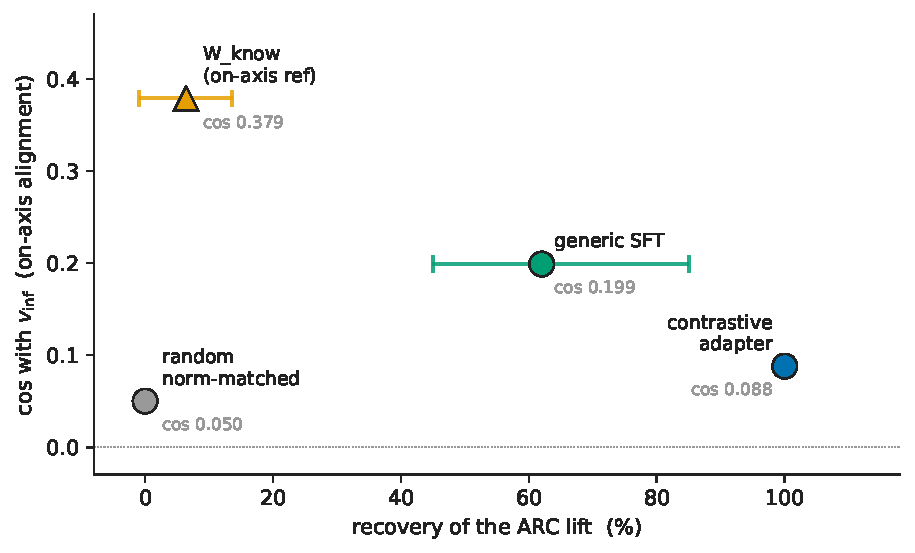
\includegraphics[width=\textwidth,alt={Scatter plot of the matched-control
spectrum: x-axis is the fraction of the ARC lift each direction recovers, y-axis is
the cosine with the functional correctness direction v_inf. Random floor near zero
recovery; the same-parameterization control near 37 percent at cosine 0.136;
higher-capacity generic SFT near 62 percent at cosine 0.199; the contrastive adapter
at 100 percent with the lowest cosine 0.094; and the on-axis reference W_know at high
cosine 0.379 but only 6.4 percent recovery.}]{figures/fig_geometry_spectrum.pdf}
\caption{\textbf{The matched-control spectrum on two independent axes.} $x$:
fraction of the ARC lift each direction recovers; $y$: cosine with the functional
correctness direction $\vinf$ (net effect on activations for the four methods; the
reference direction itself for $\Wknow$, marked $\blacktriangle$). The two orderings
are not monotone in each other: the most on-axis point ($\Wknow$, cos 0.379)
recovers only 6.4\%, while the top recoverer (the contrastive adapter, 100\%) is the
\emph{least} on-axis (cos 0.094). \textbf{The two non-contrastive controls separate
the two factors at work.} The \emph{same-parameterization} control (identical 48
head-pairs and $12{,}336$ parameters; only the objective differs) recovers
${\sim}37\%$ at cos $0.136$, while \emph{higher-capacity} generic SFT
($1{,}800\times$--$58{,}000\times$ more parameters) recovers ${\sim}62\%$ at cos
$0.199$: with the parameterization held fixed the contrastive objective is both
further off-axis and far more effective, whereas added capacity buys recovery while
moving \emph{toward} the axis. So how much a generic objective recovers depends on
capacity, and where the recovery lives depends on the objective --- two factors, not
one ordered scale. Horizontal bars are the published 95\% intervals on the recovery
fraction where one exists --- $\Wknow$ $[-0.9\%, +13.6\%]$ and generic SFT
$[51\%, 73\%]$ (paired bootstrap); the random floor (three seeds), the same-parameterization control
(three seeds, sd $5.0$ pp) and the contrastive anchor (100\% by construction) carry
none, and we do not synthesize one. \textbf{$\Wknow$'s interval crosses zero and
overlaps the random floor:} its 6.4\% is statistically indistinguishable from no
recovery (exact McNemar $p=0.136$), and it is counted with the floor rather than as a
rung. Values in \cref{tab:spectrum}.}
\label{fig:spectrum}
\end{figure}

\begin{table}[tbp]
\centering
\begin{threeparttable}
\caption{\textbf{Geometry spectrum: off-axis of degree, method-dependent.}
Apples-to-apples: the \emph{net effect on activations} of each method, decomposed
against the functional correctness direction $\vinf$. \code{ratio} = on-axis
alignment of the net effect with $\vinf$, normalized to a random direction (1.0 =
like random; higher = more on-axis than chance).}
\label{tab:spectrum}
\footnotesize
\begin{tabular}{L{3.2cm} L{6.2cm} L{2.8cm} L{2.6cm}}
\toprule
Direction & Recovery of the lift & cos with $\vinf$ (ratio vs chance) & Source
artifact \\
\midrule
random norm-matched (3 seeds) & $\mathbf{{\approx}0\%}$ (acc\_norm 0.50--0.52
${\approx}$ base 0.505) & 0.05 (1.0) & \code{msap-\allowbreak phase1-\allowbreak 20260624}
\code{derisk/\allowbreak offsets\_\allowbreak random\_\allowbreak s*} \\
on-axis maximum ($\Wknow$, Fisher-LDA) & $\mathbf{6.4\%}$ (ARC null 0.500 / mc
0.853 / wknow 0.522; \textbf{statistically indistinguishable from zero}: exact
McNemar b=10/c=19 $p=0.136$, paired-bootstrap frac-CI95 $[-0.009, +0.136]$ and
Wilson acc-CI $[0.474, 0.571]$ both include chance) & --- (cos with $\vinf$ 0.379;
cos with $\thetamc$ 0.0014) & \code{runs/\allowbreak wknow\_\allowbreak causal/\allowbreak } +
\code{msap-\allowbreak wknow-\allowbreak onaxis-\allowbreak 20260623} \\
contrastive adapter (net effect) & 100\% (by construction) & $\mathbf{0.088}$
\textbf{(1.74)}; across three seeds $0.094 \pm 0.008$ \textbf{($1.85 \pm 0.14$)};
direct $\thetamc$ offset cos 0.0014 & \code{msap-\allowbreak phase1-\allowbreak 20260624}
\code{derisk/\allowbreak contrastive\_\allowbreak direction}; \code{runs/\allowbreak v7\_\allowbreak lofit\_\allowbreak seed\{1,2\}/} \\
\textbf{same-parameterization control} (net effect, 3 seeds) --- \emph{same
intervention space, objective changed} & ${\sim}\mathbf{37\%}$ (ARC) &
$\mathbf{0.136 \pm 0.017}$ \textbf{($2.68 \pm 0.34$)} &
\code{runs/\allowbreak e1\_\allowbreak plain\_\allowbreak ce/\allowbreak neteffect\_\allowbreak seed*} \\
higher-capacity generic SFT (net effect) & ${\sim}\mathbf{62\%}$ & $\mathbf{0.199}$
\textbf{(3.93)} & \code{msap-\allowbreak phase1-\allowbreak 20260624} \code{derisk/\allowbreak align\_\allowbreak direction} \\
\bottomrule
\end{tabular}
\begin{tablenotes}[flushleft]\footnotesize
\item \textbf{Verdict.} All three methods are \textbf{mostly off-axis} (cos${<}0.2$,
${\sim}$78--85$^{\circ}$ from $\vinf$), but by different degrees, and the ordering is
informative: the contrastive adapter is the \emph{most} off-axis ($1.85$), the
same-parameterization control is intermediate ($2.68$), and higher-capacity generic
SFT is the least ($3.93$, $2.1\times$ more on-axis than the contrastive adapter)
$\rightarrow$ \textbf{off-axis of degree, not universal.}
\item \textbf{The same-parameterization arm is the load-bearing comparison here},
because it holds the intervention space exactly fixed (identical 48 head-pairs,
identical $12{,}336$ parameters) and changes \emph{only} the objective: with the
parameterization controlled, the contrastive objective lands
\textbf{further off-axis} ($1.85$ vs $2.68$) \emph{and} recovers substantially more
($100\%$ vs ${\sim}37\%$). The off-axis character is therefore not an artifact of the
LoFiT parameterization --- it tracks the objective.
\item \textbf{Two axes, not a ladder.} Recovery does not increase monotonically with
off-axis-ness: among the two \emph{non}-contrastive arms the more on-axis one
(higher-capacity SFT, $3.93$) recovers \emph{more} than the more off-axis one
(same-parameterization, $2.68$), because there capacity is the dominant variable. The
spectrum is organized by two factors --- objective and capacity --- and should not be
read as a single ordered scale.
\item The direct $\thetamc$ offset (cos 0.0014, a weight-space proxy) was misleading;
the clean net-activation-effect experiment is the canonical measurement.
\textbf{Forward filter:} a zero-cost read-space preview said ``off-axis'' (ratio
${\sim}1.05$); the clean experiment refuted it (3.93). Report only the clean
experiment.
\end{tablenotes}
\end{threeparttable}
\end{table}

% ------------------------------------------------------------------ Table 7 (6)
\begin{table}[tbp]
\centering
\begin{threeparttable}
\caption{\textbf{On-axis causal controls (no on-axis reference reproduces the
lift).} The earlier causal arms, consistent with \cref{tab:spectrum}'s spectrum:
pushing \emph{along} correctness does not recover the lift. (These on-axis causal
arms were measured on the vinf\_causal run, whose within-run MC baselines --- ARC
$+35.0$, TQA $+36.5$ --- differ slightly from the A1 canonical of
\cref{tab:headline}, $+37.25$; fractions are computed within-run.)}
\label{tab:onaxis}
\footnotesize
\begin{tabular}{L{5.4cm} L{6.6cm} L{2.8cm}}
\toprule
Quantity & Value & Source artifact \\
\midrule
ARC lift recovered by on-axis $\vinf$ (mass-mean, norm-matched) & fraction
$\mathbf{0.11}$ (MC $+35.0$ / VINF $+4.0$; $z = -6.63$, unpaired and conservative
--- the base stderr enters both lifts). \textbf{Paired over the same 400 items the
small recovery is detectable}: exact McNemar b=12/c=28 $p=0.017$, paired-bootstrap
frac-CI95 $[+0.027, +0.197]$ excludes 0. So the weaker on-axis reference recovers
\emph{little}, not \emph{nothing} --- unlike $\Wknow$ below &
\code{runs/\allowbreak vinf\_\allowbreak causal/\allowbreak vinf\_\allowbreak paired\_\allowbreak significance.\allowbreak json} +
\code{msap-\allowbreak vinf-\allowbreak causal-\allowbreak 20260623} \\
ARC lift recovered by $\Wknow$ (strongest on-axis ref) & fraction $\mathbf{0.064}$
(null 0.500 / mc 0.853 / wknow 0.522; ${\ll}$ 0.30 kill-rule;
\textbf{indistinguishable from zero}: exact McNemar b=10/c=19 $p=0.136$,
paired-bootstrap frac-CI95 $[-0.009, +0.136]$ includes 0) &
\code{runs/\allowbreak wknow\_\allowbreak causal/\allowbreak } \\
TQA lift recovered by either on-axis ref & $\mathbf{{\sim}0}$ (VINF $-2.75$;
$\Wknow$ ${\approx}$ null) & --- \\
$\thetamc$ vs $\vinf$ & $\coswh$ $\mathbf{-0.003}$ (within null); 6.4\% mass in top
PCs; norm $4.3\times$ class gap (the top-PC 6.4\% is coincidentally equal to the
$\Wknow$ recovery 6.4\%, not the same quantity) &
\code{theta\_\allowbreak mc\_\allowbreak character\allowbreak ization.\allowbreak json} \\
MMLU damage, on-axis $\vinf$ vs mc & VINF $-5.83$ ${\geq}$ MC $-4.30$ (gate PASS,
null MMLU $+0.07\pp$) & --- \\
\bottomrule
\end{tabular}
\begin{tablenotes}[flushleft]\footnotesize
\item \code{process-\allowbreak LoFiT-\allowbreak PRM} (an on-axis training program) is \textbf{refuted
causally} at eval time (a PRM corpus is not warranted); a \emph{training-time}
on-axis constraint \textbf{has now run and does not rescue transfer} (no $\lambda$
passes the lift-matched gate, so the $+35$ is the off-axis mass by
\emph{necessity}; see \cref{sec:open}).
\end{tablenotes}
\end{threeparttable}
\end{table}

% ------------------------------------------------------------------ Table 8 (7)
\begin{table}[tbp]
\centering
\begin{threeparttable}
\caption{\textbf{No layer locus: the lift scales with offset magnitude, not
layer.}}
\label{tab:locus}
\footnotesize
\begin{tabular}{L{5.6cm} L{6.6cm} L{2.6cm}}
\toprule
Quantity & Value & Source artifact \\
\midrule
corr(recovered lift, total offset magnitude $\Sigma|r|$) & $\mathbf{0.985}$ &
\code{msap-\allowbreak phase1-\allowbreak 20260624} \code{patch\_\allowbreak layers/\allowbreak *.\allowbreak json} \\
corr(recovered lift, head count) & 0.832 & same \\
``Layers 36--40 carry 87\%'' & head-count artifact (that band holds 71\% of adapter
heads); adapter spans L30--55 --- \textbf{not a causal locus} & same \\
\bottomrule
\end{tabular}
\end{threeparttable}
\end{table}

% ------------------------------------------------------------------ Table 9 (8)
\begin{table}[tbp]
\centering
\begin{threeparttable}
\caption{\textbf{Task heterogeneity: ARC ${\neq}$ TQA.} ARC is question-conditional
and carries the readout story; TQA is largely answer-prior / surface-form Goodhart.
The held-out + mc2 control has run: TQA generalizes held-out $\rightarrow$ reported
as a real, generalizing answer-prior lift, not as the off-axis mechanism.}
\label{tab:heterogeneity}
\footnotesize
\begin{tabular}{l L{3.6cm} L{6.2cm} L{2.8cm}}
\toprule
Task & Diagnostic & Value & Source artifact \\
\midrule
ARC & PMI-DC retention of lift & $\mathbf{78\%}$ (naive $+0.3275$ $\rightarrow$ PMI
$+0.2550$) & \code{pmi\_\allowbreak dc\_\allowbreak arc\_\allowbreak challenge.\allowbreak json} \\
ARC & choices-only lift & $\mathbf{+0.0375}$ CI$[-0.005, +0.08]$ (not clear) ---
question-conditional, not answer-prior &
\code{answer\_\allowbreak only\_\allowbreak arc\_\allowbreak challenge.\allowbreak json} \\
TQA & choices-only lift & $\mathbf{+0.2225}$ CI$[+0.1675, +0.2725]$ --- answer-prior
& \code{answer\_\allowbreak only\_\allowbreak truthfulqa\_\allowbreak mc1.\allowbreak json} \\
TQA & adapter picks correct option with NO question & $\mathbf{0.5725}$ (base 0.35,
chance 0.229) --- surface-form Goodhart
\citep{SurfaceFormCompetition,ChoicesOnlyCheater} & same \\
TQA & PMI-DC retention & 68\% & \code{pmi\_\allowbreak dc\_\allowbreak truthfulqa\_\allowbreak mc1.\allowbreak json} \\
TQA & paired significance of the $+37.25$ & exact McNemar b=6/c=155,
$p_{\mathrm{corr}}$ $\mathbf{6.26\times10^{-38}}$ (Holm $m{=}4$) & paired doc\_hash
400/400 \\
TQA & held-out generalization ${\neq}$ memorization (full set $n{=}817$; train
covers ${\sim}79.9\%$, 653 SEEN / 164 UNSEEN) & v7mc
$\mathbf{\Delta_{\mathrm{UNSEEN}}}$ \textbf{mc1} $\mathbf{+37.8}$ ${\approx}$
$\Delta_{\mathrm{SEEN}}$ $+36.9$; mc2 $\Delta_{\mathrm{UNSEEN}}$ $+26.1$ (gate
$\Delta_{\mathrm{UNSEEN}}$ mc1 ${\geq}+15$ AND $\Delta$mc2 ${>}+10$ passed); generic
Align \textbf{collapses held-out} (mc1 $+38.6{\rightarrow}\mathbf{+7.9}$; mc2
$+24.1{\rightarrow}+7.6$) & \code{analyze\_\allowbreak tqa\_\allowbreak contamination\_\allowbreak l4.\allowbreak py}, full 817 \\
\bottomrule
\end{tabular}
\begin{tablenotes}[flushleft]\footnotesize
\item \textbf{Note.} The lift is task-heterogeneous. TruthfulQA is an answer-prior
effect --- a generalizing selection lift on mc1/mc2 (the held-out + mc2 control
generalizes: $\Delta_{\mathrm{UNSEEN}}$ mc1 $+37.8$, so it is neither memorization
nor mc1-only, while a generic Align control collapses held-out to $+7.9$) --- but
it is not a truthfulness gain and not evidence for the off-axis mechanism. ARC is
question-conditional, off-axis-of-degree, and non-transferable.
\end{tablenotes}
\end{threeparttable}
\end{table}

% ------------------------------------------------------------------ Table 10 (9)
\begin{table}[tbp]
\centering
\begin{threeparttable}
\caption{\textbf{Deployment pathologies (coupled to injection method, not to the
lift).} The recovery introduces \textbf{two certified costs} --- no transfer to
generative CoT (multi-step reasoning breakage) and retrieval/recall spillover ---
that a generic SFT recovering most of the lift does not incur, so they trace to how
the contrastive offset is folded into weights, not to the lift itself. A third,
previously-listed cost --- an end-of-turn ``collapse'' --- is \textbf{retracted} as
a measurement artifact (last row). Rows 2--4 are \textbf{family} evidence from
sibling adapters (the D.1 SocialIQA and B.2/KR adapters), not the V7-mc adapter
under study; V7-mc's own directly-measured MMLU spillover is $\mathbf{-4.2\pp}$
(row 5).}
\label{tab:pathologies}
\footnotesize
\begin{tabular}{L{3.4cm} L{9.0cm} L{2.4cm}}
\toprule
Pathology & Value & Source artifact \\
\midrule
No-CoT-transfer (multi-step reasoning) & gsm8k loss every condition
(\cref{tab:genface}); contrastive baked ${\rightarrow}0.17$. \textbf{R6 canonical
(kill-rule PASS, apples-to-apples, template ON, 5-shot, $n{=}400$):} base
$\mathbf{0.9775}$ vs v7mc $\mathbf{0.7275}$ = $\mathbf{-25\pp}$, flat across cap
\{512, 2048\}=0.7275/0.7275 $\rightarrow$ \textbf{not truncation} (extra budget
never rescues; v7mc cap2048 runs ${\sim}$2h to the ceiling without improving;
template-OFF is worse --- base 0.730 / v7mc 0.035, $-69\pp$ --- so it is not a
template artifact). Forensic (R6probe @cap2048): 79 clean-wrong (\code{\#\#\#\#}
wrong number --- reasoning resolved but defective) + 26 degenerate non-terminating
loops already present @cap512 (the loop precedes the budget, not truncation).
\textbf{Align SFT preserves $0.96{\rightarrow}0.95$ (NS)} & R6
(\code{runs/\allowbreak mechanism\_\allowbreak v8/\allowbreak R6\_\allowbreak *}) + R6probe (\code{R6probe\_\allowbreak *}) +
\cref{tab:genface} \\
\addlinespace
Retrieval spillover (D.1 SocialIQA adapter --- family evidence) & MMLU
$\mathbf{-19.59\pp}$ ($0.8306{\rightarrow}0.6347$); K=12 not recovered ($-20.80$,
Pareto-worse) & D.1 SocialIQA spillover audit \\
Spillover (KR SciQ K=24) & GPQA Diamond $\mathbf{-12.1\pp}$ (sciq $+2.1\pp$
overshoot) & KR SciQ K=24 overshoot audit \\
Spillover (B.2 mc\_discrimination) & MMLU $-6.3\pp$ / GPQA $-6.6\pp$ & B.2 phase-3
findings \\
Spillover MMLU (V7-mc direct, eval-bulletproof R10) & $\mathbf{-4.2\pp}$
($0.8226{\rightarrow}0.7805$, ${\sim}$2k stratified, 0-shot) --- the V7-mc adapter
under study spillovers MMLU itself; same sign as B.2 ($-6.3\pp$), smaller &
\code{runs/\allowbreak eval\_\allowbreak bulletproof/\allowbreak R10\_\allowbreak *} \\
Spillover mechanism & $\coswh(\vinf, \vret)$ $\mathbf{+0.283}$
BCa95$[+0.276, +0.291]$, null ${\pm}0.007$, $n{=}316$ --- orthogonality refuted;
co-location on a shared substrate & functional-axis geometry analysis \\
\addlinespace
\sout{End-of-turn collapse} \textbf{retracted --- eos-token artifact} (was: D.1
social $56{\rightarrow}4$, D.1 factual $48{\rightarrow}4$, V7-mc factual
$48{\rightarrow}4$/$60{\rightarrow}4$) & \code{eval\_\allowbreak adaptive\_\allowbreak verbosity} scored
termination on \code{tokenizer.\allowbreak eos\_\allowbreak token\_\allowbreak id} (\code{<eos>}) but Gemma~4 closes a
turn with \code{<end\_\allowbreak of\_\allowbreak turn>} (106). Corrected re-measure
(\code{\_\allowbreak resolve\_\allowbreak stop\_\allowbreak ids}): base\_factual $48{\rightarrow}\mathbf{100\%}$,
v7mc\_factual $4{\rightarrow}\mathbf{100\%}$ --- \textbf{no collapse}; v7mc factual
answers are correct + terse + terminate (``Paris''/``Au''/``1945''); the
``degenerate loop'' read earlier was junk \emph{after} \code{<end\_\allowbreak of\_\allowbreak turn>}. The
analogous D.1 cells were re-measured: no ${\rightarrow}4\%$ collapse, only a modest
open-ended-generation degradation (social $96{\rightarrow}76\%$, creative
$68{\rightarrow}12\%$), adapter-dependent and off the V7-mc headline. & buggy:
\code{EOS\_\allowbreak v7mc\_\allowbreak smoke.\allowbreak json}; fix:
\code{mechanism\_\allowbreak v8/\allowbreak EOS\_\allowbreak verbosity\_\allowbreak fixed.\allowbreak json} \\
\bottomrule
\end{tabular}
\end{threeparttable}
\end{table}

\subsection{The causal spine replicates in a second model
family}\label{results:qwen}

Everything above is one model. We repeated the causal decomposition on
Qwen2.5-14B-Instruct --- a different family, different tokenizer, different
pre-training --- with the same pipeline and $6{,}192$ trainable parameters, in two
runs. A gated reference run established the \emph{effect} on this family: a same-sign
cold-MC lift on all four tasks (ARC $+18.0$ / HellaSwag $+7.8$ / TruthfulQA-mc1
$+15.8$ / Winogrande $+3.0$), with the null-adapter arm exactly at base
(\cref{disc:status}). The decomposition run reproduces it at
$+16.25 / +7.25 / +15.00 / +3.25$, inside the ${\pm}3$ pp band fixed before looking:
ARC acc\_norm moves $0.4975 \rightarrow 0.6600$, a lift of $\mathbf{+16.25}$ pp,
smaller than Gemma's $+35.83$ but built by the same machinery. That run's
null-adapter arm sits $1.5$ pp above the reference and its adapter arm $-0.25$ pp ---
mixed signs, the signature of BF16 non-determinism rather than the one-directional
${\approx}24$ pp a broken chat template produces --- so every fraction below divides
by \emph{this} run's own base and adapter, never across runs.

The decomposition transfers with it. Splitting the trained offset against the
functional inference direction and re-injecting each part separately, the
\emph{off-axis} component carries the lift ($\text{off\_perp} = \mathbf{+106.2\%}$
recovery) while the on-axis component does not ($\text{off\_par} = -6.2\%$), and the
strongest on-axis direction we can build recovers $-18.5\%$ --- as in Gemma, the
on-axis arm buys nothing. The learned direction is privileged rather than merely
orthogonal: three norm-matched random directions inside the same complement recover
$-16.9 / -16.9 / -13.8\%$ (mean $-15.9 \pm 1.8$), so $\text{off\_perp}$ clears its own
noise floor by ${\sim}122$ pp in the same units, against ${\sim}101$ pp in Gemma.
Read against that floor, the on-axis arm does not beat same-norm noise in
\emph{either} family.

Non-transfer to generation replicates too, and harder: gsm8k falls
$0.945 \rightarrow 0.455$, $\mathbf{-49.0}$ pp, twice Gemma's $-24.2$. Crucially the
turn-termination rate is preserved ($1.000 \rightarrow 0.985$), with stop ids
resolved from the model's own generation config --- so the damage is multi-step
reasoning, not the EOS collapse an earlier counting bug once suggested
(\cref{tab:pathologies}). Generation also shortens, $191 \rightarrow 133$ tokens on
average.

Two honest limits on how far to read this. First, \textbf{this is replication in two
families, not universality}: two points do not establish a law, and the arms differ in
magnitude throughout. Second, two cells are not readable here and we do not report
them as agreement: Winogrande's lift is only $3.25$ pp, too small a denominator for a
recovery fraction to mean anything, and the shuffle floor on HellaSwag comes out
\emph{positive} ($+31\%$) rather than near zero. The matched non-contrastive control orders the tasks
HellaSwag $114.9\% >$ ARC $27.2\% >$ TruthfulQA $-58.3\%$, the same ordering Gemma
gives \emph{under acc\_norm} --- a caveat that matters, because under raw accuracy the
ordering does not survive in either family (\cref{lim:metric}).

\subsection{The lift is not an artifact of saturated benchmarks: MMLU-Pro}
\label{results:mmlupro}

Every anchor above sits near the base's chain-of-thought ceiling, which invites the
obvious objection: perhaps the exploit only exists on easy four-option benchmarks the
model has effectively already solved. We tested it on MMLU-Pro --- ten options,
chance $0.100$, and a base that scores $\mathbf{0.2610}$ cold, barely $2.6\times$
chance. It is not saturated by any reading. Four arms, $1{,}000$ items, paired on
every \code{doc\_id}.

\textbf{The lift appears anyway.} The adapter scores $0.3830$ against the base's
$0.2610$: $\mathbf{+12.20\pp}$, CI $[+9.10, +15.30]$, with disjoint Manski bounds
(the cold channel has no unparsed items, so the bounds are the point estimates).
Because the metric ordering burned us once before (\cref{lim:metric}), we recomputed
under both defensible definitions: raw argmax reproduces the scored prediction
$1{,}000/1{,}000$ in every arm, and the lift is $+12.20$ under plain acc and
$\mathbf{+15.00}$ CI $[+11.70, +18.20]$ under acc\_norm. The two
non-contrastive arms separate as the inducibility spectrum predicts: the
higher-capacity LoRA moves $+5.10$ CI $[+2.50, +7.80]$, while the
\emph{same-parameterization} plain-CE arm --- the one that recovers $36.2\%$ on ARC
--- is null under both definitions here ($-0.60$ CI $[-3.10, +2.00]$ and $+0.50$ CI
$[-2.10, +3.10]$), the same collapse it shows on TruthfulQA-mc1 and further evidence
that inducibility is task-dependent rather than a constant of the objective.

\textbf{And it still does not transfer.} Under chain-of-thought the paired difference
is $-8.00\pp$, CI $[-10.90, -5.10]$: the interval excludes zero on the wrong side of
zero, which is not transfer. We do not declare even that much --- the three-way
Manski bounds \emph{overlap} ($[0.604, 0.845]$ against the base's
$[0.684, 0.905]$), so the honest statement is that the scoring lift buys nothing
generative here, not that it costs something.\footnote{These bounds were recomputed
after we found that the harness's \code{unparsed} field does not count truncated
traces; the real denominator was ${\sim}5\times$ larger (base 41 against 221). The
conclusion did not change and now holds a fortiori, since widening the unknown set
can only widen both brackets.}

What this widens, and what it bounds, are different things. It widens the
\emph{scope}: the phenomenon is not a property of saturated four-option benchmarks.
It bounds the \emph{magnitude}: $+12.20$ here against $+35.83$ on ARC is roughly a
third. Task-to-task variation of that size is already on record for this objective,
albeit as a different quantity --- the fraction of the lift a generic control
recovers, which runs Winogrande $79.5\%$ / HellaSwag $69.5\%$ / ARC $36.2\%$ /
TruthfulQA $0.9\%$ (\cref{results:generic}).

The result also sharpens what the GPQA null in \cref{results:arbiter} does and does
not show. Both benchmarks are hard and unsaturated, and both leave the base
substantial cold-to-CoT headroom --- GPQA ${\sim}23\pp$ ($0.4747 \rightarrow
0.7071$), MMLU-Pro ${\sim}44\pp$ ($0.2610 \rightarrow 0.7060$) --- yet the adapter
recovers approximately nothing on the first and $+12.20\pp$ on the second. Difficulty
therefore does not govern whether the exploit fires. What the two benchmarks
\emph{do} differ in is whether the adapter's training distribution covers them, and
only the covered one lifts --- a protocol-bound inference, since we vary benchmark
identity rather than manipulating distance directly, and benchmark identity carries
format, domain and option count with it. That is the same conclusion \cref{disc:arbiter}
reaches with its within-format controls, arrived at here by varying the benchmark
instead of the format, and it is what ``an in-distribution exploit of a lossy
readout'' predicts.

Finally, the generative pathology reproduces in its now-familiar form: degeneration
rather than degraded reasoning. Repetition loops (distinct-4 $< 0.35$) run
\textbf{0/1{,}000} for the base against $146$ for the adapter and $298$ for plain CE ---
an ordering that replicates on a second benchmark (\cref{disc:pathologies}).

Two caveats bind this section. None of the four arms is replicated. And it is not the converse arm
we flag in the limitations (\cref{lim:anchors}): the adapter here was trained on the same corpus as everywhere
else and \emph{evaluated} on MMLU-Pro, so it answers whether the effect survives an
unsaturated benchmark, not whether contrastive PEFT trained in-distribution on one
would produce it.

\section{Discussion: the mechanism of the recovery}\label{sec:discussion}

The scoring-face gain documented above invites a natural reading: the
contrastive-correctness adapter sharpens the model's internal direction for answer
correctness, so that cold multiple-choice scoring becomes more accurate. This
section shows the gain is better understood as a \emph{quantified causal
attribution} than as a sharpening. We take as established setup that cold
multiple-choice scoring under a chat template under-expresses knowledge the model
holds (\cref{sec:related}; \citealp{ConfidenceManifold,InsideOut,KAPPA}); the
result is what the adapter does about it. Most of the recovery is what
\emph{generic} fine-tuning buys (\cref{disc:inducibility}); it lives in a learned
direction that is off-axis-of-degree to the model's correctness geometry and is
causally privileged within that off-axis complement (\cref{disc:geometry}); it has
no layer locus (\cref{disc:locus}); and it does not transfer to generation
(\cref{disc:pathologies}).

The off-axis geometry is not a curiosity but the \emph{expected} signature of the
attribution we lead with, and reading it that way organizes the rest of this
section. The cold readout does not fail for lack of knowledge; it fails by
\textbf{surface-form swamping}: on the items the adapter fixes the base buries the
gold beneath more fluent distractors (\cref{disc:arbiter}). Plausibly, though we do
not measure this, suppressing surface form need not align with signalling
correctness. The two causal arms make the point in opposite directions: injecting
correctness \emph{on-axis} (the strongest on-axis reference we can build, $\Wknow$)
recovers only $\mathbf{6.4\%}$ of the lift, which refutes a knowledge-deficit
account; pushing \emph{off-axis} (perpendicular to correctness, $\offperp$) recovers
${\sim}$\textbf{100\%}, which is consistent with the surface-swamping account. The
off-axis direction is therefore not a spurious accident but a natural form for a
fix to take when the pathology is one of format rather than of knowledge --- which
is why a single off-axis push unifies the readout result (\cref{disc:arbiter}), the
inducibility attribution (\cref{disc:inducibility}), the on-axis null
(\cref{disc:geometry}), and the deployment pathologies (\cref{disc:pathologies}).

\subsection{The fixed items are chain-of-thought-accessible, the no-transfer is
out-of-task (not difficulty-bound), and the readout misranks by confident burial}
\label{disc:arbiter}

The cleanest evidence that the readout --- not the model's knowledge --- is the
bottleneck comes from a per-item arbiter. We isolate the \textbf{124} ARC items the
adapter corrects in cold multiple-choice scoring but the on-axis offset does not
(\cref{disc:geometry}), and for each ask whether the \emph{base} model already
reaches the right answer through generative chain-of-thought. It does: the base
solves $\mathbf{124/124}$ ($1.000$) of these items under generative CoT (the
fixed-parser re-run resolves the earlier 123/124: the one ``failure'' was a parser
artifact --- doc 128's numeric option label ``4'', which the letter-parser could not
emit by construction --- now parsing correct, n\_unparsed $5{\rightarrow}0$),
indistinguishable from its CoT accuracy on the items it already scores correctly
cold (base-right control, $200/202 = 0.990$ --- read from the same fixed-parser run,
not from the superseded pre-fix one, where it was 196/202). The items the adapter
``fixes'' are knowledge the base already reaches by reasoning; cold scoring simply
misranks them.

\paragraph{The arbiter discriminates: a negative control on the adapter's
residual.}
A per-item arbiter of this shape invites an obvious objection --- if the base
solved \emph{everything} under chain-of-thought, ``the fixed items were already
CoT-accessible'' would be true of all of ARC and would say nothing about the
adapter. The control is the complementary population, and it needs no new
generation: the v2 arbiter run already covers all 400 items under the identical
protocol (greedy $k{=}1$, same prompt, same fixed parser, \code{n\_\allowbreak unparsed=0}), so
re-partitioning it is protocol-identical to the headline by construction. On the
adapter's \textbf{residual} --- the 47 base-wrong items it does not fix --- the base
solves $\mathbf{41/47 = 0.872}$ (CI $[0.748, 0.940]$), against $\mathbf{151/151}$ on
the base-wrong items it does fix (Fisher $p=1.4\times10^{-4}$) and
$\mathbf{392/400 = 0.980}$ over all of ARC ($p=0.0015$). A related partition in the
independent premise-file scaffold --- which defines the $n{=}73$ residual of the PMI
residual-discrimination analysis below; the calibration analysis runs on the lm-eval
scaffold --- agrees: $66/73 = 0.904$ against $326/327 = 0.997$,
$p=3.6\times10^{-5}$. It is \emph{related} rather than identical, and we say so: the
lm-eval partition conditions on base-wrong (47 against 151), while the $n{=}73$ is
every item the adapter gets wrong, including 8 it broke from base-right. Restricting
it to base-wrong for a like-for-like read gives $58/65 = 0.892$, between the two. So
the 124/124 is not trivially true of all of ARC. Two honest qualifications travel
with it. First, the magnitude is modest in absolute terms --- ARC is near its CoT
ceiling everywhere, and the discrimination is 0.872 against 0.980, not against
something far lower. Second, the residual figure fell \emph{between} the two
thresholds we pre-registered for this control (${\leq}0.85$ $\rightarrow$
discriminates, ${\approx}0.97$ $\rightarrow$ saturated); we therefore rest the
reading on the contrast and its interval (CI upper 0.940 excludes the saturated
value) rather than on the point estimate clearing a bar it did not clear. The
adapter is a \emph{shortcut} to that knowledge --- it nudges the scoring logits
toward answers the base could reason its way to, without reasoning.

This directly explains why the lift does not transfer to generation
(\cref{sec:results}): on exactly these items the base is already at ceiling under
CoT, so there is no generative headroom for a scoring shortcut to add. The obvious
objection is that ARC is simply easy --- near its CoT ceiling --- so the arbiter
cannot tell ``recovers knowable'' from ``fabricates plausible.'' We corroborate the
no-transfer out-of-task.

On \textbf{GPQA}, where the base must genuinely reason, its CoT accuracy is
$\mathbf{0.7071}$ (arbiter; 140/198, thinking-on, with the generation budget raised
to 8192 tokens --- at 2048 the base truncated 96\% of its reasoning, producing a
spurious 0.15). Two things follow. First, 0.7071 is well above chance, so the base
\emph{does} solve these by reasoning; yet the cold-scoring shortcut still has no
generative headroom to add, and indeed the measured cold-MC lift on GPQA is
${\sim}0$ (base $0.4747 \rightarrow$ adapter $0.4697$, $-0.5\pp$, CI crossing zero)
--- the no-transfer result restated out-of-task. This is a
no-transfer-\emph{out-of-task} result, not a no-transfer-to-\emph{hard} one: GPQA is
out-of-task and distribution-distant (it is the B.2 spillover task at $-6.6\pp$).
Second, because the base already reasons GPQA out, a verifier-guided arm (base
generates, adapter scores) has nothing to harvest, so we did not build one (a design
choice following from the result, not an independent test). The
readout-is-the-bottleneck result therefore survives an out-of-task control that the
ARC arbiter alone could not provide.

Two added controls now separate difficulty from distribution, where previously a
single out-of-task benchmark could not. \emph{Within-format difficulty:} the cold-MC
fix-rate on base-wrong items moves only $\mathbf{-0.10}$ as ARC difficulty rises
(ARC-Easy 0.861, $n{=}360$ $\rightarrow$ ARC-Challenge 0.763, $n{=}198$, both
burial-matched by gold-rank), whereas it collapses $\mathbf{-0.56}$ going
out-of-task to GPQA (0.202) --- so \emph{distribution}, not within-format
difficulty, drives the collapse. \emph{A second pair of anchors:} on HellaSwag and
Winogrande, where the lift also holds ($+17$ / $+19$), the base's CoT accuracy is
high (0.83 / 0.9425) --- like ARC's 0.97 and well above GPQA's 0.70 --- and the
recovery is recoverability-gated (the adapter fixes CoT-right items more than
CoT-wrong ones: HellaSwag 0.64 vs 0.31, Winogrande 0.76 vs 0.42), i.e.\ the lift
rescues knowledge the base can already reason out. The no-transfer is therefore
\textbf{out-of-task, not difficulty-bound} --- supported now, not merely
suggestive, on all three anchors. \emph{(Power caveat: the hard cells are small ---
HellaSwag $n{=}32$, Winogrande $n{=}12$ --- and the Easy${\rightarrow}$Challenge
difficulty range stays below GPQA's, both base-CoT near 0.97; the burial gradient is
shallow throughout, corr(fix, z-gap) $-0.17$.)}

\paragraph{How the readout misranks on ARC: confident burial under fluency.}
The arbiter shows the model \emph{has} the answer; a calibration analysis on ARC
shows \emph{how} cold scoring loses it, and it is not indifference between close
options but misplaced confidence. We measure this on an \textbf{adapter-independent}
subset --- the $n{=}192$ ARC items the base scores wrong cold yet solves under CoT
($S_{\mathrm{cot\_coldwrong}}$, defined without any reference to the adapter) --- so
the signature cannot be an artifact of which items the adapter happened to fix. On
these items the base's chosen (wrong) option beats the gold by $\mathbf{1.45\sigma}$
within-item, the gold sits at \textbf{median rank 2 of 4} (only 41\% have the gold
at rank 1), and a gold-vs-distractor ranking on the base-wrong items scores
\textbf{AUC 0.394, \emph{below} chance}. (This confident-wrong signature is the
multiple-choice overconfidence aligned-model calibration work documents, which
separates an \emph{answer-decision} uncertainty from a \emph{format-preference}
uncertainty and attributes alignment overconfidence to their conflation
\citep{AlignedMCCalibration}; our claim goes past calibration --- the per-item
arbiter shows the buried answer is \emph{reachable}, at 124/124 under CoT, and a
learned offset \emph{exploits} the gap rather than re-calibrating it post hoc.) The
gold is not a flat near-miss; it is actively \emph{buried} beneath more fluent
surface forms --- the base's raw pick is the gold only \textbf{19\%} of the time
here, against \textbf{81\%} on the items it scores correctly cold.

The re-ranking the adapter performs is \textbf{promotion-dominated} (it adds 0.35 of
probability mass to the gold while removing 0.21 from wrong options, and sharpens
the distribution, $\Delta$entropy $-0.19$), consistent with surfacing a
buried-but-present signal rather than manufacturing one.

\emph{Methodological note we are forced to make:} the apparent \emph{flatness} of
the char-normalized answer entropy (0.920 on this subset) is a softmax-temperature
artifact --- length normalization compresses the spread ${\sim}50\times$ without
reordering, while the raw distribution is peaked. We therefore report \textbf{rank
and within-item z-gap}, which are invariant to that normalization, and not entropy,
whose flatness flips with the metric. (The selection-conditioned
$S_{\mathrm{flip}}$ subset, the 151 items the adapter flips, shows the identical
signature --- z-gap $1.37\sigma$, gold-rank median 2 --- and serves only as a
consistency check; its conditioning on the adapter's flips is why the
adapter-independent subset is the headline.)

This burial-and-recoverability signature is established on ARC; we \textbf{could not
detect} it out-of-task on GPQA, but as a power-starved non-finding rather than a
contrast: on the burial-matched hard cell the CoT-right and CoT-wrong fix-rates are
equal ($0.186 = 0.186$), but $n{=}43$ with 31 items left unparsed ($k{=}1$ greedy
decoding) contaminates that cell, leaving it indistinguishable from no measurement.
We therefore report the recoverability-gating as \textbf{could-not-detect /
power-starved out-of-task}, not as evidence against it.

\paragraph{The signal is swamped, not absent --- ``broken'' means \emph{lossy}.}
It does not follow that the cold channel is empty. After removing length and fluency
(a PMI / decision-conditional residual), a gold-vs-distractor discrimination scores
above chance on both arms in the \emph{same scalar channel}: \textbf{AUC 0.574} (CI
$[0.520, 0.627]$) on the base-wrong items ($n{=}204$), and \textbf{0.667} (CI
$[0.584, 0.744]$) on the adapter's own residual ($n{=}73$, the items it does not
fix). The correctness signal is present in the cold channel but \emph{out-ranked} by
fluency, not erased: the same PMI-residual channel carries gold-vs-distractor
signal, rather than the channel being empty and the adapter supplying missing
knowledge.

\emph{Honesty boundary:} these are two arm readings on \textbf{different
populations} ($n{=}204$ vs $n{=}73$), not a within-set rise; and the base-arm CI
lower bound, 0.520, does not on its own clear a 0.55 ``present'' threshold --- we
call the base channel \emph{intermediate} and rest the present-but-swamped claim on
the adapter arm (CI lower bound $0.584 > 0.55$), and raising power on the base arm
did not rescue it: pooling base-wrong with $S_{\mathrm{cot\_coldwrong}}$ --- and
every defensible pool variant --- ran, and none clears 0.55. The
adapter-independent $S_{\mathrm{cot\_coldwrong}}$ ($n{=}192$, the items the base
\emph{provably} knows via CoT yet cold-MC misranks) reaches only CI lower bound
0.512, and even the literal union base-wrong ${\cup}$ $S_{\mathrm{cot\_coldwrong}}$
($n{=}228$, which is \emph{pro}-gate --- its 24 extra items are base-right under
premise scoring) reaches 0.535, so the base channel stays \emph{intermediate} on the
strongest honest pool.

\subsection{Much of the recovery is generic to fine-tuning; how much depends on
capacity and on the task}\label{disc:inducibility}

If the lift were a specific consequence of the \emph{contrastive-correctness}
objective, an ordinary supervised fine-tune should not reproduce it. It largely does
--- and running the control at two very different capacities shows that ``how much''
is not a single number.

\textbf{At the adapter's own capacity.} The same-parameterization control
(\cref{method:neteffect}: identical 48 head-pairs, identical $12{,}336$ trainable
parameters, identical corpus/steps/split/checkpoint rule, ordinary cross-entropy on
the correct answer only, three seeds) recovers $\mathbf{36.2\% \pm 5.0}$ of the ARC
lift, or $39.7\% \pm 3.1$ if the fixed final step is used instead of the
best-validation checkpoint --- a ${\sim}36$--$40\%$ range. Because the intervention
space is held exactly fixed here, this is the arm that attributes recovery to the
objective as such.

\textbf{At $1{,}800\times$--$58{,}000\times$ capacity.} A non-contrastive Align-LoRA
on the same data budget, run through the same causal recovery machinery (a sign-safe
three-zone control gate), recovers about \textbf{62\%} of the ARC lift, and that
fraction is \textbf{flat across a rank sweep} (r8/32/64/256: 59/63/60/65), with the
sweep slope's confidence interval spanning zero ($[-1.4, +3.4]$) and a
paired-bootstrap fraction interval of $\mathbf{[51\%, 73\%]}$. That interval resamples
the $400$ items with replacement and carries the base, generic and contrastive arms
together, so the positive inter-arm correlation the three arms actually have
(item-level $r{=}0.42$ between base and generic) is retained instead of discarded; it
is $44\%$ narrower than, and contained in, the delta-method $[45\%, 85\%]$ we report
as the conservative reading (zone C is binned on the point estimate, $0.62$, and is
unchanged). One-sided, the fraction exceeds one half in $98.2\%$ of resamples --- one
minus the one-sided bootstrap $p$-value, not a posterior probability. Under raw
accuracy instead of length-normalised accuracy the point moves to $0.61$ and that
figure to $96.9\%$. Within that grid, then, the
residual is not a gap more rank closes; but the comparison with the
same-parameterization arm shows that capacity itself moves the fraction, from
${\sim}37\%$ to ${\sim}62\%$. We therefore do not name a ceiling for generic
fine-tuning, and we treat the contrastive-specific residual as \emph{grid-relative}:
${\sim}60$--$64\%$ of the ARC lift at equal capacity, ${\sim}38\%$ against the
higher-capacity arm.

One caveat we apply to ourselves, symmetric with the information-set discipline of
\cref{disc:channel}: matching examples and optimizer steps does not match the
effective training signal per step --- the contrastive objective sees each example
with an explicit correct/incorrect contrast where the plain objective sees only the
correct completion --- so these fractions attribute the lift to \emph{fine-tuning on
this data} rather than to any stronger claim of per-step informational equivalence.
Indeed the task breakdown suggests that contrast is exactly what the harder cases
need: the same three same-parameterization seeds recover $79.5\% \pm 1.4$ of the
Winogrande lift and $69.5\% \pm 6.4$ of HellaSwag's --- where scoring rewards the
plausibility of a continuation --- but $0.9\% \pm 3.3$ of TruthfulQA-mc1's, where a
plausible distractor must be beaten, despite TruthfulQA sitting in the control's own
training corpus. ARC, at ${\sim}37\%$, falls between the two regimes.

We restrict this control to ARC because TruthfulQA's matched corpus leaks into its
evaluation. Across the rank sweep the TQA recovered fraction rises monotonically
(41/66/72/91), the signature of memorizing training examples that recur at test;
held out on 20\% of TQA, the highest-rank control collapses from 98\% to 30\%
recovery and the rank sweep flattens (r8 = r256 = 0.524), while the contrastive
adapter still generalizes held-out (0.83). The matched corpus (TQA train-80\%, seed
0) overlaps the evaluation set; TQA is therefore excluded from the inducibility
control, and the ${\sim}62\%$ generic figure is an ARC result.

\subsection{The lift does not reduce to an interpretable re-scoring of the output
scalars}\label{disc:channel}

The inducibility result attributes most of the lift to generic fine-tuning, but it
leaves a sharper question: whether the recovered signal is a simple, interpretable
re-weighting of the scores the cold readout already produces (length, PMI, an
answer prior, a calibration temperature). If so, the ``lost'' knowledge would be
recoverable by post-hoc re-scoring alone, without touching the model's activations.
It is not. We build the strongest such re-scorer we can --- a supervised, held-out,
AUC-objective combination of the interpretable surface features (conditional
log-likelihood, answer-only log-likelihood, character length, PMI) --- and ask how
well it separates gold from distractor on the base-wrong items. It caps at
\textbf{AUC 0.574} (a held-out logistic fit at 0.458 and a non-linear GBM at 0.462,
an on-test-tuned oracle stack at 0.502, PMI alone at 0.574), against the
\textbf{adapter's 0.830} on the same items. PMI does not merely fail to match the
adapter --- applied \emph{to} the adapter it \emph{hurts} it
($0.818 \rightarrow 0.758$), and the adapter's re-ranking is only \textbf{2.4\%}
explained by the surface features ($R^2$ 0.024). The recovered signal therefore
lives \textbf{upstream of the collapsed output scalars}: no re-scoring of those
scalars recovers the lift, which answers the ``your baseline is just under-fit''
objection --- the ceiling is supervised and held-out, not a hand-tuned stack.

We are deliberate about what this licenses. The comparison is
\emph{information-set-confounded} --- the adapter mutates \textbf{activations},
whereas the surface stack re-weights \textbf{collapsed output scalars} --- so the
gap (0.830 vs 0.574) does \textbf{not} license ``a magic off-axis direction'' (a
generic SFT recovers ${\sim}62\%$ the same way, \cref{disc:inducibility}) nor ``an
empty channel'' (the residual is $0.574 >$ chance, \cref{disc:arbiter}). The
defensible claim is about the \textbf{channel}: the lossy readout discards signal
that survives in the activations and is not reconstructible from its own outputs.

We can now sharpen the channel claim with a same-space probe. A logistic probe fit
on the \emph{same} per-head \code{o\_\allowbreak proj}-input activations the adapter writes to
--- no fine-tuning, held out by item, on the same cold-MC option-continuation
distribution, scaler${\rightarrow}$PCA${\rightarrow}$logistic with the preprocessing
fit inside each fold and a within-item label-permutation null --- recovers
gold-vs-distractor on ARC base-wrong items at \textbf{AUC 0.955} (CI
$[0.934, 0.973]$, permutation null 0.494), far above the \textbf{0.502}
collapsed-output ceiling. A surface-form control --- the same probe on length/format
features of the option string --- caps at \textbf{0.442} (${\approx}$ chance), so
the 0.955 reads correctness the output scalars discard, not a length/format
artifact. This \textbf{widens and cleans the channel gap}
($0.502{\rightarrow}0.955$) relative to the scalar-stack version
($0.574{\rightarrow}0.830$).

We are careful about what it does \textbf{not} license. First, the probe reads
12288 activation dimensions while the adapter is constrained to nudge output logits.
The two are not on the same axis, so 0.955 is \textbf{not} ``the probe beats the
adapter,'' and we do not read it as a representational \emph{edit}. Second, that a
linear probe decodes correctness from activations at ${\sim}0.95$ is a
near-universal property of capable language models
\citep{AzariaMitchell,MarksTegmark}. It shows the information \emph{exists} in the
activations the readout collapses, \textbf{not} that the model's own deployed
readout is ``merely miscalibrated.'' We therefore make a \textbf{sharpened channel
claim} --- the cold-MC output-scalar channel is lossy relative to the activation
channel --- and we do \textbf{not} assert ``pure miscalibration'' or ``signal intact
upstream'' as anything beyond that channel statement.

Third, the recoverable signal is \textbf{broadly distributed}: a random 48-head set
decodes it as well (0.949 ${\approx}$ the adapter's 48 heads), so the probe speaks
to the cold-MC channel being lossy \emph{model-wide}, not to the adapter's subspace
being privileged. This is a read-test about the channel, decoupled from the
write-tests that establish the adapter's specificity (a random norm-matched
\emph{offset} recovers ${\sim}0\%$ of the \emph{lift}, \cref{disc:geometry}, a
different operation). On TruthfulQA the same probe reaches 0.974, but its
surface-form control is non-trivial (0.639, with a gold-first position artifact at
1.000), consistent with TruthfulQA's answer-prior character
(\cref{disc:heterogeneity}); the channel claim is therefore anchored on ARC.

\subsection{A read-only selector deploys the recovered signal without the
pathologies}\label{disc:selector}

The channel result has a constructive consequence --- but we scope it as the
\emph{read leg of a read${\neq}$write dissociation}, not as a new method, because
the bare capability is already published. That a read-only probe or readout can
\emph{select} multiple-choice answers and recover an accuracy lift, with no weight
edit and no generation, is established by at least two independent mechanisms: NoVo
selects answers by voting over truth-correlated attention-head norms ($+19$ points
on TruthfulQA-MC1, gains on ${>}90\%$ of 20 datasets) \citep{NoVo}, and CORAL
re-scores per-option probabilities with a frozen weight-decay correctness probe
($+14\%$ accuracy on ARC-Challenge/HellaSwag/OpenBookQA/Math-MC, 7B models)
\citep{CORAL}. Both present the selector as a calibration/accuracy \emph{fix}; our
use is narrower and different --- the read-only selector is the \emph{evidence} that
the lift the adapter writes off-axis is recoverable read-only, on-axis, without the
write's damage (a read${\neq}$write dissociation neither studies, lacking an
off-axis adapter to audit). If the correctness signal the cold readout discards is
\emph{present and read-only recoverable} in the activations, then one can recover
the MC lift without writing any offset at all --- and therefore without the
deployment pathologies the write incurs (\cref{disc:pathologies}).

We deploy the same-space probe of \cref{disc:channel} as a \textbf{read-only
selector}: for each cold-MC item it reads the per-head activations and picks the
option the probe scores highest, with no offset injected and no change to
generation. On ARC it reaches selector accuracy \textbf{0.943} ($\pm$ 0.002 over
three seeds), against the base's 0.505 and the adapter's 0.853, and the gain is not
a correct-for-wrong trade: relative to the base it fixes \textbf{181} of the 198
base-wrong items and breaks only \textbf{5} of the 202 base-right ones (exact
McNemar $p = 3.7\times10^{-47}$; an accuracy-space permutation null sits at 0.255).
Because it never touches the weights or the decoder, it carries none of the
adapter's costs --- no retrieval spillover, no generation loss (no reasoning
breakage) --- so on the (cost, MC-accuracy) plane it \textbf{Pareto-dominates the
adapter}. Whether it also wins on deployment grounds --- against the
\emph{reasoning} baseline the no-headroom arbiter (\cref{disc:arbiter}, base
124/124 under CoT) suggests, and against the trivial one-forward baseline --- is
settled below by the deployment triangle: it does \textbf{not}. A
reasoning TTC ties the cheapest baseline, and a single-forward letter-emission of
the base dominates the selector outright, at \emph{half} its measured cost --- which
is exactly why we hold the selector to its \emph{evidentiary} role
(read${\neq}$write) rather than a deployment win.

We hold the claim to its read side and guard against an over-reading: 0.943
exceeding the adapter's 0.853 is \textbf{not} ``the probe beats the adapter as a
capability'' --- the probe reads 12288 activation dimensions while the adapter is
constrained to nudge collapsed output logits, so the two are not on the same axis
(\cref{disc:channel}). The claim is that the cold-MC channel \emph{discards} a
signal a linear reader recovers read-only. One caveat bounds the contribution to
Tier-1: the 48-cell feature set is held out by \emph{item} but selected on the
training split, not held out by \emph{feature}, so the decisive strengthening is
cross-benchmark (ARC-Easy / OpenBookQA), which we flag as the immediate follow-up.

\paragraph{The deployment triangle (\cref{fig:triangle}).}
The read-only selector is neither the strongest nor the cheapest good way to answer
these items --- both distinctions belong to the base model asked correctly. On the
198 base-wrong ARC items we benchmarked four deployment routes on one homogeneous
cost unit: median (p50) end-to-end latency per item at batch~1 on an RTX PRO 6000
(bf16), reported alongside the tokens each route actually consumes
(\cref{tab:triangle}). This matters because ``one forward'' is not one unit of work:
cold-MC scoring and the selector must score \emph{every option continuation}
separately (${\sim}4$ per ARC item, ${\sim}24.7$ scored continuation tokens), whereas
letter emission is a single forward plus two generated tokens.

Measured, the routes are: the contrastive adapter's cold-MC scoring recovers
\textbf{0.757} at \textbf{354\,ms}; the read-only selector \textbf{0.911} at
\textbf{360\,ms}; prompting the base to emit the answer letter in one greedy forward,
no chain of thought, recovers \textbf{0.970} (192/198; 2 items unparsed and counted
wrong, so a floor) at \textbf{181\,ms}; and a reasoning test-time-compute baseline
(base self-consistency CoT, $k{=}3$) also recovers \textbf{0.970}, at
\textbf{26.7\,s} and $853.9$ generated tokens summed over its three traces. So letter
emission is not merely a same-cost tie --- it is the \emph{cheapest and the most
accurate} route on the plane: it costs about half what the adapter and the selector
cost, beats the adapter by $21$ points and the selector by $6$, and matches the
reasoning baseline at ${\sim}150\times$ less latency. The adapter is dominated by
every other route, including on cost.

One caveat scopes this exactly as it scopes the arbiter (\cref{method:protocol}):
letter emission puts the base in a lettered-MCQ format, a \emph{different readout}
from the cold-MC option-continuation scoring the adapter operates on --- not a
like-for-like scoring comparison. That is the point rather than a confound: it
compares two readouts of the \emph{same base} --- loglik continuation ranking vs
letter emission --- which move it from 0.505 to 0.980 over the full set
($0{\rightarrow}0.970$ on the base-wrong subset the triangle uses), with the cheaper
readout winning. This is the paper's thesis, that the cold-MC channel is lossy, in
its sharpest form: the knowledge is present and cheaply reachable by a different
readout of the base, and the adapter's off-axis write recovers \emph{less} of it
(0.757) than the most trivial alternative does for less money (0.970).

\begin{figure}[t]
\centering
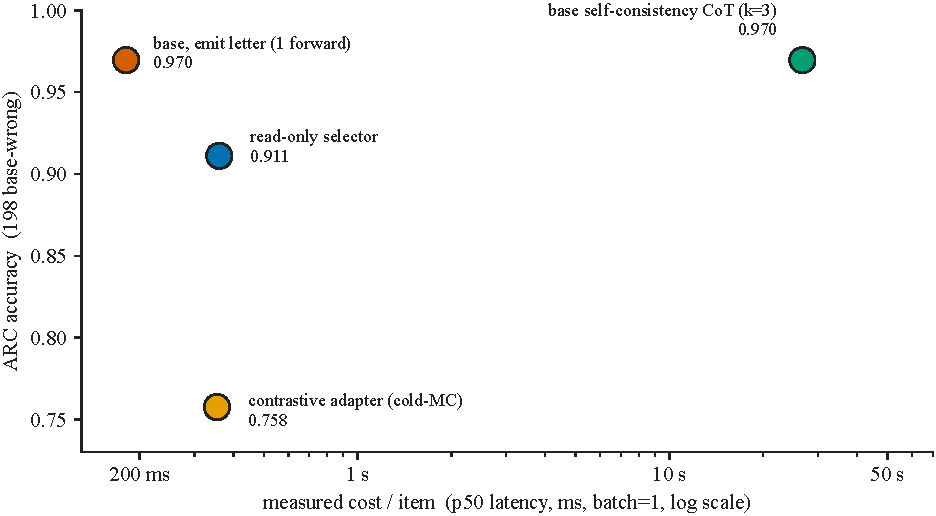
\includegraphics[width=.78\textwidth,alt={Scatter plot of the deployment triangle
on the 198 base-wrong ARC items: x-axis is measured median per-item latency at batch
one on a log scale, y-axis is ARC accuracy. Base letter-emission is the top-left
point at 0.970 accuracy and 181 milliseconds; the read-only selector sits at 0.911
and 360 milliseconds; the contrastive adapter at 0.757 and 354 milliseconds; base
self-consistency chain-of-thought far to the right at 0.970 and 26.7
seconds.}]{figures/fig_deployment_triangle.pdf}
\caption{\textbf{The deployment triangle on the 198 base-wrong ARC items, on measured
cost.} $x$: median (p50) per-item latency at batch~1, bf16, RTX PRO 6000 (log scale);
$y$: ARC accuracy. One homogeneous unit for all four routes, replacing the earlier
mixed forwards/tokens proxy --- ``one forward'' is not one unit of work, since cold-MC
scoring and the selector score every option continuation separately (${\sim}4$ per
item) while letter emission is one forward plus two tokens. Four routes: the
contrastive adapter's cold-MC scoring (0.757, 354\,ms) is dominated by everything, on
accuracy \emph{and} on cost; the read-only selector (0.911, 360\,ms) improves on it
read-only; \textbf{the base asked to emit the answer letter in one forward (0.970,
181\,ms) is both the cheapest and the most accurate route --- it matches the reasoning
baseline at ${\sim}150\times$ less latency and strictly dominates the adapter and the
selector at about half their cost}; base self-consistency CoT (0.970, 26.7\,s, 853.9
generated tokens over three traces) ties letter emission at far higher cost. The whole
LoFiT/ITI-for-cold-MC family optimizes a readout that the most trivial and cheapest
alternative --- ask the base for the letter --- already beats. \textbf{The comparison
is evidentiary, not a like-for-like scoring test:} letter emission is a different
(lettered-MCQ) readout than the cold-MC channel (\cref{method:protocol}), so the
triangle contrasts two readouts of the same base --- the lossy-readout thesis in its
sharpest form --- and the selector's role stays evidentiary (read${\neq}$write), not a
deployment recommendation, since even it is dominated by letter emission. Cost is
latency on this one accelerator at batch~1; we do not normalize FLOPs across readouts,
and batched throughput (reported in \cref{tab:triangle}) is not comparable between
prefill-bound scoring and decode-bound generation.}
\label{fig:triangle}
\end{figure}

\begin{table}[tbp]
\centering
\begin{threeparttable}
\caption{\textbf{Deployment routes on the 198 base-wrong ARC items, measured cost}
(the numeric view of \cref{fig:triangle}). Latency is median (p50) / 95th percentile
per item at batch~1, bf16, single RTX PRO 6000; tokens are generated tokens for the
generation routes and scored continuation tokens for the scoring routes. Batched
throughput is listed for completeness but is \emph{not} comparable across route
families (prefill-bound scoring vs decode-bound generation).}
\label{tab:triangle}
\footnotesize
\begin{tabular}{L{3.5cm} L{3.1cm} L{2.5cm} L{1.9cm} L{2.9cm}}
\toprule
Deployment route & ARC accuracy (198 base-wrong) & Latency p50 / p95 & Tokens /
item & Relation \\
\midrule
\textbf{Base letter-emission (1 forward, no CoT)} & \textbf{0.970} (192/198; 2
unparsed as wrong $\rightarrow$ floor) & \textbf{181 / 253\,ms} & 2.0 generated &
\textbf{cheapest \emph{and} most accurate: matches SC-CoT, strictly dominates
selector and adapter} \\
Base self-consistency CoT ($k{=}3$) & \textbf{0.970} (192/198; $k{=}5$ identical
$\rightarrow$ saturates at $k{=}3$) & 26.7 / 36.6\,s & 853.9 generated (sum over
3 traces) & ties letter-emission at ${\sim}150\times$ the latency \\
Read-only selector (\cref{disc:selector}) & \textbf{0.911} (5 probe seeds) & 360 /
479\,ms & 24.7 scored (${\sim}4$ options) & dominated by letter-emission (2$\times$
its cost, $-6$pp); Pareto-dominates only the \emph{adapter} \\
Contrastive adapter (cold-MC scoring) & \textbf{0.757} & 354 / 471\,ms & 24.7 scored
(${\sim}4$ options) & dominated by all three, on accuracy \emph{and} cost \\
\bottomrule
\end{tabular}
\begin{tablenotes}[flushleft]\footnotesize
\item \textbf{Provenance and one reconciliation.} Measured in a single harness that
re-derives every route's per-item correctness and validates it against the canonical
lm-eval artifacts before timing (\code{runs/\allowbreak e3\_\allowbreak cost/}). Within that harness the
adapter scores $0.757$ (150/198) and the base cold-MC arm $0.5025$, against $0.7626$
(151/198) and $0.5050$ in lm-eval: a one-item difference in both arms, from the
context/continuation tokenisation boundary in the re-implemented log-likelihood. The
canonical accuracies elsewhere in this paper are the lm-eval ones; the $0.757$ here is
the number produced by the same code path that produced the latencies, which is why we
report it in this table rather than silently mixing sources.
\end{tablenotes}
\end{threeparttable}
\end{table}

The selector Pareto-dominates only the \emph{adapter}; a reasoning TTC and a
one-forward letter-emission of the base both beat it --- so the whole
LoFiT/ITI-for-cold-MC family optimizes a readout that even asking the base for the
letter already beats. We therefore report the selector as \emph{evidentiary} (the
correctness signal is read-only recoverable, read${\neq}$write) and \textbf{not} as
a deployment win (dominated by letter emission at half its measured cost).
\emph{Population note (do not conflate):} the four figures here (letter-emission
0.970, SC-CoT 0.970, selector 0.911, adapter 0.757) are all on the \textbf{198
base-wrong}
subset; the selector's all-items accuracy (\textbf{0.943}, three seeds, across all
$n{=}400$ evaluation items) and the adapter's all-items accuracy
(\textbf{0.853/0.855}; \cref{tab:headline}) are computed on a \emph{different}
population and are not directly comparable to the 0.911 / 0.757 here. The 0.943 and
0.911 are the same selector on two populations, not two systems (and the canonical
lm-eval value on this subset is 0.914; the 0.911 is the same selector re-fit inside the
cost harness, see the table note). ``All items'' here
means the $n{=}400$ harness sample, \textbf{not} the full ARC-Challenge test split
--- that phrase is reserved for the R4 full-split run (\cref{sec:limitations}, ARC
acc\_norm $+36.2$).

\paragraph{read ${\neq}$ write, geometrically.}
The selector and the off-axis write together make a four-way dissociation the paper
rests on. A reader \emph{reads} correctness from the activations (selector 0.943);
an \emph{on-axis} write fails to recover the lift ($\Wknow$ 6.4\%); an
\emph{off-axis} write succeeds ($\offperp$ ${\sim}100\%$, shuffle ${\sim}0\%$,
\cref{disc:geometry}); and --- closing the loop --- the probe's decision direction
is geometrically aligned with the correctness axis it reads, \emph{not} with the
axis the adapter writes. Per head, the probe direction's signed cosine with the
functional correctness direction $\vinf$ is $+0.22$ (median $+0.20$, above the
${\sim}0.06$ null band), while its cosine with the adapter's write direction
$\thetamc$ is $|0.066|$ (at the edge of the ${\sim}0.061$ per-head null band, not
clearly within); pooled, $+0.209$ vs $|0.008|$ (clearly within the null --- the
read${\neq}$write conclusion rests on the pooled statistic). The read axis is
$\vinf$; the write axis is off-axis to it. We mark this geometric leg
\textbf{moderate, not a slam-dunk}: the alignment is 0.22 rather than 0.5,
fold-stability is 0.887 (marginal at $n \ll d = 12288$), and $\vinf$ lives strongly
on the top principal component (cos 0.55) --- but the probe reads $\vinf$ 66\%
\emph{beyond} PC1 (its PC1-routed contribution, $0.134 \times 0.55 = 0.074$, is
well under the 0.219 total), so the alignment is a genuine read, not a by-product
of dominant variance. The read ${\neq}$ write conclusion does not hinge on this leg
--- it is already carried by the probe (read), the $\Wknow$ null (on-axis write
fails), and the $\offperp$/shuffle pair (off-axis write succeeds) --- but the
geometry confirms it directionally.

\subsection{The recovery is off-axis to correctness --- of degree, on a measured
spectrum}\label{disc:geometry}

We now locate the recovery relative to the model's own correctness geometry. Per
attention head, we estimate a functional correctness direction $\vinf$ and compare
it both to the adapter's trained offset and, more carefully, to the \emph{net
effect each method has on activations}. The trained offset alone is a misleading
proxy: its whitened cosine with $\vinf$ (\cref{sec:definitions}) is $-0.003$
(within the random-direction null), it places only 6.4\% of its mass in the top
principal components (a quantity unrelated to --- and only coincidentally equal to
--- the $\Wknow$ recovery figure below), and its norm is $4.3\times$ the class gap
--- a near-orthogonal weight-space picture. But the offset is a weight-space proxy,
and a zero-cost preview of the net-effect comparison from weights alone reported
``off-axis'' (ratio ${\sim}1.05$); the clean experiment --- comparing the net
effect on activations --- refutes that simplicity.

The clean comparison yields a \textbf{spectrum}, not a single off-axis fact. A
norm-matched \textbf{random} direction (three seeds) recovers ${\approx}0\%$ of the
lift (ARC acc\_norm 0.50--0.52 ${\approx}$ base 0.505): the learned direction is
specific, not any perturbation of the right size. The strongest \textbf{on-axis}
reference we can construct locally --- a whitened Fisher-LDA direction $\Wknow$,
genuinely distinct from the mass-mean (cos with $\vinf$ 0.379) yet orthogonal to
the offset (cos with $\thetamc$ 0.0014) --- recovers only $\mathbf{6.4\%}$ of the
ARC lift (null 0.500 / adapter 0.853 / $\Wknow$ 0.522; fraction 0.064, far below
the pre-registered 0.30 kill-rule and statistically indistinguishable from zero ---
exact McNemar $p=0.136$, with the paired-bootstrap recovery CI $[-0.009, +0.136]$
and the Wilson accuracy CI $[0.474, 0.571]$ both including chance, which
\emph{strengthens} the on-axis-fails reading), and essentially nothing on
TruthfulQA; a raw mass-mean $\vinf$ recovers 11\% ($+4.0$ vs $+35.0$; $z = -6.63$).
The ordering of the two on-axis references deserves a sentence, because a reader
may suspect the smaller number was chosen for convenience: the better-constructed
discriminator ($\Wknow$, the covariance-optimal linear separator,
\cref{method:directions}) recovers no \emph{more} of the lift than the plain
mass-mean (6.4\% vs 11\%) --- improving the on-axis estimate does not improve
recovery, which is itself evidence against a knowledge-deficit account. Both
figures sit far below the 0.30 kill-rule, and the conclusion is unchanged whichever
is taken as the on-axis ceiling.

This off-axis picture does not hinge on the on-axis references being weak
estimators of the true correctness axis: the offset is off-axis \textbf{even to the
probe's own decision direction} --- the empirically optimal correctness reader ---
the in-space probe of \cref{disc:channel}, whose base-wrong AUC is 0.955 (distinct
from the \cref{disc:selector} selector's accuracy, 0.943 at $n{=}400$ / 0.914 on
base-wrong) --- at pooled cosine $|0.008|$, inside the null band (the per-head
$|0.066|$ sits at the edge of the ${\sim}0.061$ per-head null, so this upgrade
rests on the pooled statistic).

The two \emph{methods}, measured by net activation effect, are both \textbf{mostly
off-axis} --- the contrastive adapter at cosine 0.088 (ratio 1.74 vs a random
direction) and generic SFT at cosine 0.199 (ratio 3.93) --- but generic SFT is
$\mathbf{2.3\times}$ \textbf{more on-axis} than the contrastive adapter. The
recovery is thus off the correctness axis \emph{to a degree that depends on the
method}: random ${\approx}0\%$ (cos${\approx}0.05$, ratio 1.0) $\rightarrow$
$\Wknow$ 6.4\% (the on-axis reference) $\rightarrow$ generic SFT ${\sim}62\%$ (cos
0.199, ratio 3.93) $\rightarrow$ contrastive 100\% (cos 0.088, ratio 1.74). Note
the two orderings are deliberately \textbf{not} monotone in each other: recovery
fraction and on-axis-ness are different axes of the spectrum (the most off-axis
direction, random, recovers nothing; the more on-axis method, generic SFT, recovers
\emph{less} than the contrastive one) --- the spectrum is a two-axis object, not a
single scale.

This refines the earlier ``purely off-axis'' framing into the central figure of the
paper, and it is consistent with the earlier finding that the two functional
correctness faces are themselves co-located (whitened cosine $\vinf{\cdot}\vret$
$+0.283$, BCa95 $[+0.276, +0.291]$, null ${\pm}0.007$, $n{=}316$ heads): the
recovery is off the shared correctness substrate by a method-dependent amount, not
aligned with either face of it.

This co-location appears to sit in tension with work reporting that recall and
reasoning occupy \emph{causally separable} circuits
\citep{DisentanglingRecallReasoning}: if the correctness faces share a substrate,
separately ablating recall and reasoning should not be possible. The tension
dissolves at the level of description, because the two results measure different
objects. That work measures task-circuit separability (in Qwen and LLaMA): ablating
one functional circuit leaves the other intact, ``separable but interacting.'' We
measure the \emph{direction of a trained offset} relative to the functional
correctness direction, in Gemma~4 31B IT. A substrate can host circuits that
partition sufficiently for separate ablation \emph{and} carry functional directions
that are co-located, with our $+0.283$ measurement living in that work's
``interacting'' seam rather than denying its separability. Our novel layer is
neither: the direction the adapter actually moves is off-axis to both functional
faces, which is why a partition-based account of the spillover --- and the hope of
re-selecting heads to avoid it --- does not hold.

\paragraph{A direct causal decomposition: the off-axis push is privileged, not any
perturbation of the right size.}
The spectrum above is read from each method's net activation effect; a second, more
direct experiment decomposes the adapter's \emph{own} offset against the
correctness direction and asks which component carries the lift. We split the
trained offset, per head, into a component parallel to the functional correctness
direction ($\offpar$) and a component perpendicular to it ($\offperp$), and inject
each through the identical recovery harness used for every arm above, at its
natural norm from the decomposition ($\offpar$ is consequently ${\sim}16\times$
smaller in norm than the $\Wknow$ arm --- the equal-norm control inside the
perpendicular complement is the shuffle arm below, norm-matched per head to
$\offperp$).

The perpendicular component recovers essentially all of the lift (ARC acc\_norm
0.8525, ${\sim}100\%$; HellaSwag, Winogrande, TruthfulQA 99--104\%), while the
parallel component recovers none (ARC acc\_norm 0.505 = the Gate-A base exactly,
0\%; raw acc 0.5025). Given $\cos(\thetamc, \vinf) \approx -0.003$, $\offperp$
${\approx}$ the full offset by construction; the informative arms are $\offpar$ (an
on-axis push at the offset's own scale does nothing) and the shuffle (equal-norm,
same subspace, learnedness as the only variable).

Because the \emph{same} harness that yields 100\% for the perpendicular push yields
only 6.4\% for the on-axis $\Wknow$ reference, the on-axis failure is a real
property of the geometry, not an insensitivity of the injection method --- the
harness is direction-sensitive. This closes the non-identifiability objection
\citep{NonIdentifiability} on the \emph{harness} side.

We close it on the \emph{write} side as well: a random direction sampled inside the
\emph{same} perpendicular complement, norm-matched per head to $\offperp$ (sanity
check: $|\cos|$ to $\vinf$ ${\approx}$ $5\times10^{-17}$, $|\cos|$ to the learned
$\offperp$ ${\approx}$ $0.047 \approx 1/\sqrt{256}$), recovers ${\sim}0\%$ of the
lift across three seeds (ARC fraction $-0.04$ / $-0.01$ / $-0.01$; the lone
non-zero, Winogrande ${\sim}12\%$, is a small lift in noise) against $\offperp$'s
${\sim}100\%$. Same harness, same norm, same subspace --- the only variable is
\emph{learnedness} --- so it is the learned structure \emph{inside} the off-axis
complement that lifts, not orthogonality-plus-norm. Following the recommended
rebuttal template of comparing a learned direction against a random one
\citep{ConfidenceManifold}, both orthogonal controls (the on-axis reference and the
shuffled perpendicular) have an effect on the lift indistinguishable from zero
while the learned off-axis push does not; and reported specificity failures of
activation directions are \emph{cross-model}, whereas within-model --- our setting
--- directions remain specific \citep{SyedActivationDirections}, so that result
does not subsume this control.

(These two ``off-axis'' readings are not in tension: $\offpar$ 0\% is a
decomposition of the trained offset in \emph{weight space}, whereas the cosine
0.088 is the \emph{net effect on activations} --- different objects on different
metrics, both saying the on-axis component does not carry the lift.)

A norm $4.3\times$ the class gap also invites the question whether a linear
on/off-axis decomposition is still meaningful at the offset's operating point. The
dose--response sweep (\cref{disc:pathologies}) is the empirical check: the response
to scaling the offset over $s \in [0, 1]$ is smooth and monotone --- the scoring
lift saturates, then the generation damage onsets --- with no discontinuity or
chaotic regime anywhere on the axis, so the injection operates on a graded response
surface where the decomposition is interpretable. We nonetheless scope the
geometric claims to the trained offset at its trained scale rather than asserting
magnitude-invariance.

A training-time constructive control closes the causal argument from the other side
(necessity, complementing this sufficiency): an on-axis training penalty toward
$\vinf$, swept over $\lambda$, does \emph{not} rescue transfer at matched lift
(fork (b), \cref{sec:open}) --- so the $+35$ is the off-axis mass by necessity, not
only by construction. Together, the $\offperp$/random spectrum (sufficiency) and
fork (b) (necessity) make the off-axis reading a two-sided causal claim.

\subsection{No single-layer locus: the lift scales with total offset magnitude}
\label{disc:locus}

The recovery has no causal layer locus. Across a layer-band patching sweep, the
recovered fraction correlates with the \emph{total magnitude} of the learned offset
($\Sigma|r|$) at \textbf{0.985}, far more than with the number of heads patched
(0.832). (We read this as \emph{no single-layer locus} rather than a strict
magnitude-over-head-count causal claim: 0.985 and 0.832 are coupled correlations
from the same band sweep, not a test that isolates magnitude from head-count; what
the sweep licenses is that no privileged layer repairs the readout, not a proof
that head-count is causally inert.) The natural temptation --- to read ``layers
36--40 carry 87\% of the lift'' --- is a head-count artifact: that band simply
contains 71\% of the adapter's heads (which span L30--55). There is no privileged
layer at which the lossy readout is repaired; the recovery is a property of the
aggregate magnitude of an off-axis-of-degree push distributed across heads,
consistent with the over-scaled offset (\cref{disc:geometry}) and the coherent-sum
logit signature (\cref{disc:pathologies}).

\subsection{The deployment pathologies are coupled to injection, not to the lift}
\label{disc:pathologies}

Recovering the lift the contrastive way introduces two deployment costs --- no
transfer to generative CoT (a mechanistic breakage of multi-step reasoning) and
retrieval/recall spillover. (A third cost we previously listed --- an end-of-turn
``collapse'' --- is retracted at the end of this section as a measurement
artifact.) A clean control shows the two surviving costs are coupled to \emph{how}
the offset is injected, not to the lift as such. The generic Align-LoRA that
recovers most of the lift (\cref{disc:inducibility}) \textbf{preserves generation}:
gsm8k $0.96{\rightarrow}0.95$ (n.s.), where the folded contrastive offset destroys
it (gsm8k ${\rightarrow}0.17$ baked, and $-25\pp$ adapter-applied; below).

The retrieval spillover, in turn, is consistent with the off-axis push landing on
\textbf{retrieval-load-bearing heads} --- the adapter's heads overlap heads that
carry retrieval (in the D.1 SocialIQA adapter: MMLU $-19.59\pp$, unrecovered by
sparsity tuning from K=24 to K=12; correlational, per-head causal test pending). We
keep this head-level overlap claim distinct from the \cref{disc:geometry} finding
that the two functional correctness \emph{faces} are co-located (cos
$\vinf{\cdot}\vret$ $+0.283$): face co-location implies that re-selecting heads
within the same band cannot dodge the retrieval substrate, but it does \textbf{not}
assert that the adapter's off-axis direction aligns with $\vret$ --- by
\cref{disc:geometry} the offset is off-axis to \emph{both} faces, so the spillover
is an off-axis perturbation disturbing a shared substrate, not the lift being
projected onto the retrieval face. The pathologies are therefore the downstream
shadow of folding an off-axis-of-degree perturbation into the weights, not an
inevitable price of the lift: a different injection (generic SFT) recovers much of
the lift without them.

A \emph{third} injection mode confirms the coupling from the other side: blending
the offset in at \textbf{decode time} at reduced strength --- a milder intervention
than folding it into the weights --- still buys no generative transfer. Sweeping
the blend coefficient $\varepsilon$ on gsm8k ($n{=}100$,
$\varepsilon \in \{0, 0.2, 0.5, 1.0\}$), no interior $\varepsilon$ beats the base
by more than noise (base 0.97; $\varepsilon{=}0.2 \rightarrow 0.98$,
$\varepsilon{=}0.5 \rightarrow 0.99$, both within 1--2 items of base at $n{=}100$
and under the pre-registered 2pp window), while full-strength decode-time injection
($\varepsilon{=}1$) reproduces the loss (0.87, $-10\pp$) --- there is no transfer
window, so the off-axis lift is not deployable to generation even as a decode-time
steering vector. (Its $\varepsilon{=}1$ $-10\pp$ is milder than the $-25\pp$ of the
fully-baked adapter --- the blend harness perturbs a subset of heads at generation
only --- so we read it qualitatively, not as a magnitude.) Even at
$\varepsilon{=}1$ the end-of-turn rate stays at 0.97, independently corroborating
the retract below: the generative cost is degraded reasoning, not a failure to
terminate.

The contrastive adapter's generative loss on gsm8k is itself a mechanistic loss,
not a truncated chain of thought. Run generatively under an apples-to-apples
protocol (chat template on, 5-shot, $n{=}400$), the adapter scores \textbf{0.7275}
strict-match against the base's \textbf{0.9775} ($\mathbf{-25\pp}$; R6, the
canonical kill-rule run, with an earlier provisional R6probe agreeing at $-24\pp$).
That gap is \textbf{flat across a generation-budget sweep}: 0.7275 at caps
\{512, 2048\} (R6probe: 0.7375 flat at \{512, 1024, 2048\}), with the base
\textbf{byte-identical} across caps. The base's reasoning runs well under the
smallest cap, so the cap never bites it. Turning off the chat template only makes
the gap \emph{worse} (base 0.730 / v7mc 0.035, $-69\pp$): both arms degrade, so the
template-ON apples-to-apples figure is the canonical one. The $-25$ is therefore
not a template artifact.

The adapter \emph{does} consume the larger budget --- 26/400 of its generations
grow with the cap --- yet \textbf{0/400 documents change strict verdict}. A
forensic split of the 105 strict failures at cap 2048 separates the two failure
modes: \textbf{79} are clean-wrong (they emit a \code{\#\#\#\#} answer with the
wrong number --- reasoning resolved but defective, independent of the cap), and the
remaining \textbf{26} are genuine non-terminating \emph{reasoning} loops (a real
task-specific failure, distinct from the retracted factual-recall artifact below)
\emph{already} present at cap 512 (e.g.\ doc 88: a ``\ldots not sold by
Harald\ldots'' loop filling the budget, no \code{\#\#\#\#}), i.e.\ the failure
\emph{precedes} the budget rather than being caused by truncation.

The $-25\pp$ is therefore a mechanistic breakage of the reasoning chain --- coupled
to the contrastive injection, consistent with \cref{disc:arbiter}'s no-transfer ---
not a measurement artifact of a clipped CoT. These 26 loops are a
\emph{task-specific} reasoning failure on gsm8k, \textbf{not} evidence of a general
termination collapse (which the corrected re-measure below refutes on direct
recall).

(We retain the gsm8k caveat: it is OOD and does not measure in-domain transfer, so
it bounds the \emph{collateral} claim, not the no-transfer claim of
\cref{disc:arbiter}.)

\paragraph{The dissociative triangle.}
Three facts about the contrastive adapter's generative behaviour dissociate, and we
state them together because the gsm8k loss could otherwise be read as a blanket
generative failure. (a) \emph{Direct factual recall is clean:} on single-hop recall
the adapter terminates at 100\% and answers tersely and correctly --- the earlier
$48{\rightarrow}4\%$ / $60{\rightarrow}4\%$ ``collapse'' is a \textbf{retracted}
eos-token measurement artifact (below). (b) \emph{Multi-step reasoning is broken:}
on gsm8k the adapter loses $\mathbf{-25\pp}$, a mechanistic breakage (flat across a
generation-budget sweep; 26 non-terminating reasoning loops already present at cap
512), not truncation and not a termination failure. (c) \emph{The damage is coupled
to injection, not to the lift:} the generic SFT that recovers most of the lift
preserves gsm8k ($0.96{\rightarrow}0.95$), and the reasoning loss is reproduced
across \textbf{four independent injection modes} --- folded/baked ($-25\pp$),
decode-time blend ($\varepsilon{=}1$, $-10\pp$), activation-scale steering (damage
confined to the $0.75{\rightarrow}1.0$ band), and confirmed from the other side by
the Align control that recovers the lift \emph{without} the loss --- so it is a
property of \emph{how} the offset enters the weights, not of the lift.

\textbf{A confound we state rather than hide:} the (a)-clean-vs-(b)-broken contrast
conflates two things --- multi-step \emph{reasoning} and \emph{distribution
distance} (gsm8k is OOD to the tqa+arc training) --- so gsm8k bounds the
\emph{collateral reasoning cost}, not the no-transfer claim. The no-transfer per se
does \textbf{not} rest on gsm8k: it is carried by the per-item arbiter (the fixed
ARC items sit at the base's CoT ceiling, 124/124, \cref{disc:arbiter}) and by the
out-of-task GPQA cold-MC lift ${\sim}0$ while base GPQA CoT is 0.71
(\cref{results:arbiter}). gsm8k carries only the \emph{collateral damage to
reasoning}, and that damage is the triangulated four-injection-mode result above.

\paragraph{The collateral reasoning loss is dose-separable from the scoring
benefit --- in steering, not in the baked adapter.}
The $\varepsilon$-sweep above varied a decode-time \emph{blend} of one face; a
cleaner test places both faces on a \emph{single} magnitude axis by scaling the
injected offset itself (activation-scale $s \in \{0, 0.25, 0.5, 0.75, 1.0\}$;
$s{=}1$ reproduces the adapter's scoring lift --- ARC acc\_norm
$0.505{\rightarrow}0.855$, $+35.0\pp$ ${\approx}$ the baked $+35$, raw acc 0.5025).
On this common axis the two faces cross their thresholds at \emph{different} doses:
the scoring benefit \textbf{saturates early}, reaching its full value already at
$s{=}0.75$ (ARC 0.855, identical to $s{=}1.0$), while the gsm8k reasoning score
holds at base through $s{=}0.75$ ($0.970{\rightarrow}0.950$, at the edge of the
pre-registered 2pp window) and drops only in the $0.75{\rightarrow}1.0$ band
($\rightarrow 0.815$). The scoring-benefit threshold thus lies \emph{below} the
reasoning-harm threshold, so the $0.75{\rightarrow}1.0$ magnitude is collateral
damage with no accompanying scoring gain (the lift is already at ceiling).

This does \textbf{not} reopen a transfer window. We are careful with the wording,
because two interior points of the $\varepsilon$-sweep above do print
\emph{numerically} over base ($\varepsilon{=}0.2 \rightarrow 0.98$ and
$\varepsilon{=}0.5 \rightarrow 0.99$ against base 0.97): at $n{=}100$ those are
one- and two-item differences, inside the pre-registered 2pp window, so we read
them as noise and not as a gain --- no dose produces a reasoning improvement we
would defend, but the honest statement is ``no dose rises above base beyond
noise,'' not ``no dose rises above base.'' What is dose-separable is the
\emph{collateral damage}, not a deployable gain. The separation is a property of
the \textbf{injected, scaled offset (steering); the $-25\pp$ headline is the
fully-baked adapter at $s{=}1.0$}, so whether a \emph{trainable} adapter can be
held in the low-damage regime is an open question, not a result here (the
$s$-swept gsm8k figures use the steering harness, $n{=}200$, and are read as curve
\emph{shape}, not against the canonical $-25\pp$).

We name one prior-art foil directly: an angle--norm account of steering
\citep{AngleNorm} predicts on geometric grounds that a concept-discriminative
(angular) readout should saturate at lower magnitude than generative coherence
(norm-sensitive) breaks --- so a reviewer may read our dose separation as
geometrically expected. We distinguish it on three measured grounds that account
does not cover: the offset is \textbf{off-axis} to the concept direction
(\cref{disc:geometry}, not an on-concept angular push), its mechanism is
\textbf{non-linear} (the direct-logit reading under-reads it,
\cref{disc:negatives}), and it is \textbf{not a norm/temperature rescaling}
(cosine with the temperature direction 0.023, \cref{disc:negatives}) --- so the
separation here is not the generic angular-saturates / radial-breaks story, and we
report it as a dose-refinement of the \emph{collateral cost}, not as a deployable
window.

An independent result in a different regime corroborates the \emph{shape} of this
dissociation from the write side. A budget-normalized \textbf{control-window} law
for single-neuron steering \citep{LeverageIsNotReach} finds that coherent
behavioral control saturates below a \textbf{collapse ceiling}, and --- its titular
point --- that \emph{leverage is not reach}: a single neuron can flip a behavior's
readout face (e.g.\ bypass refusal) in fluent, on-task text while genuine
downstream reach appears only later and only for a subset of pivots (three of six
audited). That is the single-neuron analogue of our dissociation --- control of the
\emph{scoring} face at a dose below where generative coherence breaks, with the
scoring gain never buying generative reach (\cref{disc:arbiter}) --- obtained in an
unrelated setting (sparse behavior-gating neurons, not a multi-head correctness
offset), so we read it as convergent support for the threshold structure, not as
the same experiment.

\paragraph{A previously-claimed end-of-turn collapse is retracted as an eos-token
artifact.}
We earlier reported that the contrastive family collapses end-of-turn termination
(V7-mc / D.1 factual $48\%{\rightarrow}4\%$, social $56\%{\rightarrow}4\%$, an
analogous V7-mc $60\%{\rightarrow}4\%$). That is a measurement artifact: the
verbosity harness (\code{eval\_\allowbreak adaptive\_\allowbreak verbosity}) scored termination on the base
\code{<eos>} token, whereas Gemma~4 closes a conversational turn with
\code{<end\_\allowbreak of\_\allowbreak turn>} (token 106). With the corrected turn-stop token, base
factual termination is \textbf{100\%} (reported 48\%) and the contrastive adapter's
factual termination is also \textbf{100\%} (reported 4\%) --- there is \emph{no}
collapse; the adapter's factual answers are correct, terse, and terminate
(``Paris'', ``Au'', ``1945''), and the ``degenerate loop'' read earlier in this
\emph{factual-recall} smoke was junk generated \emph{after} the
\code{<end\_\allowbreak of\_\allowbreak turn>} the harness had failed to stop on --- a measurement
artifact, distinct from the genuine gsm8k \emph{reasoning} loops above.

The honest reframe is that the contrastive adapter \textbf{does direct factual
recall} (terse, correct, terminating --- no degradation vs the base, which is also
correct but verbose) and \textbf{breaks multi-step reasoning} (gsm8k $-25\pp$) ---
which fits the per-item arbiter (\cref{disc:arbiter}: the fixed items are knowledge
the base reaches by \emph{reasoning}) and the no-transfer result better than a
blanket ``cannot terminate'' claim did.

The analogous D.1 figures were re-measured: the ${\rightarrow}4\%$ ``collapse'' is
withdrawn, but a real, modest termination degradation remains on open-ended
generation (social $96{\rightarrow}76\%$, creative $68{\rightarrow}12\%$) ---
adapter-dependent and off the V7-mc headline; this paper makes no
${\rightarrow}4\%$ termination-collapse claim.

\subsection{Mechanism candidates ruled out: not temperature, not token-frequency
(a content/symbol signpost)}\label{disc:negatives}

Two mechanistic accounts of the offset are ruled out, and one is left as a
signpost; the exploratory workspace and generation-face analyses that extend this
section are collected in \cref{app:mechanism} and carry no claim here.

\paragraph{Not a temperature / null-space mechanism.}
A natural hypothesis, given the readout framing, is that the offset acts like a
confidence-regulation / entropy neuron --- writing into the unembedding null space
to rescale the logit temperature without re-ordering the argmax
\citep{ConfidenceRegulationNeurons}. It does not. A direct-logit decomposition
projects the residual write onto the \emph{genuine} temperature direction
$d^{*} = \arg\min\|W_U r - \mathbf{1}\|$ (whose own logit image is 0.9988 uniform,
so it is well identified) and finds cosine \textbf{0.023} --- orthogonal to
temperature at chance level (random-direction baseline
${\sim}1/\sqrt{d_{\mathrm{model}}} \approx 0.014$). Causal activation-patching at
the scoring positions where the lift lives (the option-continuation tokens)
confirms it: the \textbf{relative} temperature fraction is only \textbf{0.215}
(CI\textsubscript{hi} 0.224 ${\leq}$ the pre-registered 0.35 kill-rule; in absolute
fractions of the effect, temperature 0.177 / ranking 0.803), so the offset re-ranks
rather than rescales --- it moves logit \emph{differences}, not their mean.
\emph{Position matters:} at the next-token generation position the offset flattens
the distribution more (temperature fraction 0.38), so the negative is anchored at
the scoring positions. (Full decomposition --- the $d^{*}$ identification, the
anisotropy caveat on the raw uniform-shift fraction, the causal cosine $-0.149$,
and the linear-attribution-under-reads-the-off-axis-alignment pattern
\citep{LeverageIsNotReach} --- in \cref{app:mechanism}.)

\paragraph{Not a token-frequency edit; a content/symbol signpost.}
Direct-logit attribution over the 48 heads finds \textbf{no clean lexical
mechanism}; the one robust signature is on the \emph{suppression} side --- single
uppercase letters, punctuation and structural tokens, exactly the surface tokens of
multiple-choice labels and turn formatting --- the readable face of the
\emph{format-preference} channel that aligned-model calibration distinguishes from
answer-decision uncertainty \citep{AlignedMCCalibration}. The most promising
unifying candidate is the content/symbol-binding channel MCQA mechanism work
isolates \citep{TwoStageMCQA,CorrectLetterHeads}, but the decisive TEXT-vs-LABEL
scoring ablation is \textbf{consistent-with, not clean}: on ARC the label-arm lift
survives a headroom normalization ($\Delta_{\mathrm{letter}}$ $+0.1575$ raw /
$+0.17$ norm) yet the permutation controls that would isolate letter-specificity
are ceiling-starved, and on TruthfulQA the letter arm is itself at ceiling
(uninformative). We report the symbol channel as a signpost, not a named mechanism.
The symmetric cosine test for this third candidate --- the same construction
standard the temperature and frequency negatives received --- has now run: a
\emph{mean} structural-token contrast direction (the readout-row difference of
means between the ${\sim}27$k structural tokens and the rest; exact by
construction, and its logit image separates the classes cleanly) has cosine
$\mathbf{-0.0099}$ with the offset's aggregate write ($\mathbf{-0.0115}$ for the
uppercase-letter-only variant), at the null floor ($1/\sqrt{d} \approx 0.014$,
$3\times$-null gate 0.041) like the other two; a \emph{full-target} format
direction is not linearly identifiable in the unembedding basis at all
(identification $r = 0.78 <$ the 0.9 self-gate that $d_{\mathrm{freq}}$ passed),
consistent with the suppression signature living in the \emph{tail} of the offset's
logit image rather than in its mean --- which is exactly why the channel stays a
signpost: the offset is not the mean format direction either
(\code{runs/\allowbreak oq1\_\allowbreak functional\_\allowbreak axis/\allowbreak format\_\allowbreak control.\allowbreak json}). The \emph{other} Stolfo
component --- a token-frequency edit --- is \textbf{closed at the attribution
level}: over the full wikitext-103 corpus (121.6M tokens) the recovered frequency
direction is identified at $r{=}\mathbf{0.906}$ (past its 0.9 self-gate) and the
offset's cosine with it is \textbf{0.0128} (at the null floor, below the
$3\times$-null gate 0.041), so the offset is not a token-frequency edit. One scope
note travels with it: unlike the temperature negative, the frequency control had
not received a causal-patching cross-check --- and the temperature case showed the
causal alignment can exceed the linear read severalfold
($0.023 \rightarrow -0.149$) --- so we ran that cross-check rather than assume it.
It comes back \textbf{negative for a sign-flip}: projecting the real
base${\rightarrow}$adapter logit delta onto the frequency signature gives cosine
$\mathbf{+0.0059}$, CI $[-0.0027, +0.0142]$ --- same sign as the direct-logit
0.0128, smaller ($\times0.46$), and crossing zero --- where the temperature case
flipped sign and grew sixfold ($0.023 \rightarrow -0.149$, CI $[-0.158, -0.140]$).
The sharpest contrast is in sign \emph{consistency} rather than magnitude: the
per-item frequency projection has comparable mean absolute size to the temperature
one (0.120 vs 0.177) but inconsistent sign (66\% positive, against 99\% for
temperature), and a component whose sign varies item-to-item cannot be the
mechanism of a lift that is systematic across items. One limit travels with the
negative: the frequency direction \emph{orthogonalized against the base logits} ---
the part of log-frequency not already shared with the temperature channel, which
has no direct-logit counterpart --- does carry a small but non-zero causal
component (cosine $\mathbf{+0.0298}$, CI $[+0.0221, +0.0374]$, ${\sim}1/5$ of the
temperature component and ${\sim}1/27$ of the ranking one). Frequency is therefore
ruled out as the \emph{mechanism}, not as a trace contaminant.

An exploratory Jacobian-lens analysis (single seed) further places $\thetamc$
\emph{off} the model's global workspace --- an automatic-channel edit, the
mechanistic shape a direction that lifts cold scoring but does not transfer to
reasoning should have --- and an nnsight causal patch on real generation positions
finds the same structure-suppression signature (${\sim}91\%$ structural, a
$\times3$ enrichment); we report both, and the per-position recall-tail resolution,
in \cref{app:mechanism} and rely on them for no claim above.

\subsection{What the offset does do: it rescales the decision margin with two global
scalars, not item by item}\label{disc:mechanism}

Having ruled temperature and frequency out, we can say what the arms \emph{do} change,
and it is a global property of the score distribution rather than an item-by-item
judgement. Write the per-item decision margin as
$g = \log p(\mathrm{gold}) - \log p(\mathrm{best\ distractor})$ and compare an arm's
margins against the base's on the same items. One scope note belongs here rather than
in a footnote: $g$ is a \emph{gold-relative} coordinate, so everything below describes
how the arms move a margin defined using the label. It does not assert that the
underlying edit is computed without the label --- what is item-independent is the
\emph{description}: two scalars per cell, constant across items, no per-item term.
(An affine map applied to the raw option scores could not change any $\arg\max$ at
all; it is precisely because the intercept acts on the gold-relative margin that
accuracy moves.) The ratio
$\mathrm{sd}(g_{\mathrm{arm}}) / \mathrm{sd}(g_{\mathrm{base}})$ splits the eighteen
arm${\times}$task cells we have, across both families, without exception:
\textbf{the contrastive objective in domain expands the margin scale}
($2.10 / 1.50 / 1.95$ on ARC / HellaSwag / TruthfulQA in Gemma,
$1.47 / 1.63 / 1.81$ in Qwen) and \textbf{everything else compresses it} to
$0.41$--$0.72$ --- ordinary cross-entropy in either domain, and the contrastive
objective itself once trained out of domain ($0.63$--$0.70$). That last cell is worth
stating precisely: out of domain the objective keeps an accuracy advantage over plain
cross-entropy at identical parameterization and corpus, but it lands on the
\emph{compressing} side of the split, losing the scale signature that in-domain
training produces.

Scale is one scalar; the accuracy change needs a second, which is where the rescaled
distribution sits relative to zero. Fitting
$g_{\mathrm{arm}} \approx a\,g_{\mathrm{base}} + c$ per cell and reading off the
effective decision threshold $-c/a$, the shift is large and negative wherever the arm
helps (Gemma contrastive: $-43.6 / -24.7 / -47.1$ nats) and positive wherever it hurts
(both plain-CE arms on TruthfulQA, $+4.2$ and $+11.8$). Its \emph{sign} matches the
sign of the measured accuracy change in 17 of the 18 cells; the exception is the one
cell whose measured effect is itself null ($+0.8\pp$, a no-op in 2 of 3 seeds). Pushed
all the way, a deterministic map built from those two global scalars alone --- carrying
no information about which item is which --- reproduces the direction and rough size of
every accuracy change with a non-zero effect to reproduce (17 of 18; the eighteenth
measures exactly zero), over-explaining by a median of $29\%$, cell-wise range
$0.70$--$1.93\times$ the measured effect. We report that as sufficiency of \emph{form},
not as a calibrated fit: the map is deterministic where the real arm is noisy, and
noise attenuates.

Because that fit is in-sample, we re-ran it \emph{out of sample}: the two scalars are
estimated on a random half of the items and used to reproduce the accuracy change on
the held-out half, 200 splits per cell. The map survives, and in fact tightens ---
the median over-explanation falls from $29\%$ in-sample to $\mathbf{16\%}$ held-out,
and the three cells carrying the canonical contrastive effect are unchanged to two
decimals (ARC $1.43 \rightarrow 1.42$, HellaSwag $1.14 \rightarrow 1.16$, TruthfulQA
$1.29 \rightarrow 1.28$). Sixteen of eighteen cells keep the sign of the measured
effect out of sample; the two that do not are the cells whose measured effect is
$+0.8$ and $+2.3\pp$, where the ratio divides by a denominator near zero. Part of the
in-sample over-explanation was therefore fitting noise, and none of the load-bearing
cells depend on it (\cref{app:mechanism}).

The obvious objection is that the arms might rescale \emph{and} aim, so we bound the
aiming rather than assume it away. The tempting null --- permuting each arm's per-item
push across all items --- is invalid here, because any rescaling makes that push
$(a-1)\,g_{\mathrm{base}} + c$, anticorrelated with the base margin by construction and
without any knowledge of which option is correct; such a null therefore rejects for
every arm that rescales, which is all of them. Permuting instead \emph{within strata of
the base margin} preserves the conditional law of the push and destroys only item
identity, and under it 1 of 18 cells exceeds $2\sigma$ where the invalid control gave
9 of 18. The survivor does not hold up: selected post hoc from 18, it fails both
Bonferroni and BH-FDR ($p = 0.0066$ against a threshold of $0.00278$), and its
significance rides on a free parameter --- $z$ runs from $1.30$ to $3.43$ as the
stratum width goes from 10 items to 100. Its residual does differ from zero under a
paired bootstrap ($+1.12\pp$, CI $[+0.20, +2.09]$ at a stratum width of 25), so an
item-specific component exists in that cell. We decline to quote a single number for
its size, because the same free parameter moves it: the residual runs
$+0.28 / +1.31 / +1.66 / +3.12\pp$ as the stratum width goes from 10 to 100 items,
i.e.\ between ${\approx}1\%$ and ${\approx}14\%$ of that cell's $+22.7\pp$ effect, with
no width privileged a priori. The conservative reading is therefore that any
item-specific component in the most favourable of the eighteen cells is bounded by
roughly a seventh of the effect, and the item-independent rescaling accounts for the
rest. We take that as the ceiling, not as an estimate.

This is the readout thesis made mechanical, and it accounts for the task pattern
without new machinery. ARC sits on the edge of its own decision boundary --- median
$|g|$ of $9.8$ nats in Gemma and $8.5$ in Qwen against $17$--$23$ on HellaSwag and
TruthfulQA, with $12.5\%$ and $22.2\%$ of its items inside 3 nats --- so a global
rescaling carries more items across zero there than anywhere else. (Density alone does
not order the finer structure: in Gemma, HellaSwag at $7.0\%$ and TruthfulQA at
$7.25\%$ are tied while their effects differ, so we report it as a descriptor and not
a predictor.) An edit that moves a threshold need not know which questions it is
fixing, which is why the items it fixes turn out to be ones the base could already
reach by reasoning (\cref{disc:arbiter}), and why the same push has nothing to offer a
generation channel that never scores the options against each other at all.

Three limits travel with this. It is measured on raw accuracy throughout, which is the
right scale for a mechanism stated in log-probability differences but is \emph{not} the
metric behind two of the four headline lifts (\cref{lim:metric}); the two are not
interchangeable. The contrastive-canonical cells are a single training run --- the
published adapter --- while the plain-CE cells carry three seeds each. And the
stratified null does not show that the arms carry no per-item information; it shows
that this statistic cannot distinguish such information from a rescaling, with the
audit above bounding what it could be hiding.

\subsection{Two failure modes: ARC carries the readout story (suppression),
TruthfulQA is answer-prior (promotion)}\label{disc:heterogeneity}

The readout account is established on ARC and must not be read across all tasks
uniformly. On \textbf{ARC}, the lift is question-conditional: a PMI /
decision-conditional control retains \textbf{78\%} of it (naive $+0.3275$
$\rightarrow$ PMI $+0.2550$), and the choices-only lift is only $+0.0375$ (CI
$[-0.005, +0.08]$, not clearly positive) --- so it is genuine,
question-conditional, and the case the \cref{disc:arbiter} arbiter and
\cref{disc:geometry} spectrum characterize. On \textbf{TruthfulQA}, by contrast,
much of the $+37.25$ is an \textbf{answer-prior / surface-form Goodhart} effect:
the choices-only lift is $+0.2225$ (CI $[+0.1675, +0.2725]$) and the adapter
selects the correct option \textbf{0.5725 of the time with no question at all}
(base 0.35, chance 0.229); PMI retains 68\%. This matches known multiple-choice
shortcut behavior in which highest-probability scoring favors options by surface
form independent of the premise \citep{SurfaceFormCompetition}, and choices-only
accuracy sits above chance \citep{ChoicesOnlyCheater}.

The two tasks also fail the cold readout by \textbf{opposite calibration
mechanisms}, visible in the base gold-rank distribution on the items the adapter
flips. On \textbf{ARC} the gold is \textbf{suppressed} --- buried at median rank 2,
with only 46\% of flipped items having it at rank 1 --- so the adapter must
\emph{promote} it past more fluent distractors (gold-mass added 0.35 $>$ wrong-mass
removed 0.21). On \textbf{TruthfulQA} the gold is instead a \textbf{flat
near-miss}, already at median rank 1 (51\% of flipped items at rank 1), so the
adapter mostly nudges an already-near-top answer over the line. TruthfulQA is
therefore not merely ``excluded from the inducibility control'' --- it is a
\textbf{second failure mode} of the same lossy readout (a near-miss the
answer-prior resolves), distinct from ARC's active suppression. We report
TruthfulQA held-out, as evidence the scoring lift is \emph{real} and exploitable,
not as evidence for the readout mechanism, which rests on ARC. The paper-level
rule: the lift is not a single phenomenon --- TruthfulQA is answer-prior
(promotion); ARC is question-conditional, off-axis-of-degree, and non-transferable
(suppression).

We scope the TruthfulQA result precisely. It was previously a pre-registered hedge
--- a selection lift on the mc1 metric ($+37.25$, paired-significant under exact
McNemar, Holm-corrected $p_{\mathrm{corr}}$ $6.26\times10^{-38}$, b=6/c=155)
pending a held-out-plus-mc2 control --- and that control has now \textbf{run} (full
set, $n{=}817$), removing the hedge in a specific way. The lift \textbf{generalizes
held-out}: on the ${\sim}20\%$ never matched into training (164 UNSEEN of 817),
the v7-mc gain is $\Delta_{\mathrm{UNSEEN}}$ mc1 $\mathbf{+37.8}$,
indistinguishable from $\Delta_{\mathrm{SEEN}}$ $+36.9$, and it holds on the second
metric ($\Delta_{\mathrm{UNSEEN}}$ mc2 $\mathbf{+26.1}$) --- clearing the
pre-registered gate ($\Delta_{\mathrm{UNSEEN}}$ mc1 ${\geq}+15\pp$ and $\Delta$mc2
${>}+10\pp$) comfortably. So the $+37.25$ is \emph{not} memorization of
train-on-eval pairs (the matched corpus covers ${\sim}79.9\%$ of the eval, yet the
held-out gain is undiminished), and it is real beyond the mc1 selection metric. The
decisive contrast is with the generic control: the higher-capacity Align-LoRA, which
recovers most of the \emph{ARC} lift, \textbf{collapses held-out on TruthfulQA}
(mc1 $\Delta_{\mathrm{SEEN}}$ $+38.6 \rightarrow \Delta_{\mathrm{UNSEEN}}$ $+7.9$;
mc2 $+24.1 \rightarrow +7.6$) --- the signature of memorizing / format-familiarity
--- which is precisely why TruthfulQA is excluded from the inducibility control
(\cref{disc:inducibility}), and which marks the contrastive lift here as the
genuine, generalizing one. What the held-out control does \textbf{not} do is
convert the gain into truthfulness: the \emph{character} of the lift is still
answer-prior (choices-only $+0.2225$, above), so the held-out result shows that the
answer-prior behavior \emph{generalizes} --- a robust selection behavior, not
eval-set recall --- not that the model has become more truthful. We therefore
report TruthfulQA as a real, held-out, generalizing answer-prior lift on mc1/mc2
--- a second failure mode of the same lossy readout --- never as a truthfulness
gain and never as evidence for the off-axis mechanism.

\subsection{Status of the evidence}\label{disc:status}

The claims rest on a converging set of controls, all on Gemma~4 31B IT: the
per-item arbiter and the GPQA out-of-task control (\cref{disc:arbiter}); the
cold-MC calibration signature (\cref{disc:arbiter}, confident burial under fluency;
present-but-swamped, residual AUC 0.574 base / 0.667 adapter); the Align-LoRA
inducibility control (\cref{disc:inducibility}); the surface-ceiling and
same-space-probe channel results (\cref{disc:channel}); the read-only selector
(\cref{disc:selector}); the geometry spectrum, the direct
$\offperp$/$\offpar$/shuffle decomposition, and the on-axis causal controls
(\cref{disc:geometry}); the no-locus sweep (\cref{disc:locus}); and the
injection-coupling control (\cref{disc:pathologies}).

The load-bearing experiments have run. The \textbf{inducibility attribution} is
closed (a matched Align-LoRA recovers ${\sim}62\%$ of the ARC lift, flat across
rank --- a lower bound). The \textbf{off-axis-of-degree geometry is causal and
identifiable}: a perpendicular push recovers ${\sim}100\%$ of the lift, a parallel
push 0\%, the strongest on-axis reference ($\Wknow$) 6.4\%, and a norm-matched
random perpendicular direction ${\sim}0\%$ (three seeds) --- closing the
non-identifiability objection on both the harness side and the write side
(\cref{disc:geometry}). The \textbf{same-space probe} recovers ARC base-wrong
gold-vs-distractor at AUC 0.955 (CI $[0.934, 0.973]$, null 0.494) against the
0.502 collapsed-output ceiling, with a surface-form control at 0.442 --- a
\emph{channel} claim (the output-scalar channel is lossy relative to the
activations), not ``pure miscalibration'' and not ``the probe beats the adapter''
(different information sets --- 12288 activation dims vs collapsed logits, so
0.955 is not a contest with 0.830); its diffuseness (a random-48 head set decodes
at 0.949) is a read-test decoupled from the adapter's write-specificity
(\cref{disc:channel}). The \textbf{read-only selector} built on that probe recovers
the lift undamaged (selector 0.943; \cref{disc:selector}) --- a read-only-selector
capability prior work establishes \citep{NoVo,CORAL}, used here as the read leg,
not claimed as new --- and the \textbf{read ${\neq}$ write} dissociation is
four-way: read (selector 0.943), on-axis write fails ($\Wknow$ 6.4\%), off-axis
write succeeds ($\offperp$ ${\sim}100\%$, shuffle ${\sim}0\%$), and the probe's
read direction is geometrically aligned with $\vinf$, not with $\thetamc$
(moderate, \cref{disc:selector}). The no-transfer is corroborated
\textbf{out-of-task} on GPQA (cold-MC base $0.4747 \rightarrow$ adapter $0.4697$ =
$-0.5\pp$, CI crosses 0, while base CoT is 0.7071). On TruthfulQA the held-out
control has run: the lift generalizes ($\Delta_{\mathrm{UNSEEN}}$ mc1 $+37.8$)
where a generic control collapses ($+7.9$), so it is real and not memorization, but
answer-prior by character (\cref{disc:heterogeneity}). And the temperature/null-space
account of the offset is ruled out \textbf{causally} (activation-patching: at the
scoring positions the relative temperature fraction is 0.215, with absolute
fractions temperature 0.177 and ranking 0.803; the offset moves logit
\emph{differences}, not the mean --- \cref{disc:negatives}). The \emph{effect}
replicates cross-family (Qwen 14B: same-sign cold-MC lift on all four tasks ---
three clearly, with Winogrande $+3.0$ small and not individually significant at
$n{=}400$, counted as marginal --- ARC $+18$ / HellaSwag $+7.8$ / TruthfulQA-mc1
$+15.8$ / Winogrande $+3$, magnitude below Gemma; null==base gate exact), removing
``single-model'' from the effect; the off-axis geometry replicates too (whitened
cos $-0.002$, frac${\perp}$ 97.5\%), and so does the causal decomposition that reads
it --- perpendicular component $+106\%$, parallel $-6\%$, on-axis reference again
inside its own noise floor (\cref{results:qwen}).

\paragraph{A note on multiplicity and sample-sharing scopes these statistics.}
The paper's tests fall in two families, and only the first carries formal
correction. The \emph{confirmatory} family --- the four headline lifts and the
pre-registered kill-rules (R2, R6) --- is Holm-corrected ($m{=}4$,
\cref{results:headline}). The \emph{mechanism} family (arbiter, calibration,
PMI-residual, probe, selector, geometry arms) we read as converging description
rather than as a set of independent significance claims, and no conclusion in it
rests on an uncorrected marginal p-value: every load-bearing $p$ is either far
below any correction over the full campaign (selector $3.7\times10^{-47}$;
negative control $1.4\times10^{-4}$ and its premise-file robustness
$3.6\times10^{-5}$ --- the weakest load-bearing figure, the all-ARC contrast
$p=0.0015$, still survives a Bonferroni correction across all ${\sim}25$ tests run)
or is \emph{interpreted as a null} ($\Wknow$ $p=0.136$), where multiplicity cuts
the other way. These diagnostics also share a sample: the arbiter, calibration,
probe, selector, and geometry arms are all computed on the vinf\_causal $n{=}400$
draw and its nested subsets, so their agreement is consistency across facets of one
sample, not independent replication. What is independently replicated is the
headline magnitude (the A1 run; the R4 full-split run, every delta inside the
$n{=}400$ CI; the Qwen family) --- and, as the corresponding strengthening on the
mechanism side, \textbf{the arbiter has now been re-run on the full ARC-Challenge
test split} ($n{=}1172$, outside the shared $n{=}400$ draw). It replicates: the
base scores 0.4932 and the adapter 0.8558 ($\mathbf{+36.3\pp}$, against $+35.0$ on
the $n{=}400$ slice), the adapter fixes 444 items, and the base already answers
$\mathbf{442/444 = 0.9955}$ of them with chain-of-thought (CI $[0.984, 0.999]$,
against 124/124 on the slice, CI $[0.970, 1.000]$). The negative control replicates
with far more power: items neither arm fixes are answered at
$\mathbf{134/150 = 0.8933}$ (CI $[0.834, 0.933]$), against the fixed items' 0.9955
(Fisher OR 26.4, $\mathbf{p = 1.4\times10^{-8}}$, against $p = 1.4\times10^{-4}$ on
the slice) --- so the arbiter discriminates, and its near-ceiling reading on the
fixed items is not an artifact of the sample it shares with the other diagnostics.
The power caveat is unchanged: ARC remains near its chain-of-thought ceiling, so
this confirms the benign reading without distinguishing ``recovers knowable'' from
``fabricates'' as a harder benchmark would.

\paragraph{Where each claim stands.}
Settled by executed controls: the canonical gsm8k loss magnitude is $\mathbf{-25\pp}$
(R6, base 0.9775 vs v7mc 0.7275, apples-to-apples), flat across a
generation-budget sweep $\rightarrow$ a \emph{mechanistic} loss (multi-step
reasoning breakage) and not truncation (\cref{disc:pathologies}), with the loss
replicating in sign across three independently trained adapters at
$-24.2 \pm 7.3\pp$ (\cref{tab:seeds}); the temperature/null-space negative is
\textbf{causal} (patching, temperature fraction 0.215 at scoring positions ---
\cref{disc:negatives}); and the effect replicates cross-family (Qwen 14B, 4/4-sign
lift). Claims we hold with stated limits rather than as closed: the generic recovery
fraction is \emph{capacity-dependent} --- ${\sim}37\%$ at the adapter's own
parameterization against ${\sim}62\%$ at $1{,}800\times$--$58{,}000\times$ capacity,
flat within each grid but plainly moving across them --- so we report the
contrastive-specific residual against a named control rather than as a bound on
generic fine-tuning (\cref{disc:inducibility}); the present-but-swamped claim's
base-arm residual CI lower bound
(0.520) is \emph{intermediate} and rests on the adapter arm ($0.584 > 0.55$) ---
the power increase ran and does not rescue it: no defensible pool, including the
adapter-independent $S_{\mathrm{cot\_coldwrong}}$ (CI lower bound 0.512) and the
pro-gate union (0.535), clears 0.55, so the base channel is frozen intermediate;
the earlier end-of-turn ``collapse'' figures are \textbf{retracted} as an eos-token
artifact --- the corrected re-measure shows no collapse, with only a modest,
adapter-dependent open-generation degradation in the D.1 re-measure (full account
and corrected numbers in \cref{disc:pathologies}); the logit-lens frequency control
(\cref{disc:negatives}) --- flagged pending in earlier passes --- is now
\textbf{closed at the attribution level} (over the full wikitext-103 corpus the
frequency direction is identified at $r{=}0.906$, past its 0.9 self-gate, and the
offset's cosine with it is 0.0128 at the null floor, so the offset is not a
token-frequency edit; its causal-patching cross-check has now run and confirms it
--- no sign-flip, causal cosine $+0.0059$ with a CI crossing zero,
\cref{disc:negatives}); and the read-only selector's feature set is item-held-out
but not feature-held-out, pending the cross-benchmark check (ARC-Easy /
OpenBookQA). The cross-family universality of the \emph{effect} now has one
replication (Qwen 14B, 4/4 sign), and the off-axis-of-degree \emph{mechanism} now
replicates too --- geometrically (Qwen whitened $\cos(\thetamc, \vinf)$ $-0.002$
within null, perpendicular fraction 97.5\%) and causally (the perpendicular component
carries the lift, the parallel one and the on-axis reference do not;
\cref{results:qwen}). The collateral reasoning loss is now shown
\textbf{dose-separable from the scoring benefit in steering} (single
activation-scale axis: the scoring lift saturates at $s{=}0.75$ where gsm8k is
still at base, and the reasoning damage falls only in the $0.75{\rightarrow}1.0$
band --- \cref{disc:pathologies}), a dose-refinement of the \emph{collateral} cost
(not a deployable window: no dose lifts reasoning above base beyond noise,
\cref{disc:pathologies}) whose dissociation-of-thresholds claim survived a
prior-art gate (no-scoop; the nearest foil, an angle--norm account
\citep{AngleNorm}, is distinguished in \cref{disc:pathologies}), with whether a
\emph{trainable} adapter inherits the low-damage regime left as open (steering
${\neq}$ baked).

\section{Conclusion}\label{sec:conclusion}

We asked what a large cold multiple-choice lift from contrastive-correctness PEFT
is, on a frontier 31B instruction model, and the answer is that it is not a
capability gain. A capacity- and budget-matched non-contrastive control attributes
most of the lift --- ${\sim}62\%$ of the ARC gain --- to ordinary fine-tuning
rather than to the contrastive objective. The recovery lives in a learned direction
that is off-axis of degree to the model's own correctness geometry, and that
geometry is causal and identifiable on both the harness and the write sides. And
the lift does not become generation: the items it fixes already sit at the base's
chain-of-thought ceiling, a read-only selector on the same activations recovers it
without the deployment costs, and --- most plainly --- the base asked to emit the
answer letter in a single forward recovers more of the base-wrong items ($0.970$)
than the adapter ($0.763$) at the same cost, tying a reasoning baseline that costs
a thousand times more. The effect and its off-axis geometry replicate on a second
model family --- though only partly: the cross-family lift is same-sign on all four
tasks but marginal on Winogrande at $n{=}400$, and the causal spine that carries
the attribution (the arbiter, the inducibility control, the recovery spectrum)
remains single-model.

The practical consequence is a caution for the contrastive-PEFT-for-multiple-choice
program. A cold multiple-choice gain of this size can be an off-axis,
non-transferring edit to a lossy readout --- cheaper to obtain with a read-only
selector, and beaten by a reasoning baseline --- so a benchmark improvement of this
kind is not, on its own, evidence of a better model.

\section{Limitations}\label{sec:limitations}

This paper characterizes a single observable: contrastive-correctness PEFT (the
LoFiT/ITI family) recovers a large cold-MC lift that is \textbf{mostly inducible by
generic fine-tuning} (${\sim}62\%$ of the ARC lift), along a learned
\textbf{off-axis-of-degree} direction that does not transfer to generation and,
recovered this way, introduces deployment pathologies. The recovery exploits a fact
established in prior work and confirmed here --- that cold multiple-choice scoring
under a chat template is a \textbf{lossy} readout (present-but-swamped, not empty)
of knowledge the model already has. The scope is deliberately narrow: a mechanistic
study of that effect, not a routing architecture. Several limitations bound even
this restricted claim.

\paragraph{The headline numbers are pre-registered with kill-rules; the anti-floor
and gen-face rules have now executed.}
The scoring lifts and the gen-face losses are pre-registered with explicit
kill-rules and matched-control designs in our evaluation protocol. Throughout this
paper, ``pre-registered'' means pre-specified in a time-stamped internal protocol
before the confirmatory run, following exploratory discovery --- a dated document
versioned in the project repository (git-timestamped, released with the code), not an
entry in an external registry filed before we knew there was an effect to test: the headline kill-rules and matched-control designs (protocol of 2026-06-22,
runs from 2026-06-27), the arbiter negative-control thresholds (2026-07-15, run
2026-07-21), and the on-axis-penalty lift-matched gate (2026-07-08, run 2026-07-09)
--- internal and verifiable from the release, not a third-party registry. The
anti-floor 5-shot kill-rule (R2, $n{=}400$) ran 2026-06-27 and the lift survived,
but the rule was pre-registered without fixing \emph{which} residual instantiates
it, so we state the formula explicitly: the anti-floor quantity is
\textbf{a@0 $-$ b@5} --- the zero-shot adapter against a fully-prompted base ---
giving ARC $\mathbf{+22.0\pp}$, HellaSwag $\mathbf{+10.0\pp}$, Winogrande
$\mathbf{+8.25\pp}$. It is distinct from the matched-shot quantity a@5 $-$ b@5 (ARC
$+22.25\pp$, McNemar b=99/c=10, $p{\approx}10^{-19}$; HellaSwag $+17.5\pp$,
Winogrande $+13.75\pp$), which answers whether the adapter still wins once few-shot
is granted to both arms. The $+35$ is not a zero-shot-floor artifact under either
reading, but the margin is strongly task-dependent --- few-shot closes 37\% of the
ARC headline, 41\% of HellaSwag's and 57\% of Winogrande's --- so Winogrande is the
weakest anchor under the anti-floor reading ($+8.25\pp$), and we do not cite its
$+13.75$ as an anti-floor figure (TruthfulQA carries no anti-floor control at all:
lm-eval fixes num\_fewshot=0). All four MC anchors are paired-significant beyond
the anti-floor control --- an exact McNemar test on byte-identical base/adapter
items gives ARC $p=1.32\times10^{-32}$, TruthfulQA $p=1.57\times10^{-38}$,
Winogrande $p=1.99\times10^{-12}$, HellaSwag $p=1.63\times10^{-8}$, and all four
survive Holm--Bonferroni correction ($p_{\mathrm{corr}} \leq 1.63\times10^{-8}$);
none is dropped. This certifies the effect exists and is paired-significant, not
that it is on-axis --- the best 1-D correctness discriminant recovers 6.4\%
($\Wknow$, \cref{disc:geometry}), a \emph{bounded} null rather than a zero: the
design detects $12.6\%$ of the ARC lift at power $0.80$ and $36.2\%$ at power
$1.0000$, so it is blind only below ${\sim}9$--$13\%$ (\cref{disc:geometry}). That
figure is not a ceiling over the correctness subspace: a second, near-orthogonal
correctness direction recovers $20.35\%$, clearing the bound
(\cref{disc:geometry}). The full-set $\Delta$ is now confirmed (the v7mc full-set
run R4 closed 2026-06-27: ARC acc\_norm $+36.2$, HellaSwag acc\_norm $+19.2$,
Winogrande acc $+20.1$, TruthfulQA acc $+37.1$, every delta within the $n{=}400$ CI
--- so the $n{=}400$ headline values are conservative, not inflated). All four
deltas are differences within a \emph{matched pair}: base and adapter arms share the
same commit, the same context window, the same batch size and the same $n$ per task,
so no full-split delta here is assembled from runs of different campaigns. What the
pair does \emph{not} carry is a pinned model snapshot --- neither arm stamps a model
SHA, the reproducibility limitation recorded in \cref{method:model}. The gen-face
canonical gsm8k kill-rule (R6) has now run --- $-25\pp$, flat across the generation
budget, so the loss is mechanistic and not truncation --- and the EOS re-measure
has run too, with a consequential result: the earlier end-of-turn ``collapse''
figures are \textbf{retracted as an eos-token measurement artifact} (the verbosity
harness scored the wrong turn-stop token; corrected, the adapter terminates factual
recall at 100\%), so we make no termination-collapse claim; the D.1 re-measure
shows only a modest, adapter-dependent open-generation degradation --- the full
account and every corrected number are in \cref{disc:pathologies}. The gsm8k loss
magnitude, previously run-dependent ($-5$/$-17$/$-25$/$-78\pp$), is now canonically
$\mathbf{-25\pp}$ (R6). The \emph{direction} of each effect is robust; the
remaining un-certified magnitude is the contrastive-specific fraction (below).

\paragraph{Reproducibility and provenance: the lift is not a leakage or input
artifact, and the headline mixes two scoring metrics.}
Four provenance audits each independently \emph{strengthen} the effect rather than
threaten it. (i) \emph{Test${\leftrightarrow}$train overlap is negligible.} On ARC,
near-duplicate contamination between the eval set and the adapter's training data
is 1.0\% (4/400 at Jaccard ${\geq}$ 0.8, robust across three matching methods); the
stricter genuine-leak rate (matching stem + options + answer) is ${\leq}$ 0.5\%
(2/400), and exact eval-ID overlap is zero. This sits at the clean side of our
pre-registered gate ($<1\%$ clean / 3--5\% retract), far from the retract line ---
we report it honestly rather than claiming zero. (ii) \emph{The transfer benchmarks
are genuinely held out.} The offset was trained on only two datasets ---
TruthfulQA and ARC (verified across three independent artifacts: the offset config,
the head-probe record, and the eval config; top\_k = 48, 800 steps, val\_acc 0.94
--- a training monitor computed, due to dataset ordering in the validation slice,
on TruthfulQA items only, so checkpoint selection never saw ARC signal;
\cref{method:model}) --- so HellaSwag, Winogrande, gsm8k, and MMLU never entered
training (Winogrande has no training builder at all). Their lift is therefore
genuine cross-task transfer, not in-distribution recall. (iii) \emph{Base and
adapter see byte-identical inputs.} For every task the base and adapter prompts are
byte-for-byte identical across all 400 items (1600/1600 per task), with zero
truncation (max ${\approx}$ 228 tokens ${\ll}$ the 4096 context) --- the arms
differ only in the inference-time hooks, eliminating an ``input distribution
differs'' confound. (iv) \emph{The setup is deterministic and pinned.} The offset
resolves to a single artifact across 8/8 runs (sha256 \code{fcf74ffc\ldots}; the
per-shard safetensors hash is pod-only and not reproducible locally), under
transformers 5.8.0 and lm-eval 0.4.12. One honest reporting caveat carries through
to the headline metric itself: \cref{tab:headline} mixes two cold-MC metrics ---
acc\_norm for ARC ($+35.0$) and HellaSwag ($+17.0$), and plain acc for
TruthfulQA-mc1 ($+37.25$) and Winogrande ($+19.0$), because mc1 and Winogrande do
not define a length-normalized variant. The choice is not cosmetic: on HellaSwag
acc\_norm ($+17.0$) is \emph{smaller} than acc ($+22.25$), so the headline is the
more conservative figure and the lift is not a length artifact. We state the
per-task metric explicitly rather than imply a single unified score.
\label{lim:metric}

The same choice is \emph{anti}-conservative in the other direction, for the
inducibility fractions rather than the lift, and we flag it rather than let the two
uses of one metric pass as if they behaved alike. Recomputed under raw accuracy,
HellaSwag's inducibility collapses --- $69.5\% \rightarrow 8.9\%$ for the
same-parameterization control, $92.6\% \rightarrow 19.1\%$ for the higher-capacity
arm, and in Qwen it becomes unreadable (the acc lift is $-0.5$ pp, two items). ARC's
survives in the generic arm ($0.6214 \rightarrow 0.6099$) but not everywhere: the
same-parameterization control's $36.2\%$ becomes $26.9\%$ in Gemma and its $27.2\%$
becomes $59.7\%$ in Qwen, so that figure carries the metric with it too. The four
lifts themselves are robust. What does not survive is the \emph{cross-task ordering}
of inducibility --- nor, as the recomputations just given show, the recovered
\emph{fractions} themselves. Both are acc\_norm statements and are cited as such
throughout, not as properties of the models.

\paragraph{The contrastive-specific residual is grid-relative, not a bound on generic
fine-tuning.}
We report the recovered fractions as the best recovery observed under the
generic-SFT family we tested, and two facts fix the limits of that claim. Within each
grid the fraction is flat: the higher-capacity control's r8--r256 slope-CI includes
zero and a best-effort r512 flank does not raise it (frac 0.22 at lr1e-4; a below-base
broken adapter at lr2e-4), so the residual is not a gap more rank closes there.
\emph{Across} capacity, however, the fraction plainly moves --- ${\sim}37\%$ at the
adapter's own $12{,}336$ parameters against ${\sim}62\%$ with three-to-five orders of
magnitude more --- so no single number is ``the'' generic fraction, and we assert no
ceiling for generic fine-tuning: a different architecture, intervention site,
optimizer or search budget could recover more, and we have not tested those. The
contrastive-specific residual should therefore be read against a stated control:
${\sim}60$--$64\%$ of the ARC lift at equal capacity, ${\sim}38\%$ against the
higher-capacity arm. We also note the higher-capacity control is clean only on ARC:
TruthfulQA was excluded there as train-on-eval leakage (held-out, that control
collapses $92\%{\rightarrow}30\%$), so its generic-fine-tuning claim is an ARC result.
The same-parameterization control does measure TruthfulQA --- and recovers
$0.9\% \pm 3.3$ of its lift, i.e.\ nothing (\cref{disc:inducibility}).

\paragraph{``Generic'' versus ``domain exposure'': one substitution, and it favors
``any domain'' --- within multiple-choice format.}
The inducibility controls train on the same TruthfulQA+ARC budget the effect is
measured on (\cref{sec:definitions}), which left the ${\sim}62\%$ consistent with two
readings: that non-contrastive SFT recovers most of the lift regardless of \emph{what}
it is trained on, or that training \emph{on this domain} is what does it. We ran the missing arm. Holding
parameterization, budget and schedule fixed and swapping only the corpus for MedMCQA~\citep{MedMCQA}
--- same pair format, medical domain, no overlap with the four anchors --- the
non-contrastive control recovers $33.8\% \pm 5.5$ of the ARC lift out of domain
against $36.2\% \pm 5.0$ in domain, a ratio of $\mathbf{0.93}$ at the best
checkpoint and $\mathbf{1.00}$ at the final one. \textbf{In the single out-of-domain
corpus we tested, the domain is not what matters:} plain cross-entropy trained on
medicine buys back as much of an ARC lift as plain cross-entropy trained on ARC
itself. One substitution cannot establish that \emph{no} domain matters --- MedMCQA
shares the multiple-choice pair format with the anchors, and a corpus that did not
would be a separate test --- so we state the claim at the strength the experiment
supports: swapping the training domain did not reduce recovery here.

Two things follow that the earlier reading could not say. First, the contrastive
objective does work \emph{outside} its domain: cell C recovers $+17.5$ pp (best) and
$+21.3$ pp (final) more than plain CE at identical parameterization and corpus.
Second, the off-axis ratio moves with the domain as well as with the objective
(\cref{fig:spectrum} gains two points, $2.75 \pm 0.26$ and $2.98 \pm 0.10$): the
domain shift is a real axis at $+0.90 \pm 0.17$ ($5.3\sigma$), but it differs from the
objective shift by only $+0.07 \pm 0.25$ ($0.28\sigma$), so \emph{which} axis weighs
more is not decided by these data and we do not order them. Both figures are the
larger of the two estimates the $2\times2$ affords, and we say so: measured under the
other level of the opposite factor, the domain shift is $+0.30 \pm 0.20$ ($1.5\sigma$)
and the objective shift $+0.23 \pm 0.16$ ($1.4\sigma$). The interaction is therefore
real ($+0.60$ either way you slice it) and neither main effect is a single number ---
which is a further reason not to order the axes.

The out-of-domain arms also carry a cost we did not anticipate and report as a
finding rather than a footnote: both damage TruthfulQA (at the best checkpoint,
contrastive $-4.2$ pp and plain CE $-10.1$ pp relative to base; $-1.0$ and $-9.8$ at
the final one, harmful in $3/3$ seeds throughout), where the in-domain
non-contrastive control was merely inert.

\paragraph{The headline anchors are knowledge benchmarks with low chain-of-thought
headroom --- by design, and stated as scope.}\label{lim:anchors}
All four headline tasks sit at or near the base's CoT ceiling (ARC 0.98, HellaSwag
0.83, Winogrande 0.9425). That is not an oversight but the condition that makes the
per-item arbiter informative --- there must be a latent, reachable answer for cold
scoring to misrank --- and it is what the mechanism predicts the exploit needs: on
GPQA, the one hard anchor, with genuine reasoning load and ${\sim}23\pp$ of
cold-scoring headroom, the same adapter recovers approximately nothing
(\cref{results:arbiter}).

Saturation and difficulty are nonetheless separable, and we since separated them.
Evaluated on MMLU-Pro --- ten options, chance $0.100$, base cold $0.2610$ --- the
adapter still lifts scoring by $+12.20\pp$ and still fails to transfer
(\cref{results:mmlupro}). So the effect is \emph{not} confined to saturated
four-option benchmarks, and the GPQA null is not a difficulty result: both
benchmarks are hard, both leave the base large cold-to-CoT headroom, and the exploit
fires on one and not the other. What separates them is distance from the adapter's
training distribution, not how hard they are --- a protocol-bound inference, since we
vary benchmark identity rather than manipulating distance directly, and benchmark
identity carries format, domain and option count with it (\cref{results:mmlupro}).

What remains unrun is the narrower converse arm: an adapter trained
\emph{in-distribution} on a hard, non-saturated benchmark, rather than one trained
elsewhere and evaluated on it. That arm would test whether contrastive-correctness
PEFT \emph{produces} a large off-axis lift where the base has few
buried-but-reachable answers to amplify --- a question our MMLU-Pro evaluation
cannot answer, because there the base has many ($0.2610$ cold against $0.7060$ under
CoT). Claims about the training-time behavior of the objective are accordingly
scoped to the corpora measured.

\paragraph{Pretraining contamination is not audited --- and the claims are robust
to it by construction.}
The leakage audit above covers the adapter's fine-tuning corpus, not the base
model's pretraining corpus, which is closed to us; ARC, TruthfulQA, HellaSwag, and
Winogrande are public benchmarks and plausibly present in any frontier pretraining
mix. Two features of the design make the conclusions insensitive to this. First,
every comparison is paired: both arms share the base model, hence whatever
pretraining exposure exists, and the deltas subtract it out. Second, the mechanism
claims are agnostic about the \emph{origin} of the knowledge: the arbiter
establishes that the base reaches the fixed items' answers by reasoning while cold
scoring misranks them --- equally true whether that knowledge came from
generalization or from memorized benchmark text --- so the attribution of what the
adapter's lift \emph{is} does not change. What pretraining contamination could
inflate is the base's absolute CoT ceiling, which we use descriptively, not as a
claim.

\paragraph{Adapter replicates: the structure is stable across re-trains, one magnitude
is not.}
The canonical analyses here characterize one V7-mc adapter, so we re-trained it twice
more, varying both the data split and the optimization order, and re-ran the core
spine on each (\cref{tab:seeds}). The headline effect is stable: across three
independently trained adapters the ARC lift is $\mathbf{+35.83 \pm 0.63}\pp$
(TruthfulQA $+34.92 \pm 1.13$, HellaSwag $+18.92 \pm 1.38$, Winogrande
$+19.08 \pm 0.88$), the off-axis net-effect ratio is $\mathbf{1.85 \pm 0.14}$ against
the on-axis reference's $3.93$, and natural termination is preserved in every seed
(\cref{disc:pathologies}). The replicates also happen to bracket the released
artifact: they were trained with a corrected validation-split construction and recover
lifts equal to or slightly larger than the canonical run, so that run is not an
outlier favored by the earlier construction.

One magnitude does \emph{not} replicate tightly, and we cite it accordingly: the
gsm8k generation loss is $\mathbf{-24.2 \pm 7.3}\pp$ (range $-16.5$ to $-31$), so its
\emph{sign} is invariant --- all three seeds damage multi-step reasoning --- while its
size varies by about a factor of two. The canonical $-25\pp$ is near the middle of
that range, not a constant, and the no-transfer claim rests on the sign and on the
mechanism (flat across the generation budget), not on the magnitude.

Two restrictions remain. Every geometric and causal number is a property of the
$K = 48$ head slice this recipe trains --- a hyperparameter inherited from LoFiT
(\cref{sec:definitions}), with no K-ablation --- so the claims characterize this
family's offset, not Gemma's correctness circuitry at large. And the finer mechanistic
analyses (the J-lens and dose studies, \cref{app:jlens,app:dose}) remain single-seed
and single-model, as flagged there.

\begin{table}[tbp]
\centering
\begin{threeparttable}
\caption{\textbf{Adapter replicates.} Three independently trained contrastive
adapters, varying the data split \emph{and} the batch-visit order; identical recipe
otherwise. Lifts are pp over the same base arm ($n{=}400$, chat-template, lm-eval);
gsm8k is the generation loss at full activation scale ($n{=}200$, $k$-shot 4);
\code{ratio} is the net-effect on-axis alignment with $\vinf$ normalized to a random
direction (on-axis reference $\Wknow$: 3.93). Termination is the natural end-of-turn
rate (factual / creative / social).}
\label{tab:seeds}
\footnotesize
\begin{tabular}{L{2.1cm} R{1.5cm} R{1.5cm} R{1.6cm} R{1.5cm} R{1.6cm} R{1.3cm} L{2.2cm}}
\toprule
Adapter & ARC & TQA-mc1 & HellaSwag & Winogrande & gsm8k $\Delta$ & ratio &
Termination \\
\midrule
seed 0 (canonical) & $+35.25$ & $+36.00$ & $+17.50$ & $+18.25$ & $-25.0$ & 1.74 &
preserved \\
seed 1 & $+36.50$ & $+35.00$ & $+20.25$ & $+20.00$ & $-31.0$ & 1.81 & 100/92/100\% \\
seed 2 & $+35.75$ & $+33.75$ & $+19.00$ & $+19.00$ & $-16.5$ & 2.00 & 100/92/100\% \\
\midrule
\textbf{mean $\pm$ sd} & $\mathbf{+35.83}$ & $+34.92$ & $+18.92$ & $+19.08$ &
$\mathbf{-24.2}$ & $\mathbf{1.85}$ & --- \\
 & $\pm 0.63$ & $\pm 1.13$ & $\pm 1.38$ & $\pm 0.88$ & $\pm 7.3$ & $\pm 0.14$ & \\
\bottomrule
\end{tabular}
\begin{tablenotes}[flushleft]\footnotesize
\item \textbf{Reading.} The scoring lift and the off-axis geometry are stable
(ARC sd $0.63$\,pp; ratio sd $0.14$, computed on the unrounded per-seed ratios rather
than on the rounded values printed in the column); the generation loss is not (range $-16.5$ to
$-31$, sd $7.3$), though its sign is invariant --- 3/3 seeds damage multi-step
reasoning. Termination is preserved in every seed, including the creative prompts
where the \emph{base} terminates 68\% of the time and the adapters reach 92\% by
generating shorter --- an independent corroboration of the end-of-turn retraction
(\cref{disc:pathologies}).
\item \textbf{The gsm8k column is a floor, and the arms truncate asymmetrically.}
Each accuracy counts every truncated trace as wrong, and truncation is far from
balanced between arms: at scale $0$ it runs $0.5\%$, at full scale $9.0\%$ in seed 1
and $5.5\%$ in seed 2 --- an asymmetry of up to $18\times$ in the very variable the
comparison conditions on. Scoring the truncated traces both ways, the drop is bounded
by $[-31.5, -22.0]$ in seed 1 and $[-17.0, -11.0]$ in seed 2, so the tabulated
$-31.0$ and $-16.5$ are floor-to-floor differences sitting near the pessimistic end
of their bounds, not point estimates. What the bounds do not touch is the
\emph{sign}: the treated and reference intervals are disjoint in both seeds, and the
no-transfer claim rests on the sign and on the mechanism being flat along the
generation budget, not on the magnitude.
\item Artifacts: \code{runs/\allowbreak v7\_\allowbreak lofit\_\allowbreak seed\{1,2\}/}
(Hugging Face, \cref{tab:hfmap}); truncation audit
\code{outputs/\allowbreak remediation\_\allowbreak 20260729/\allowbreak gsm8k\_\allowbreak truncation\_\allowbreak e2seeds.\allowbreak json}.
\end{tablenotes}
\end{threeparttable}
\end{table}

\paragraph{The ``signal lives upstream'' claim is a \emph{channel} claim, now
sharpened by the activation-probe --- and it remains a channel claim, not ``pure
miscalibration.''}
Our surface-ceiling result (\cref{disc:channel}) --- a supervised, held-out
re-scoring of the output scalars caps at AUC 0.574 against the adapter's 0.830 ---
is information-set-confounded: the adapter mutates activations while the ceiling
re-weights collapsed scalars. The in-space activation-probe that closes this
confound has now \textbf{run} (no fine-tuning, per-head \code{o\_\allowbreak proj}-input, held
out by item, same cold-MC option-continuation distribution): it recovers ARC
base-wrong gold-vs-distractor at \textbf{AUC 0.955} (CI $[0.934, 0.973]$, null
0.494) against the \textbf{0.502} collapsed-output ceiling, with a surface-form
control at \textbf{0.442} (${\approx}$ chance). This widens and cleans the channel
gap ($0.502{\rightarrow}0.955$) and licenses a \textbf{sharpened channel claim} ---
the cold-MC output-scalar channel is lossy relative to the activation channel ---
and nothing stronger. It does \textbf{not} become ``pure miscalibration / signal
intact upstream'': a linear probe decoding correctness ${\sim}0.95$ from
activations is near-universal in capable LMs, so it shows the information
\emph{exists}, not that the deployed readout merely under-uses it. Nor is it ``the
probe beats the adapter'' or a representational edit --- the probe reads 12288
activation dimensions while the adapter is constrained to nudge collapsed output
logits, so 0.955 is not on the same axis as 0.830. The diffuseness the probe
reveals (a random-48 head set decodes at $\mathbf{0.949 \approx}$ the adapter's
heads) is a \textbf{read-test} that the channel is lossy model-wide, decoupled from
the \textbf{write-tests} that establish the adapter's specificity (a random
norm-matched offset recovers ${\sim}0\%$ of the lift, \cref{disc:geometry}); it
does not undercut the adapter story. We do not generalize the channel claim past
ARC: TruthfulQA's probe reaches 0.974 but its surface-form control is non-trivial
(0.639, with a gold-first position artifact at 1.000), so it is anchored out of the
channel claim and read as answer-prior (\cref{disc:heterogeneity}).

\paragraph{The no-transfer is corroborated on GPQA but the verifier-guided arm is
untested by design.}
We establish no transfer on ARC (the fixed items are at the base's CoT ceiling) and
confirm it on GPQA, where the base reasons successfully (CoT 0.70) yet a scoring
shortcut still has no generative headroom. Because the base already reasons GPQA
out, a verifier-guided deployment (base generates, adapter scores) has nothing to
harvest and we did not build it; that is a design decision following from the
result, not an independent test, and a setting with genuine selection headroom
(which we did not find here) would be required to revisit it.

\paragraph{The off-axis verdict is of degree and method-dependent, established
geometrically and causally on Gemma --- and now replicated, geometrically and
causally, on a second family.}
The recovery is off the functional correctness direction by a
\emph{method-dependent} amount: the random control recovers ${\approx}0\%$ (the
direction is learned, not arbitrary), the strongest on-axis reference recovers
6.4\%, the contrastive net effect sits at cosine 0.088 and generic SFT at 0.199
($2.3\times$ more on-axis). We deliberately do not claim ``purely off-axis'' or
``off-axis universally'' --- a weight-space proxy suggested that and the clean
activation experiment refuted it. Both halves of the verdict now hold on Qwen 14B:
geometrically, the cold-MC effect is 4/4-sign and the offset's whitened
$\cos(\thetamc, \vinf)$ is $-0.002$ (vs Gemma's $-0.003$, both within the null band)
with 97.5\% of the offset energy perpendicular to $\vinf$; causally, re-injecting the
two components separately puts the lift on the perpendicular one and nothing on the
parallel one, and the on-axis reference again fails to beat same-norm noise
(\cref{results:qwen}). One honest heterogeneity of degree remains: Qwen's \emph{raw}
on-axis energy budget (2.47\%, z+8.9 vs null) is ${\sim}4\times$ Gemma's (0.59\%),
though the covariance-controlled whitened cosine is identical (\cref{disc:status}).
What is still single-model is the \emph{per-item} evidence --- the arbiter --- and
the capacity arm of the inducibility spectrum (Align-LoRA and its rank sweep).

\paragraph{The lift is task-heterogeneous, and TruthfulQA carries a different
mechanism than ARC.}
The ARC $+35$ is question-conditional (PMI retains 78\%; choices-only $+0.0375$, CI
crossing zero) and carries the readout story. TruthfulQA's $+37.25$ is largely
answer-prior surface-form Goodhart (choices-only $+0.2225$; correct option 0.5725
with no question, base 0.35). Any blanket statement that ``the $+35$ is off-axis''
or ``the $+35$ is surface-form'' is wrong; the mechanism is task-conditional and
our readout/off-axis claim is anchored on ARC.

\paragraph{The direct-logit reading has no clean lexical mechanism; the causal
patching test has now run, and the symbol-channel test came back mixed.}
A logit-lens analysis finds no clean lexical story; the one robust signature is
suppression of structural single-uppercase tokens, the readable face of the
format-preference channel (not of a termination collapse --- that claim is
retracted, \cref{disc:pathologies}) rather than an explanation of the lift. The
frequency control is now closed at the attribution level: over the full
wikitext-103 corpus the recovered frequency direction is identified at $r{=}0.906$
(past its 0.9 self-gate) and the offset's cosine with it is 0.0128 (at the null
floor, below the $3\times$-null gate 0.041), so the offset is not a token-frequency
edit --- and the causal-patching cross-check (which the temperature negative did
receive) has now run and does not overturn it: no sign-flip, causal cosine
$+0.0059$ with a CI crossing zero, against the temperature's
$0.023 \rightarrow -0.149$ (\cref{disc:negatives}). The activation-patching test of
the offset has now run: it confirms the temperature negative causally (temperature
fraction 0.215 at scoring positions), but the decisive TEXT-vs-LABEL symbol-channel
test is only \emph{consistent-with}, not clean (mixed across ARC and TruthfulQA,
\cref{disc:negatives}), so the unifying mechanism is still a signpost, not a named
channel.

\paragraph{The within-format difficulty control and independent base-CoT for
HSwag/Wino have now run --- ``out-of-task, not difficulty-bound'' is supported.}
The activation-probe in-space --- the decisive fairness control for the channel
claim --- has \textbf{run} (\cref{disc:channel,disc:status}): it lands at AUC 0.955
against the 0.502 collapsed-output ceiling, resolving \cref{disc:channel} to the
sharpened channel claim (the output-scalar channel is lossy relative to the
activation channel), not to ``pure miscalibration'' or a representational edit. The
two controls that previously left the difficulty-vs-distribution question open have
now run as well (\cref{disc:arbiter}). (a) The \emph{within-format} difficulty
split --- ARC-Easy vs ARC-Challenge under one cold-MC pipeline --- moves the
base-wrong fix-rate only $\mathbf{-0.10}$ (Easy 0.861 $\rightarrow$ Challenge
0.763) as difficulty rises within ARC, whereas going out-of-task to GPQA collapses
it $\mathbf{-0.56}$ (to 0.202): distribution, not within-format difficulty, drives
the collapse. (b) Independent base-CoT for HSwag (0.83) and Winogrande (0.9425)
confirms both are high --- like ARC's 0.97, well above GPQA's 0.70, though the
arbiter is run in a lettered-MCQ format distinct from the cold-MC channel on every
anchor (\cref{method:protocol}), so it is a knowledge-accessibility probe rather than
a channel-faithful readout --- and the
recovery is recoverability-gated (the adapter fixes CoT-right items more than
CoT-wrong ones: HSwag 0.64 vs 0.31, Winogrande 0.76 vs 0.42), so the $+17$/$+19$
lifts also rescue CoT-accessible knowledge rather than exploiting a format
shortcut. We therefore now report ``out-of-task, not difficulty-bound'' as
\textbf{supported on all three anchors} rather than suggestive --- with a standing
power caveat: the hard cells are small (HSwag $n{=}32$, Winogrande $n{=}12$), the
Easy${\rightarrow}$Challenge range stays below GPQA's, and the burial gradient is
shallow throughout (corr(fix, z-gap) $-0.17$). Two further caveats on the GPQA arm
remain non-findings and we do not state them as contrasts: recoverability-gating
could not be detected there (CoT-right 0.186 = CoT-wrong 0.186 is power-starved at
$n{=}43$, with 31 unparsed items contaminating the hard cell), and the item-level
churn (${\sim}21$ fixed / ${\sim}22$ broken) is churn within noise (no McNemar),
not compensatory damage. What genuinely remains open is the cross-family
universality of this difficulty-vs-distribution reading (below) and the
verifier-guided arm (untested by design, Limitations).

\paragraph{A training-time on-axis constraint --- the constructive follow-up has
now run, and it does not rescue transfer.}
The experiment that killed the process-reward-model reframe killed an
\emph{injected, eval-time} on-axis offset; the constructive hypothesis is instead
to train the adapter under a penalty forcing the learned offset toward the
functional correctness direction $\vinf$, and ask whether a lift constrained to be
on-axis \emph{then} transfers to generative CoT. That penalty has now been wired
into training and swept (target $\vinf$, $\lambda \in \{0, 5, 15, 50\}$), against a
pre-registered \textbf{lift-matched} gate --- an on-axis adapter counts only if, at
equal MC lift, it retains \emph{more} gsm8k than simply scaling the off-axis offset
down, otherwise a merely weaker adapter would trivially do less damage. No
$\lambda$ passes. At $\lambda{=}5$ the on-axis adapter recovers only ARC 0.5725
(against the off-axis 0.8575) while its gsm8k sits 9.9pp ($3.8\sigma$) below the
off-axis dose curve at matched lift, and the TQA lift is ${\sim}0$ at every
$\lambda$ (the TQA lift is \emph{entirely} off-axis mass): the on-axis penalty buys
no transfer, and at the doses that actually constrain the offset on-axis it kills
the lift itself (collapsing toward the $\Wknow$ 6.4\% floor). This is \textbf{fork
(b)} --- it \emph{strengthens} the off-axis reading, adding a second causal leg
(\textbf{necessity}, complementing the \textbf{sufficiency} of the $\offperp$
${\sim}100\%$ / random ${\sim}0\%$ spectrum of \cref{disc:geometry}): the $+35$
\emph{is} the off-axis mass, not an artifact of injection. It is not under-fitting
--- $\lambda{=}0$ converges to val\_acc 0.92 while $\lambda{>}0$ plateaus
flat-and-worse (0.72/0.64), on the trainer's own held-out slice of the training
corpus, scored as the correct continuation outscoring the incorrect one rather than
on any benchmark; and evaluation used the best-val-acc snapshot, so the
on-axis arm was shown its most favorable face and still failed. One door remains
untried: a penalty-warmup schedule ($\Wknow$ predicts it will not rescue). A
follow-up, not a headline result.

\paragraph{The strongest possible on-axis arm is built and not run: it needs a GPU we
do not have.}
The on-axis references we inject are constructed, and \cref{disc:geometry} now shows
they are also excellent \emph{readers} --- which removes the estimation-quality
account of their causal failure but not the last version of the objection, that some
better on-axis direction exists. There is a principled candidate: the decision
direction of the probe \emph{fitted} on these activations, the empirically optimal
linear correctness reader in this space. Injecting it norm-matched through the
identical harness would put the on-axis arm at its ceiling by construction. We built
that arm and did not run it, and we say which half is missing. Built and verifiable:
the offset blob is norm-matched to the trained offset per head (maximum deviation
below $10^{-6}$), and out of sample --- on the $395$ base-wrong items of the
complement, disjoint from the items the probe was fitted on --- it still reads
gold-vs-distractor at $0.9486$ (CI95 $[0.9318, 0.9637]$), so the direction that would
be injected remains a strong reader where it would be judged. Not done: what it
\emph{does}, which requires generative and scoring forward passes through a 31B model
in BF16 and therefore a GPU class we do not have locally. One design constraint is
load-bearing and is recorded in the blob's own configuration rather than left to the
person who runs it: unlike $\vinf$ and $\Wknow$, which are estimated on a separate
corpus, the probe is fitted \emph{on ARC}, so it is fitted on items $0$--$399$ and any
evaluation of it must score the complement, $400$--$1171$. We report no estimate of
the outcome. Until it runs, the on-axis null rests on two constructed references that
read as well as a fitted probe, and not on the fitted probe itself.

\paragraph{A cheap test-time-compute baseline, narrowed (PMI is already settled).}
The arbiter implies the adapter approximates knowledge the base already reaches by
CoT, which invites the question of whether a cheap test-time-compute baseline
matches or beats it on the scoring task. One leg is already settled and does
\textbf{not}: PMI / decision-conditional re-scoring caps at base-wrong AUC
0.574 against the adapter's 0.830 and actively \emph{hurts} the adapter when
applied (\cref{disc:channel}), and a same-scaffold DC-PMI head-to-head leaves the
adapter recovering items PMI does not (TQA, 28 items, CI lower bound $+0.622$). Two
more legs have now \textbf{run} and are reported as the \textbf{deployment
triangle} in \cref{disc:selector}. The \emph{reasoning} TTC family ---
self-consistency over sampled CoT --- recovers 0.970 on the 198 base-wrong ARC
items, outscoring both the read-only selector (0.911) and the adapter's cold-MC
scoring (0.758) --- at ${\sim}150\times$ their measured latency. And the cheapest of the four routes we timed --- the base emitting the answer
letter in a single greedy forward, no CoT --- also recovers \textbf{0.970}
(192/198), and on measured per-item latency it ties the reasoning baseline at
${\sim}150\times$ less cost while outscoring the selector and the
adapter at roughly half their measured latency (181\,ms against 360 and 354\,ms).
That latency gap is a fact about the implementations we timed, not about the routes
in principle: our scoring harness runs each of the ${\sim}4$ option continuations as
its own batch-1 forward, and an implementation that batched an item's options into
one forward is a comparand we did not measure. So the adapter loses to a reasoning
baseline \emph{and}, in this comparison, to the most trivial alternative on accuracy
as well as on measured latency, and the selector's
value is evidentiary, not deployment (letter emission outscores it too). The one scope caveat is that letter emission
is a lettered-MCQ readout distinct from the cold-MC continuation channel
(\cref{method:protocol}), so this contrasts two readouts of the same base --- the
lossy-readout thesis in its sharpest form --- rather than a like-for-like scoring
test. And on the mc\_only set --- the items the adapter fixes in cold-MC that
$\vinf$ does not --- self-consistency reaches \textbf{124/124}: the
\cref{disc:arbiter} arbiter taken to its extreme, the base reaching by reasoning
every item the adapter ``fixes'' by cold scoring.

\paragraph{Cross-family universality: what replicates, and what is still one model.}
The behavioral \emph{effect}, the off-axis geometry and the causal decomposition all
hold on a second frontier family --- Qwen 2.5 14B IT, run through the identical
pipeline, detailed in \cref{results:qwen}: a same-sign cold-MC lift on all four tasks
(ARC $+18.0$ / HellaSwag $+7.8$ / TruthfulQA-mc1 $+15.8$ / Winogrande $+3.0$ in the
gated reference run --- the last small and not individually significant at $n{=}400$,
counted as marginal), whitened $\cos(\thetamc, \vinf) = -0.002$ with 97.5\%
perpendicular energy, the lift carried by the perpendicular component ($+106\%$) and
not by the parallel one ($-6\%$), an on-axis reference that again fails against
same-norm noise, a matched non-contrastive control that recovers $27\%$ of the ARC
lift, and the same non-transfer to generation ($-49.0$ pp on gsm8k, turn termination
preserved). Two qualifications hold this at $N{=}2$. The per-task pattern differs ---
Winogrande $+3$ against Gemma's $+19$, magnitudes below Gemma's throughout --- a
difference we do not explain. And what stays single-model is the \emph{per-item}
evidence and the capacity dimension: the arbiter, the higher-capacity inducibility
arm with its rank sweep, the activation-patching decomposition, and the no-locus
result. Two families are suggestive of a general property, not evidence for one.

\section{Open questions and future work}\label{sec:open}

\paragraph{A dose-window efficiency candidate --- gated, exploratory.}
The single-magnitude activation-scale axis of \cref{disc:pathologies} surfaces an
unexpected \emph{positive}: at intermediate doses the offset \textbf{shortens}
generative CoT without breaking the computation. But it is measured on the
injected, scaled \emph{steering} offset (steering ${\neq}$ baked), on a single
seed, and whether a trainable adapter inherits the efficient regime is exactly the
open question fork (b) leaves standing --- so we report it as a candidate, not a
claim, in \cref{app:dose}.

\paragraph{Open questions inherited from the system-level negatives.}
Two further questions bound the deployment reading rather than the mechanism. The
false-positive routing gate is unbuilt (the only damage-screen is weak, AUC 0.609),
so we make no hazard-free deployment claim; and the per-item fine-dispatch nulls
were estimated against a permutation floor at $n{=}120$ and an underpowered
cross-task screen at $n{=}62$, so they are reported as no-signal-at-this-power, not
established absence. Neither affects the central result, but both must be settled
before the routed system is read as more than a mitigation vehicle.


\subsection*{Acknowledgments}
This is independent, self-funded research; no external funding was received.
Large-language-model tools were used for code assistance, literature search, and
editing of the manuscript; all experiments, numbers, and claims were produced and
verified by the author, and every reference was resolved and cross-checked against
its canonical source.

\subsection*{Code and data availability}
Code to reproduce every analysis, the evaluation protocols and their pre-registered
kill-rules, and the result artifacts behind each table are released with this paper;
the adapter offsets and the heavy activation/evaluation artifacts are hosted as
Hugging Face datasets referenced per-number in \cref{sec:definitions}
(run\,$\rightarrow$\,artifact map).

\bibliographystyle{plainnat}
\bibliography{references}

\clearpage
\appendix
\section{Extended mechanism detail and exploratory analyses}\label{app:mechanism}

This appendix collects (\cref{app:decomposition}) the full mechanism-decomposition
detail behind \cref{disc:negatives}'s verified negatives, moved out of the body for
length, and (\cref{app:jlens,app:dose}) the exploratory single-seed / single-model
analyses that extend the mechanism story but that the paper relies on for
\textbf{no} claim. \Cref{app:jlens,app:dose} are exploratory (single seed / single
model / not load-bearing).

\subsection{Full decomposition for \cref{disc:negatives} (temperature negative,
symbol channel, frequency control)}\label{app:decomposition}

\paragraph{Not a temperature / null-space mechanism.}
A natural mechanistic hypothesis, given the readout framing, is that the offset
acts like a confidence-regulation neuron: writing into the unembedding null space
to rescale the residual-stream norm and thereby the logit temperature, scaling all
logits without re-ordering the argmax \citep{ConfidenceRegulationNeurons}. A
direct-logit decomposition refutes this for $\thetamc$. We split the offset's
effect on the vocabulary into a uniform component (a temperature shift, parallel to
the all-ones vector) and a ranking component (a re-ordering, perpendicular to it),
and project the residual write onto the \emph{genuine} temperature direction
$d^{*} = \arg\min\|W_U r - \mathbf{1}\|$ (whose own logit image is 0.9988 uniform,
confirming it is well identified). The offset's cosine with $d^{*}$ is
\textbf{0.023} --- orthogonal to the temperature direction at chance level (the
random-direction orthogonality baseline is
${\sim}1/\sqrt{d_{\mathrm{model}}} \approx 0.014$), and no single head is
temperature-pure (per-head maximum uniform-shift fraction 0.58). (The raw
logit-space uniform-shift fraction, 0.301, does \emph{not} discriminate, because
Gemma's unembedding is anisotropic and a random direction already produces
${\sim}0.24 \pm 0.18$ of apparent uniform shift; we therefore rest the negative on
the $d^{*}$ projection, not on the raw fraction.) The offset moves
\emph{differences} of logits, not their mean --- it is a ranking edit, not a
temperature edit --- which closes a ``the lift is just a confidence/temperature
rescaling'' alternative a reviewer could raise. \textbf{This is now confirmed
causally.} A real-forward activation-patching test --- the causal upgrade of the
direct-logit reading --- measures the offset at the scoring positions where the
lift lives (the option-continuation tokens) and finds a \textbf{relative}
temperature fraction of only \textbf{0.215}
($\mathrm{temp}/\sqrt{\mathrm{temp}^2+\mathrm{rank}^2}$, CI\textsubscript{hi}
0.224 ${\leq}$ the pre-registered 0.35 kill-rule; in absolute fractions of the
effect: temperature \textbf{0.177}, ranking \textbf{0.803}): the offset re-ranks,
temperature is minority (the softmax-invariant uniform component, \textbf{0.4592}
at the option positions, is excluded from the verdict). The causal cosine with the
temperature direction, $-0.149$, is ${\sim}6\times$ the direct-logit 0.023 and
${\sim}10\times$ the random-orthogonality baseline (${\sim}0.014$) --- and of
\emph{opposite sign}: the linear attribution mis-stated the alignment in sign as
well as magnitude, which is the expected signature of a first-order read of an
off-axis causal component (whose first-order gradient is near zero, so its linear
projection is dominated by noise terms that carry no sign information) rather than
an anomaly of the measurement --- yet the causal temperature fraction remains a
clear minority (0.215 relative), so the negative rests on the causal measurement,
not on the direct-logit cosine. The same logic is why we ran the frequency
control's own causal cross-check rather than rest it on the attribution level
(below): it comes back without a sign-flip, so the two Stolfo components dissociate
under causal measurement. This under-reading of a causally effective, off-axis
component by a \emph{linear} (direct-logit) attribution is itself a documented
pattern in the steering literature: for single-neuron control, first-order gradient
attribution \emph{anti-predicts} controllability precisely because effective
controllers write \textbf{off the readout axis} and carry a near-zero first-order
gradient, and a forward-only contrastive screen recovers the controllers that
attribution misses \citep{LeverageIsNotReach} --- so a linear read of our offset
under-stating its causal alignment is the expected signature of an off-axis
mechanism, not an anomaly. \emph{Position matters:} measured instead at the
next-token (generation) position the offset flattens the distribution more
(temperature fraction 0.38, $\Delta$entropy $+0.99$, $\gamma$ $-0.59$) --- the
generation-face flattening we connect to the format face below --- so the
temperature negative is anchored at the scoring positions, not the generation one.

\paragraph{The signpost: a content/symbol channel, not a lexical one.}
Direct-logit attribution over the 48 adapter heads finds \textbf{no clean lexical
mechanism}: the tokens it \emph{promotes} are diffuse and multilingual, with no
coherent semantic theme. The one robust signature is on the \emph{suppression} side
--- single uppercase letters and structural tokens (\code{B, S, P, T, C, L, Y, H,
I, G, D, O, V, W} and punctuation), exactly the surface tokens of multiple-choice
labels and turn formatting --- the offset's logit-level correlate of the
\emph{format-preference} uncertainty that aligned-model calibration distinguishes
from answer-decision uncertainty \citep{AlignedMCCalibration}. This is the readable
face of the \textbf{format-preference channel} --- the same generation-face
flattening the causal test finds at the next-token position (above) --- not of a
termination collapse (that claim is retracted, \cref{disc:pathologies}) and not an
explanation of the scoring lift, and it is an aggregate-of-heads property (a
coherent sum across heads, not a per-head one). With temperature ruled out, the
most promising unifying-mechanism candidate is the \textbf{content/symbol-binding
channel} that MCQA mechanism work isolates: models first select a winning answer in
\emph{content} space and then bind or route it to the \emph{symbol} to emit
\citep{TwoStageMCQA}, a ``correct-letter'' routing studied at larger scale
\citep{CorrectLetterHeads}. The decisive behavioral test --- a TEXT-vs-LABEL
scoring ablation (whether the lift survives permuting the option labels) --- has
now \textbf{run, and the result is consistent-with but not clean}. On ARC the
label-arm (letter) lift exceeds the text-arm lift ($\Delta_{\mathrm{letter}}$
$+0.1575$, CI $[+0.087, +0.228]$) and survives a headroom normalization (norm
$\Delta_{\mathrm{letter}}$ $+0.17$, CI $[+0.088, +0.249]$), consistent with a
symbol-channel contribution --- but the two permutation controls that would
separate a \emph{letter-specific} effect from a \emph{generic symbol slot} are
themselves ceiling-starved (caps\_random base 0.78, numeric 0.97), so
letter-specificity is \textbf{untestable} here. On TruthfulQA the letter arm is
itself at ceiling (base 0.81), so its raw $\Delta_{\mathrm{letter}}$ $-0.29$ is a
\textbf{headroom artifact} --- the task is \emph{uninformative} rather than
contradictory (a point we surface only after normalizing; the raw sign looked
opposite). The symbol channel is therefore \textbf{consistent-with, not a clean
mechanism}: the lift already lives in the text-face arm (which reproduces $+0.3275$
ARC / $+0.3575$ TQA on its own), so permuting the labels does not collapse it. We
report this as a signpost, not a named mechanism. This suppression signature is now
confirmed \emph{causally on real generation positions} --- an nnsight patch of the
offset over 50 gsm8k traces (26 non-terminating loops + 24 clean-wrong), measuring
the base${\rightarrow}$adapter logit delta per generated token: of the tokens the
offset most suppresses, $\mathbf{{\sim}91\%}$ \textbf{are structural}
(punct/symbol), a $\mathbf{\times3}$ \textbf{enrichment} over the vocabulary
base-rate --- the same structure-suppression face found at the scoring positions,
now on the generation face --- and the structure share \textbf{grows mildly along
the generation} (slope $+0.04$, slightly steeper in the loops). But the signature
is strong only in the tail (diffuse in raw mass) and its growth is sub-threshold,
so it does \textbf{not} license a ``commitment-machine'' reading of the reasoning
loss; we leave that frame as an undecided conjecture, not a mechanism. A control
that the promotion is not a token-frequency artifact --- the \emph{other} Stolfo
component (token-frequency neurons) --- has now been \textbf{re-derived, persisted,
and closed} (\code{derive\_\allowbreak freq\_\allowbreak control}, reusing the same aggregate-write
construction, $\|\mathrm{agg}\|$ 100.28). Over the full wikitext-103 training
corpus (121.6M tokens, 112.8k of the 262k vocabulary observed) the recovered
frequency direction $d_{\mathrm{freq}}$ is well identified --- its logit image
reproduces the target log-frequency at $r = \mathbf{0.906}$, past the
pre-registered 0.9 self-gate --- and the offset's cosine with it is
\textbf{0.0128}, below the $3\times$-null gate (0.041) and at the null floor
($1/\sqrt{d} \approx 0.0136$). The identification rose monotonically with corpus
size ($r = 0.855 \rightarrow 0.887 \rightarrow 0.897 \rightarrow \mathbf{0.906}$
at 5M/20M/40M/121.6M tokens), crossing the gate only at the full corpus. So the
offset is \textbf{not} the token-frequency component of a Stolfo mechanism either
--- a closed control, not merely consistent-with. \textbf{The causal-patching
cross-check has now run} (the same protocol as the temperature one: real forward,
ARC, $n{=}400$, scoring positions; the six previously published decomposition
scalars reproduce to $\Delta = 0.00$, so the frequency arm is strictly additive).
Projecting the real base${\rightarrow}$adapter logit delta onto the mean-centered
frequency signature gives cosine $\mathbf{+0.0059}$, CI $[-0.0027, +0.0142]$ ---
\textbf{same sign} as the direct-logit 0.0128, $\times0.46$ its size, and crossing
zero --- against the temperature's flip to $-0.149$ (CI $[-0.158, -0.140]$,
$\times6.5$). The per-item view is sharper than the means: the frequency
projection's mean \emph{absolute} size is comparable to the temperature's (0.120 vs
0.177), but its \textbf{sign is inconsistent across items (66\% positive, vs 99\%
negative for temperature, with $\gamma{<}0$ in 99.3\%)} --- the two components
dissociate not in how much they load but in whether they load \emph{coherently},
and only a coherent component can drive a lift that is systematic across items.
\textbf{One declared limit:} the frequency direction orthogonalized against the
base logits (the part of log-frequency not already shared with the temperature
channel --- a quantity with no direct-logit counterpart, so it neither confirms nor
contradicts the 0.0128) does carry a small but non-zero causal load, cosine
$\mathbf{+0.0298}$, CI $[+0.0221, +0.0374]$: ${\sim}15\times$ the vocabulary-space
null ($1/\sqrt{V} \approx 0.002$) but ${\sim}1/5$ of the temperature component and
${\sim}1/27$ of the ranking one. We therefore state the negative at its true
strength: token frequency is ruled out as \emph{the mechanism}, not as a trace
contaminant of the offset's logit image.

\subsection{Off-workspace, not workspace-broadcast (J-lens + recall-tail) ---
exploratory, single seed}\label{app:jlens}

\paragraph{Off-workspace, not workspace-broadcast: the off-axis push is an
automatic-channel edit, not a global-workspace one.}
If the off-axis push is a shortcut that the cold-scoring readout reads but
generation does not (\cref{disc:arbiter}), a natural question is whether it enters
the model's \emph{global workspace} --- the broadcast subspace whose contents a
Jacobian-lens ablation degrades --- or acts off-workspace as an automatic channel.
The workspace account \citep{GlobalWorkspace} predicts the second: it reports that
multiple-choice scoring is \emph{not} degraded by J-space ablation (automatic)
while GSM8K-CoT is robust because the model externalizes what it would otherwise
hold in the workspace --- both of which map one-to-one onto
$\thetamc$-lifts-MC-but-not-CoT. We fit a Gemma Jacobian-lens
(\code{anthropics/\allowbreak jacobian-\allowbreak lens}, 114 prompts, above its ${\sim}$100-prompt
saturation, source layers $\rightarrow$ L58) and test whether $\thetamc$ behaves
like a workspace-broadcast direction. Four independent reads converge on
\textbf{off-workspace}. (i) An MLP-gain kill-switch --- testing whether the MLPs
amplify $\thetamc$ the way they amplify broadcast directions --- returns gain
${\approx}$ 1.0--1.4$\times$, indistinguishable from a random vector
(${\sim}1.0\times$) and far below a J-lens broadcast reference
(\code{jlens\_\allowbreak dir\_\allowbreak highref} 2.3--4.0$\times$ at L37--40); $\thetamc$ is not
amplified like a workspace direction (the kill-switch did not fire). (ii) The
J-space fraction of $\thetamc$ equals a norm-matched random vector's (excess
${\approx}$ 0). (iii) At option positions the offset inserts \emph{no}
answer-letters (insertion rate 0.0 at every layer --- the $+35$ is option-text, not
letter, consistent with \cref{disc:heterogeneity}), yet it \emph{does} rewrite the
late readout (recall@25 falls from 0.98 at L30 to 0.34 at L49, strongest in the
offset's own layers). (iv) The tokens it rewrites the readout toward are
\textbf{structure, not knowledge} --- bare capitals, punctuation and markup,
multilingual fragments, zero semantic/answer tokens --- the same
structure-suppression signature the causal patch found. This read is resolved
\emph{per-position} on the real base-vs-adapter activations (the recall-tail):
across the tail layers where recall@25 falls (L38${\rightarrow}$L55), the
adapter-only inserted ids are \textbf{60--88\% structure/format} (bare capitals,
quotes/punctuation, non-latin script) with \textbf{zero answer-tokens at every one
of the twelve layers}, and the non-structural remainder is generic multilingual
function-words (\code{ and}, \code{ de}, \code{ own}, \code{ ability},
\code{same}), \emph{not} answer-knowledge --- so even the 60\% floor under-states
the no-answer-knowledge share. So the offset perturbs the late readout toward
output \emph{format}, not via workspace broadcast and not toward the answer: an
automatic-channel edit, which is the mechanistic shape a direction that lifts cold
scoring but does not transfer to reasoning should have. We separate what is
measured from what is inferred here: the load-bearing E2 signals are occupancy and
recall@25 (the readout \emph{is} rewritten late, recall@25
$0.98{\rightarrow}0.34$); the ``zero answer-\emph{letters} inserted'' figure is a
designed null-control (\code{run\_\allowbreak p10\_\allowbreak pod.\allowbreak sh} expects ${\sim}0$ for A/B/C/D
insertion, consistent with \cref{disc:heterogeneity}'s option-text-not-letter
finding), not a discrimination of off-workspace from an answer-directed push. The
\code{structure\_\allowbreak fraction} (60--88\%) is biased toward structure by the top-50 cut
(item-specific content tokens have low counts and fall outside). A
gold-option-text occupancy metric (top-25 vs the gold continuation tokens) would
firm up this read; it is flagged as the \cref{disc:negatives} follow-up, not run.

\paragraph{The J-lens sanity gate is marginal, and we scope the claim to what it
licenses.}
The fitted lens clears its mandatory sanity gate --- recovering the model's own
next-token from intermediate residuals --- only \emph{marginally}: at just 1 of 18
fitted layers (L55 @ 0.50, the layer nearest the L58 target), 0.0 elsewhere. We
diagnose this as the known Jacobian-lens limit, not a broken fit: recovery is
governed perfectly by distance-to-target (Spearman(recovery, distance) $-1.000$;
every scale/shape metric of the averaged Jacobian grows monotonically toward the
target --- $\|J\|_F$ $\rho$ $+0.996$, mean-diagonal $\rho$ $+1.000$), and far from
the target the averaged Jacobian collapses toward rank-1 with near-zero trace (one
linear map cannot bridge many nonlinear layers). The load-bearing read (iv, the
structure-not-knowledge readout) \textbf{reproduces at L55, the one sanity-valid
layer} (90\% structure, zero knowledge/answer tokens --- the same class as the
marginal layers L30--49). We therefore scope the workspace claim precisely:
\emph{off-workspace is the convergent read across the four probes above and an
independent causal channel (the nnsight patch, \cref{disc:negatives}), and the
J-lens is quantitatively valid near its target, where the direction read
reproduces} --- \textbf{not} that the J-lens is globally valid. A per-source-target
re-fit would harden the early-layer reads; more prompts would not (the marginality
is structural, not sampling noise). Exploratory, single seed.

\subsection{Dose-window efficiency candidate --- exploratory, single seed;
steering ${\neq}$ baked}\label{app:dose}

\paragraph{A dose-window efficiency candidate --- a positive worth chasing, but
gated.}
The single-magnitude activation-scale axis that dissociates the collateral cost
(\cref{disc:pathologies}) surfaces an unexpected \emph{positive}: at intermediate
doses the offset \textbf{shortens} generative CoT without breaking it. Conditioning
on the intersection where both the base and the scaled offset answer correctly
($n{=}200$ gsm8k), scale 0.75 cuts generation length $\mathbf{-34.7\%}$ while the
real arithmetic stays intact --- verifiable calculation steps fall only
$\mathbf{-7.2\%}$ against a $-19\%$ drop in \code{<<\ldots>>} annotation markers
and a $-52\%$ drop in prose, with 98\% of remaining steps still valid, and a
qualitative arbiter confirms complete reasoning even where the \code{<<>>} markers
are gone. The genuine shortcut/breakdown --- calc $-18\%$, step-omission,
creative-degeneration loops --- appears only at full strength $s{=}1.0$, where
accuracy collapses to 0.815. So \emph{inside} gsm8k there is a threshold
dissociation: an intermediate dose prunes prose while preserving the computation
--- the same phenomenon as the dose-separable collateral cost
(\cref{disc:pathologies}), read on a different metric. We flag this as a
\textbf{candidate, not a claim}: it is measured on the \emph{injected, scaled}
steering offset (steering ${\neq}$ baked), on a single seed, and whether a
trainable adapter inherits the efficient regime is exactly the open question that
fork (b) above leaves standing.


\end{document}
